\chapter{The CMS Tracker Upgrade}\label{chapter:tk-upgrade}
 
\section{The High-Luminosity Large Hadron Collider} \label{sec:hl-lhc}
The High-Luminosity Large Hadron Collider (HL-HLC) upgrade is expected to be installed during Long Shutdown 3 (2023-2025), with the instantaneous luminosity of the LHC increasing up to $5-7.5 \times {10}^{34}$\percms, corresponding to an average number of proton-proton interactions per 40\MHz bunch crossing of 140 to 200, and a total integrated luminosity of 3000\fbinv to the ATLAS and CMS experiments.

Increasing the LHC's instantaneous luminosity is motivated by the need to replace the inner triplet quadrupole magnets which focus the beams at the ATLAS and CMS collision regions, that are expected to be near life expired due to radiation exposure by 2023~\cite{hl-lhc-prelim-design-report,CMSCollaboration:2015zni}.
This increase in instantaneous luminosity will provide the experiments the ability to overcome the diminishing statistical gains that occur the longer an experiment is operated for at constant luminosity, and so enable greater precision SM and Higgs measurements, searches for rare processes and their potential deviations from the SM, and the discovery reach for multi-\TeV massive particles.

The instantaneous luminosity of the machine and the beam parameters are related by: the number of bunches $n_{b}$, the number of protons per bunch $N^{2}_{p}$, the beam beta value (focal length) at the collision point $\beta^{*}$, and a crossing angle dependent luminosity geometrical reduction factor $R$,

\begin{equation}
L \propto \frac{n_{b}N^{2}_{p}}{\beta^{*}} R  \;
\label{eq:machineLumi}
\end{equation}

As it is not practical to increase the number of proton bunches due to the resultant heat loads induced by electron clouds, the increase in the machine's luminosity will be achieved by increasing the number of protons per bunch and by  reducing $\beta^{*}$.
Replacing Linac2 with the new Linear accelerator 4 (Linac4) during the Long Shutdown 2 (2019-2020) will allow for the number of protons per bunch to be increased by a factor of two compared to the nominal LHC design (and to increase the injection energy by a factor of three)~\cite{linac4}.
The new more radiation tolerant quadrupole magnets to be installed during LS3 will provide the larger magnetic field strength and aperture required to provide the lower $\beta^{*}$ required for increasing the instantaneous luminosity. 

\section{The Phase-II Outer Tracker Upgrade}\label{sec:tk-upgrade}
To meet the significant challenges of, and exploit, the increased instantaneous luminosity environment of the HL-LHC,
the ``Phase-II Upgrade'' of the CMS detector has been proposed.
This upgrade will take place during the LS3 and will deliver the required improved radiation hardness for the increase in radiation and to manage the high \PU HL-LHC environment with greater detector granularity to reduce occupancy, and enhanced bandwidth and triggering capabilities to avoid compromising physics potential~\cite{CMSCollaboration:2015zni,P2TrackerTDR}.

The Phase-II upgrade will see both the entire silicon tracking detector being replaced with one comprised of a pixel Inner Tracker and pixel and strip Outer Tracker which have:
\begin{itemize}
\item \textbf{improved radiation hardness} - being able to withstand the increased fluence of the HL-LHC (up to $2.3\times10^{16} n_{eq}/cm^{2}$ for the innermost layers)and operate efficiently up to the targeted luminosity of 3000\fbinv, with a margin of $\approx50\%$ to accommodate the target being exceeded and the uncertainties in the anticipated radiation exposure.
\item \textbf{increased sensor granularity} - so that the channel occupancy is kept at or below the per cent (per mille) level for the Outer (Inner) Tracker, allowing for a high track reconstruction efficiency and a low misidentification rate under the increased \PU conditions. This will also enable improved track separation in dense environments, such as high \pT jets, compared to the current pixel detector and fully exploit the vast volume of data produced.
\item \textbf{reduced material in the tracking volume} - the current tracker's performance is significantly impacted by the amount of material present, as are the calorimeters and overall performance of CMS.
Significantly reducing the tracker's material budget will greatly enhance CMS' performance at the HL-LHC.
\item \textbf{robust pattern recognition} - enabling fast and efficient track finding, which is especially important for the HLT, in the high \PU environment.
\item \textbf{level-1 trigger contributions} - it has been shown that the L1 trigger performance will deteriorate in the high luminosity environment from both the rate increase and the reduced efficiencies of the L1 selection algorithms.
As raising the upgraded calorimeters' and muon chambers' trigger thresholds would have minimal impact on the rate, and would negatively impact sensitivity to low mass searches and measurements, the L1 bandwidth and latency will be increased (from 100\kHz to 750\kHz and from $3.2\mus$ to $12.5\mus$ respectively) and tracking information will be included in the L1 decision process to preserve and improve trigger performance.
\item \textbf{extended tracking acceptance} - the overall physics capabilities of the CMS experiment would greatly benefit from extended coverage of the tracker and calorimeters up to $|\eta| = 4$ in the forward region.
\end{itemize}

With the above requirements in mind, the pixel Inner Tracker is designed to cover up to $|\eta| = 4$ with $100-150\mum$ thick planar silicon pixel sensors, measuring either $25\times100\mum^{2}$ or $50\times50\mum^{2}$\footnote{This is a reduction of a factor of $\approx 6$ compared to the Phase-0 and Phase-I pixel detectors}, which provide the low (per mille) occupancy and track separation with the negligible inefficiencies required in the harsh radiation environment.
Akin to the previous pixel detectors, the Phase-II pixel is also designed for easy installation and removal to facilitate the replacement of degraded parts.
Further discussion of the Inner Tracker is detailed in the Phase-II Technical Design Report~\cite{P2TrackerTDR}.

As tracking information is required to make L1 decisions at the HL-LHC, the design of the Outer Tracker has been driven by the need to provide tracking information to the L1 trigger.
Given the implications for reading out every hit for the L1 trigger at the LHC bunch crossing rate of 40\MHz, a novel design of a pair of closely spaced silicon sensors, capable of rejecting hits generated by low \pT particles, has been proposed, where the ``\pT modules''~\cite{jjonespixel,markthesis} discriminate on charged particle \pT based on the local bend of the track within the magnetic field, as shown in figure.~\ref{fig:stubs}.
Pairs of clusters which are consistent with a track \pT above a configurable threshold (typically 2-3\GeV) will be correlated on-detector, and the resultant \emph{stubs} transferred to the L1 trigger, providing an effective data rate reduction of approximately a factor of 10~\cite{mpessimperf,2dptmoduleconcept}.

\begin{figure}[!t]
\centering
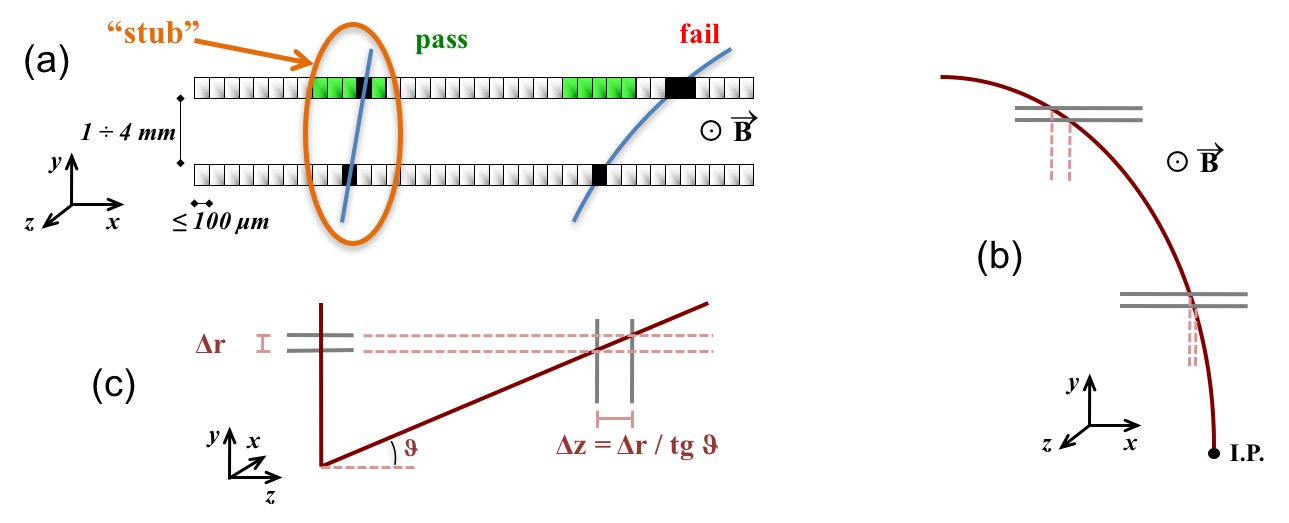
\includegraphics[width=5in]{figs/tk-upgrade/pTsketches.png}
% where an .eps filename suffix will be assumed under latex,
% and a .pdf suffix will be assumed for pdflatex; or what has been declared
% via \DeclareGraphicsExtensions.
\caption{Cluster matching in $p_\mathrm{T}$-modules~\cite{P2TrackerTDR}. (a) Correlating closely spaced clusters between two sensor layers, separated by a few mm, allows discrimination of transverse momentum based on the particle bend in the CMS magnetic field, assuming that the particle originated at the beam-line. (b) The same transverse momentum corresponds to a larger distance between signals for a given sensor spacing. (c) A larger spacing is needed in the endcap disks to achieve the same discrimination. Only tracks with \pT $> 2-3$\GeVc are transferred off-detector.
}
\label{fig:stubs}
\end{figure}

Two \pT modules are being developed for the Outer Tracker upgrade: 2S \emph{strip-strip} modules and PS \emph{pixel-strip} modules, both shown in figure~\ref{fig:2Spsmodules}.
The 2S~modules, are designed to be used at radii $r>60$\cm from the beam line, where the hit occupancies are lower and each sensor has an active area of 0.05\cm~$\times$~9.14\cm.
Both 2S~module strip layers have a pitch of 90\mum in the transverse plane, $r$-$\varphi$, and a strip length of 5.03\cm along the direction of the beam axis, $z$.
Each PS~module sensor layer has an active area of 4.69\cm~$\times$~9.60\cm, will be used at radii $20<r<60$\cm where the occupancies are highest.
The upper PS~module layers consist of an upper silicon strip sensor, and the lower a silicon pixel sensor, both with a pitch of 100\mum in $r$-$\varphi$, and a strip length in $z$ of 2.35\cm for the strips and 1.47\mm for the pixels.
The finer granularity provided by the pixel layer affords better resolution along the $z$ axis, which is crucial for vertex identification in the high \PU environment of the HL-LHC.
Further details on the two \pT modules can be found in~\cite{CMS_Upgrade_TP,P2TrackerTDR}.
 
\begin{figure}[tp]
\centering
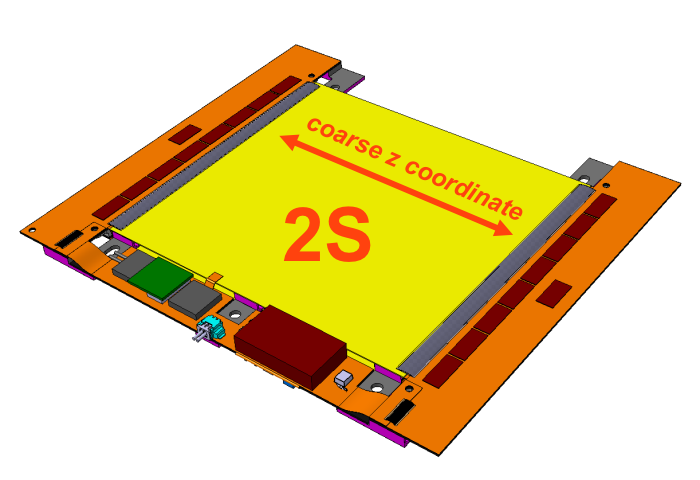
\includegraphics[width=0.55\textwidth,trim={0truecm 0truecm 0truecm 1truecm},clip]{figs/tk-upgrade/2S_assembled.png}
\hfill
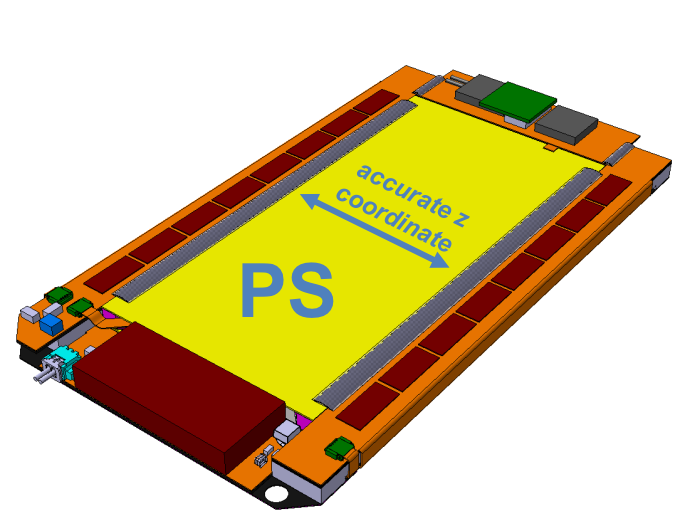
\includegraphics[width=0.44\textwidth,trim={0truecm 0truecm 0truecm 1truecm},clip]{figs/tk-upgrade/PS_assembled.png}
% where an .eps filename suffix will be assumed under latex,
% and a .pdf suffix will be assumed for pdflatex; or what has been declared
% via \DeclareGraphicsExtensions.
\caption{The 2S module (left) and PS module (right), described in the text~\cite{P2TrackerTDR}.}
\label{fig:2Spsmodules}
\end{figure}

The current proposed layout of the Phase-II Outer Tracker, referred to as the \emph{tilted barrel} geometry, is depicted in the upper diagram in figure~\ref{fig:trackerlayout}, and a previous proposal, referred to as the \emph{flat barrel} geometry, is shown in the lower diagram~\cite{CMS_Upgrade_TP}.
Both plots illustrate the PS and 2S module positions in the six barrel layers and the five endcap disks either side of the barrel, with only modules located at $|\eta| < 2.4$ being configured to send stub data off-detector.
Both geometries' names were inspired by whether or not the modules in the three innermost barrel layers being tilted so that their normals point towards the interaction region.
The advantages of the tilted geometry over the original flat barrel are that it not only improves stub-finding efficiency for tracks with large incident angles but also reduces the overall cost of the system~\cite{P2TrackerTDR}.
Due to the maturity of the preparations for the review between the three competing proposed track finding systems, discussed in Chapter~\ref{subsec:TrackFinderReview}, at the time the tilted barrel geometry was adopted for the Phase-II Outer Tracker TDR, it was decided to use the flat barrel geometry for results produced for the review.

\begin{figure}[tbp]
\centering
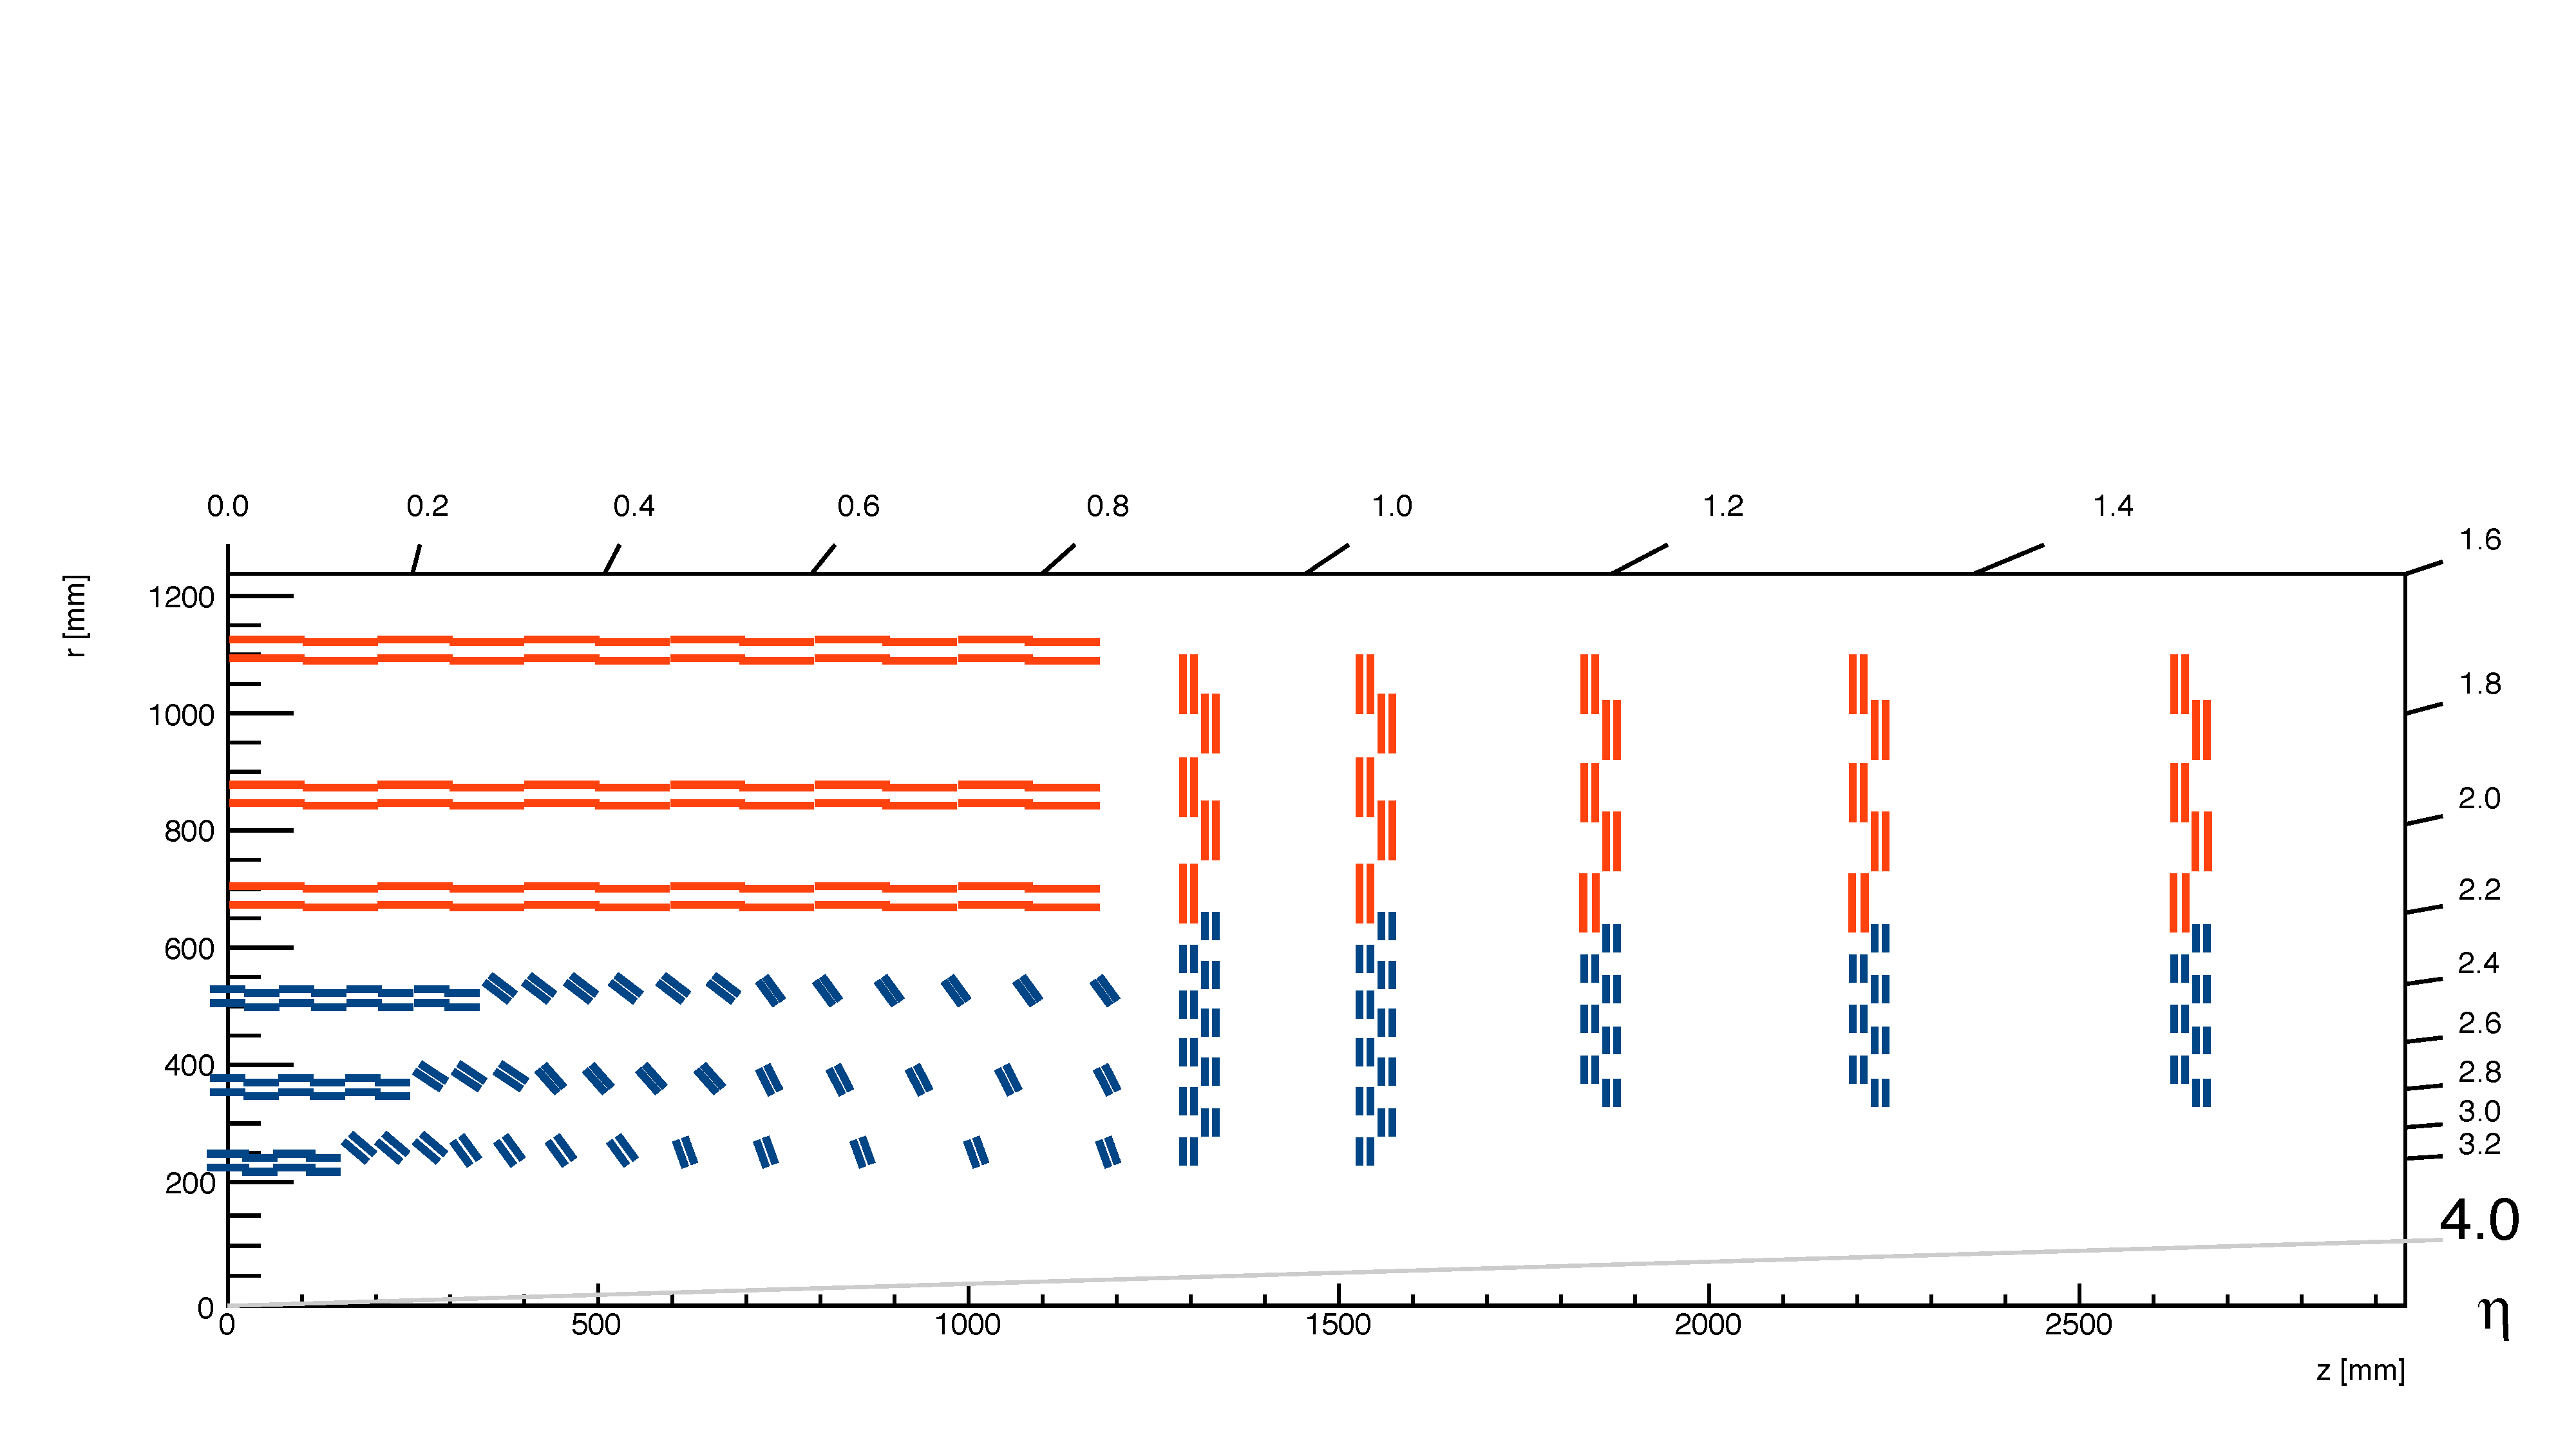
\includegraphics[width=0.8\textwidth,trim={1.1truecm 0truecm 1truecm 12truecm},clip]{figs/tk-upgrade/tiltedbarrelmap.pdf}
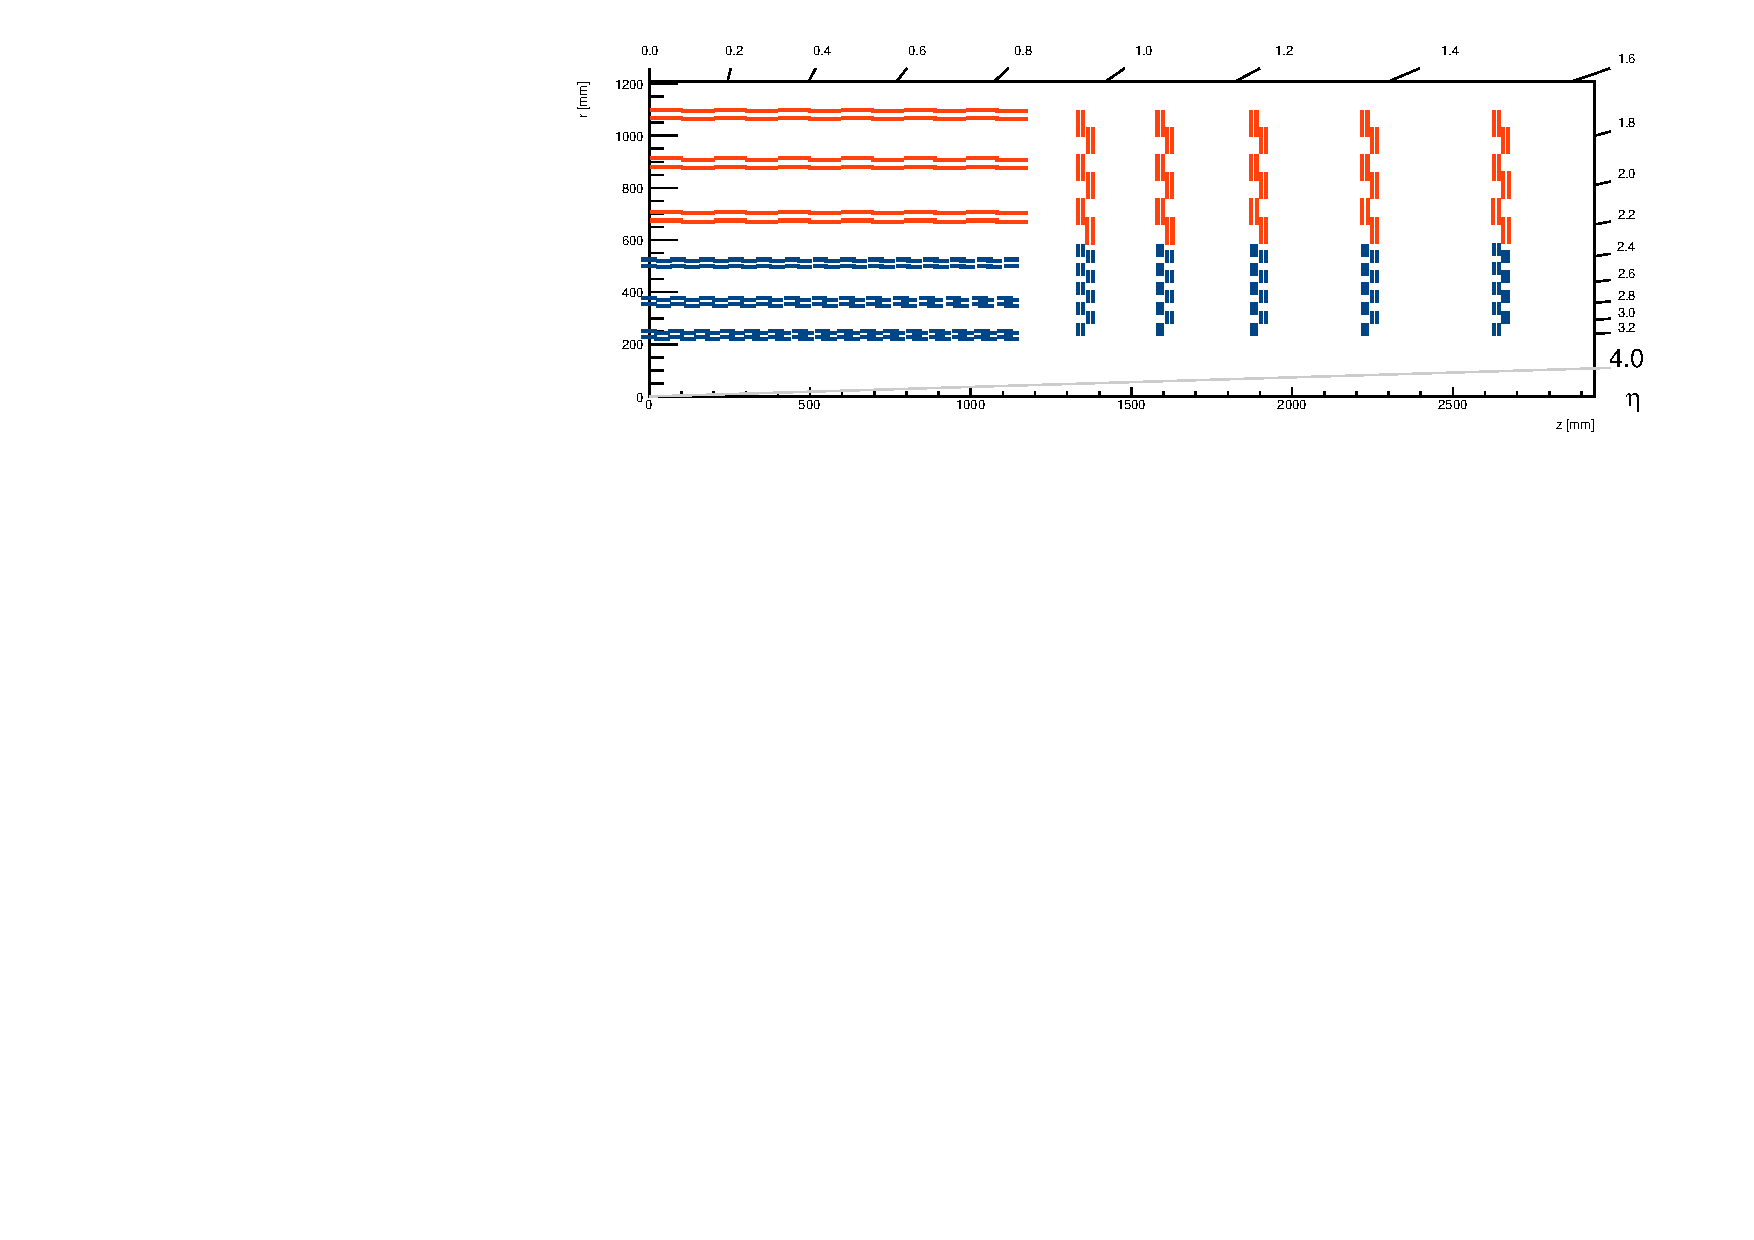
\includegraphics[width=0.8\textwidth,trim={0.7truecm 0truecm 1truecm 0truecm},clip]{figs/tk-upgrade/mersilayout.pdf}
\caption{One quadrant of the Phase-II Outer Tracker layout, showing the placement of the the PS (blue) and 2S (red) modules. The upper diagram shows the currently proposed \emph{tilted barrel} geometry~\cite{tiltedGeometry, P2TrackerTDR}, and the lower diagram shows an older proposal for the layout, known as the \emph{flat barrel} geometry \cite{CMS_Upgrade_TP}.}
\label{fig:trackerlayout}
\end{figure}

Out of the total L1 latency of 12.5\mus, $\approx 1\mus$ is required for generation, packaging and transmission of stubs from the tracker front-end electronics to the Data, Trigger and Control (DTC) system and $\approx 4\mus$ is available for the reconstruction of tracks from data arriving at the DTC, as shown in figure~\ref{fig:dataFlow}.
The rest of the available latency is allocated for the correlation of tracks with trigger primitives from the calorimeters and muon systems ($\approx 3.5\mus$), the propagation of the L1 decision to the front-end buffers ($1\mus$) and a safety margin ($3\mus$)~\cite{CMS_Upgrade_TP}.
Any Track Finder, which will take the stubs as input and output fully reconstructed tracks for the L1, proposed will be constrained by both being able to reconstruct tracks within the $4\mus$ latency constraint and how the detector is cabled to the DTC system.

\begin{figure}[tb]
\centering
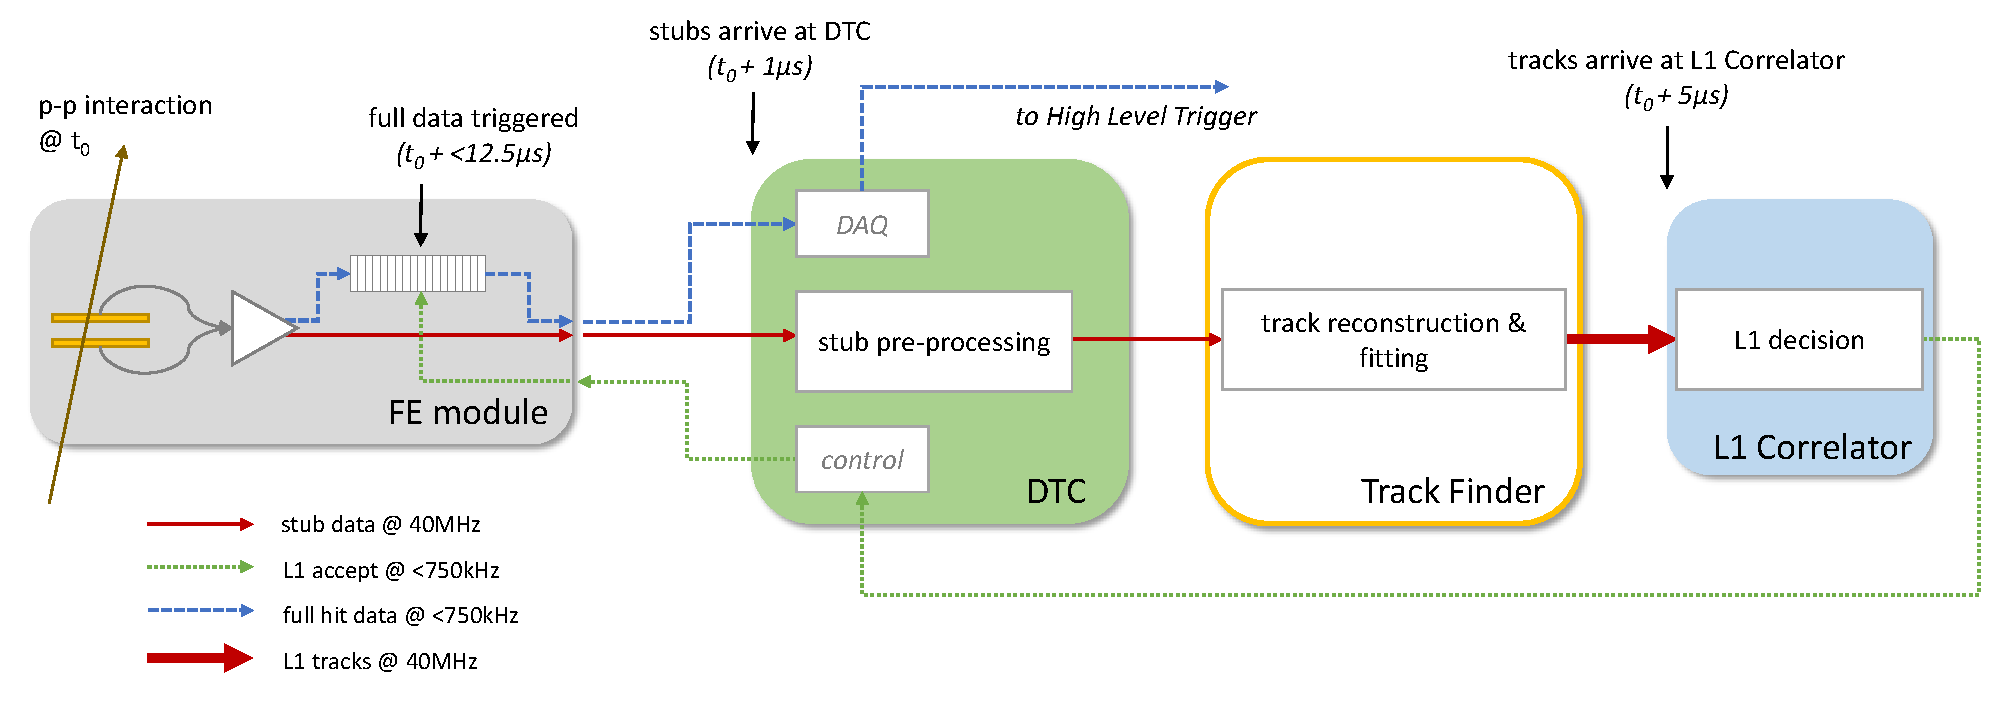
\includegraphics[width=\textwidth]{figs/tk-upgrade/dataflow.pdf}
% where an .eps filename suffix will be assumed under latex,
% and a .pdf suffix will be assumed for pdflatex; or what has been declared
% via \DeclareGraphicsExtensions.
\caption{Illustration of data-flow and latency requirements from \pt-modules through to the off-detector electronics dedicated to forming the L1 trigger decision.}
\label{fig:dataFlow}
\end{figure}

\subsection{Level-1 Track Finding Proposals}\label{subsec:TrackFinderReview}

Three different L1 track finders have been explored by the CMS Collaboration.
One uses Associative Memory (\emph{AM}) ASICs for track finding and FPGAs for track fitting, and the other two all-FPGA approaches, one using a fully Time-Multiplexed approaching using the Hough Transform (\emph{TMTT}) and the other a ``road search'' (\emph{tracklet}) algorithm to reconstruct tracks respectively.

Hardware demonstrators for each of the three proposed L1 track finder projects were constructed to prove the feasibility of each approach, which were reviewed in December 2016.
As all of the work discussed in this chapter was on the FPGA-based \HT approach, more detailed descriptions and results of both the AM and tracklet projects' approaches are not discussed here, but are given in~\cite{AM,P2TrackerTDR} and~\cite{tracklet,P2TrackerTDR} respectively.

As mentioned above, at the time of the review the flat barrel geometry was used for all the studies undertaken, as depicted in the lower diagram in figure~\ref{fig:trackerlayout}.
Unless stated otherwise, the results discussed below use the flat barrel geometry instead of the tilted barrel geometry layout.

\section{An FPGA Based Track Finding Architecture and Processor}\label{sec:TMTT}
\subsection{The Track Finding Architecture}\label{subsec:TFA}
The proposed FPGA-based Hough Transform Track Finder is a scalable, flexible and redundant design based on a fully time-multiplexed architecture, as previously demonstrated by the Phase-I Calorimeter Trigger Upgrade~\ref{paragraph:L1}, for implementation on commercially available FPGAs.
A time-multiplexed design has a number of advantages, as discussed in~\ref{paragraph:L1}, including that only a single Track Finding Processor (TFP) is required to demonstrate the full system as each processor is identical in every respect.

Unlike the Phase-I Calorimeter Trigger, it is infeasible to process the entire output of the Phase-II Outer Tracker in a single processor for a given time slice because of the limits imposed by the input and total bandwidth a single FPGA-based processor could handle.
Therefore, as it was assumed at the time of the December 2016 review that the DTC system would be arranged such that it forms octants~\footnote{These detector octants are not uniform as the geometry of the tracker does not have an exact eight-fold symmetry} (\ie 45 degree $\varphi$-sectors, referred to as \emph {detector octants}) in the tracker, the baseline system proposed was divided into \emph{processor octants} that were offset from the detector octants by $\approx 22.5$ degrees in $\phi$, in order to handle data duplication across hardware boundaries.
This baseline system is illustrated in figure~\ref{fig:tmttarch}.

\begin{figure}[t]
\centering
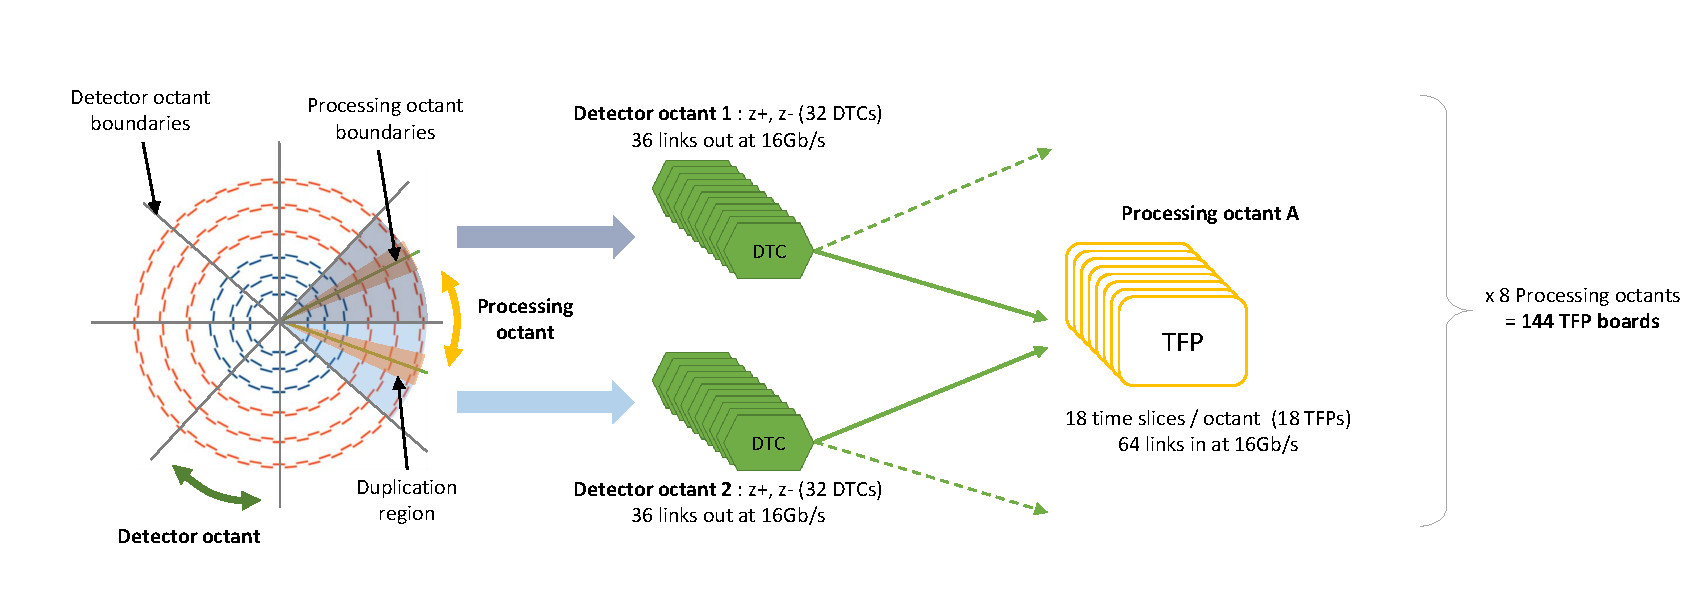
\includegraphics[width=1.00\textwidth]{figs/tk-upgrade/tmttarch.pdf}
\caption{The baseline system architecture uses two neighbouring DTCs to time-multiplex and duplicate stub data across processing octant boundaries, before each DTC transmits 50\% of its data to one TFP and 50\% to the neighbouring TFP Based off current electronics and high speed links available, the data requires 18 TFPs per processing octant (one for each time slice, resulting in a full system requiring 144 TFPs).}
\label{fig:tmttarch}
\end{figure}

A hardware demonstrator of the baseline system consisting of five Imperial Master Processor Virtex-7 (MP7) cards~\cite{mp7ref}, capable of processing one phi-octant of the tracker with a time-multiplexing factor of 36, was used to validate the feasibility of the proposed full system using currently available hardware for the December 2016 review.
All of the results achieved, and a complete description of the system, are given in~\cite{TMTT_JINST}.

\subsection{The Track Finding Processor}\label{subsec:TFP}
The Track Finding Processor (figure~\ref{fig:TFP}) consists of four self-contained components:
\begin{itemize}
\item {\bf Geometric Processor (GP)} - responsible for pre-processing the stubs from the DTC.
\item {\bf Hough Transform (HT)} - a highly panellised initial coarse track finding.
\item {\bf Kalman Filter (KF)} - cleans tracks, precisely fits helix parameters and removes fake tracks.
\item {\bf Duplicate Removal (DR)} - a final pass filter that uses the precise fit information to remove duplicate tracks generated by the \HT.
\end{itemize}

\begin{figure}[!h]
\centering
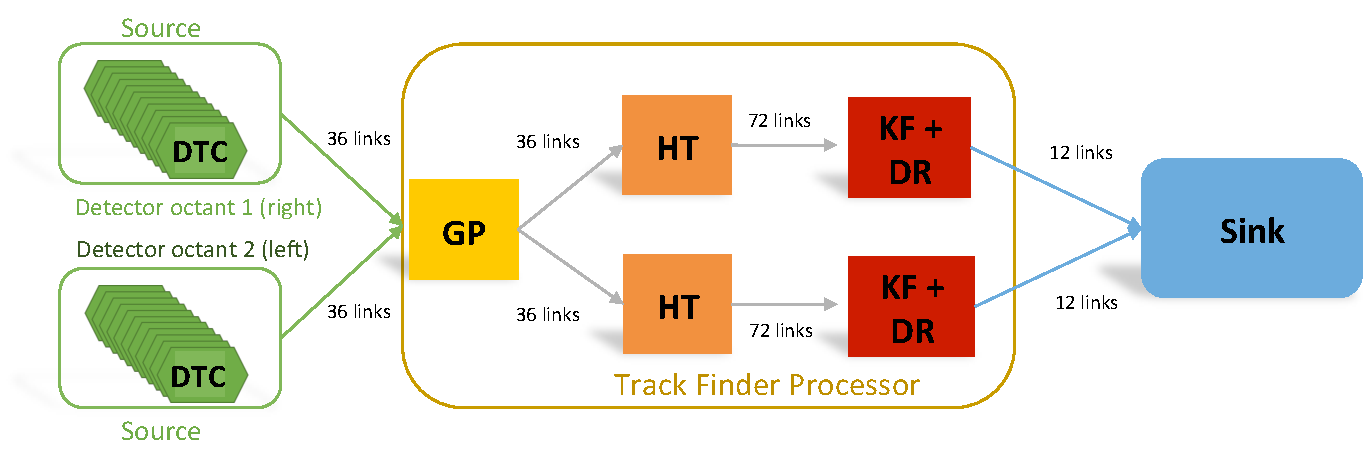
\includegraphics[width=0.78\textwidth]{figs/tk-upgrade/demoslice1.pdf}
% where an .eps filename suffix will be assumed under latex,
% and a .pdf suffix will be assumed for pdflatex; or what has been declared
% via \DeclareGraphicsExtensions.
\caption{The four self-contained logical components of the Track Finding Processor, where each block represents a single FPGA. The two FPGAs for the two detector octant sources and the sink FPGA and the optical links between all components are also shown.}
\label{fig:TFP}
\end{figure}

\subsubsection{Geometric Processor}\label{subsubsec:GP}
Each GP performs two tasks, firstly the conversion of the 48-bit DTC stubs into a 64-bit format extended format that is used to reduce the HT processing load and secondly the assignment of stubs to thirty six sub-sectors, two sub-sectors in $\phi$ and eighteen in $\eta$ (where $\eta$ is the pseudo-rapidity). 
This division of the processing octants simplifies the task of the downstream logic required, allowing the track finding to be carried out independently and in parallel within each sub-sector. 
The relatively fine $\eta$ binning ensures that any track found by the \rphi HT is consistent in the \rz plane. Stubs compatible with more than one sub-sector, usually due to track curvature in $\phi$ are duplicated. 
The routing of stubs to sub-sectors occurs in three stages: a rough $\eta$ sorting into six bins, a fine $\eta$ sorting into three bins and a $\phi$ sorting into two bins. 
Each block in this router is highly reconfigurable and can easily be adapted to any alternative sub-sector definition.

\subsubsection{Hough Transform}
The Hough Transform algorithm is a widely used means of detecting geometric features in digital image processing \cite{HT} and is used by the TFP to find charged particles with \pT > 3\GeV in the \rphi plane. 

Within the tracking volume, permeated by a homogeneous 3.8T magnetic field ($B$), a radius of curvature ($R$) can be described as a function of its\pT and charge $q$:

\begin{equation}
R = \frac{\pt}{0.003\,qB} \;
\label{eq:R}
\end{equation}

Assuming, to first order, that $R$ is constant, by neglecting energy losses such as through multiple scattering, and that only primary tracks from or near the primary interaction point are considered (other such tracks are not typically relevant to the L1 trigger), a stub with coordinates ($r$,$\varphi$) is related to $R$ by:

\begin{equation}
\frac r{2\,R} = \sin\left(\varphi-\phi\right) \;
\label{eq:stub_R}
\end{equation}

where $\phi$ is the angle of the track in the transverse plane at the origin \cite{markthesis}. 
For large \pT (> 3\GeV) and thus large $R$, the small angle approximation can be used. Combining Eq.~\ref{eq:R} and Eq.~\ref{eq:stub_R}, one produces the key formula showing the transformation from stub positions to straight lines in the track parameter plane (Hough-space):

\begin{equation}
\phi = \varphi - \frac{0.0015\,qB}{\pt}\cdot r \;
\label{eq:localHT}
\end{equation}

The point of intersection of these lines in Hough-space would therefore correspond to a circle in the \rphi plane which is consistent with the primary interaction point and all stubs involved.
As the line gradients in Hough-space is given by the radius of the stubs, they will always be positive, the stub radius is transformed to $r_{58} = r - 58cm$ in order to utilise a larger phase space, which leads to fewer \textit{fake} (in that the found track does not match to a simulated particle) and duplicated tracks.

Given that $R$ for the lowest \pT track (3\GeV) to be considered is greater than the outer radius of the tracking detector ($r$ = 1.2m), all relevant particles are expected to traverse through at least six barrel layers or endcap disks. 
The threshold for the identification of a track candidate however, is set at a minimum of five detector layers or disks in order to allow for detector or readout inefficiencies. 
This threshold can be further reduced to four layers to account for the reduced geometric coverage between $0.89 < \eta < 1.16$ or for dead detector layers or disks.

A more detailed description of the firmware implementation of the \HT for the demonstrator system is discussed in~\cite{IEEE} and~\cite{TMTT_JINST}.

\subsubsection{Kalman Filter}\label{subsubsec:KF}
\editComment{More detail - including on the covariance matrix ...}
Coarse \rphi helix parameters out of the \HT are used as the initial variables for track finding, with the segment assignment also providing a good seed value.
Given that in simulation over half the track candidates from by the HT are considered to be \textit{fake} or contain at least one stub associated with another particle, a Kalman Filter is used to both remove these incorrect stubs and reject fake tracks. 

In addition to the advantages of the Kalman filter for track reconstruction discussed by Fr{\"u}hwirth in \cite{Fruhwirth:1987fm}, the algorithm has several aspects making it suitable for FPGA implementation compared to global track fitting methods, namely the matrices:

\begin{itemize}
\item {are small.}
\item {are size independent of the number of measurements.}
\item {only involve the inversion of a small matrix.}
\end{itemize}

The initial estimates, or \textit{state}, of the track parameters and their uncertainties, $\chi^2$ value and other status information are updated by the KF iteratively applying stubs to update the state following the Kalman formalism, decreasing the uncertainty in the state. 
Each update of the state can be filtered on number of configurable criteria, including \pT, $\chi^2$, and the minimum number of stubs from PS modules, and can take into account and skip missing missing layers due to missing or incorrect stubs.
In the event multiple stubs are found on the same layer, each can be propagated with up to the four best states being kept and presented to a final state selector, with preference given to states with the fewest missing layers and the smallest $\chi^2$.
The final fit is always performed after a fixed period of time, so consequently there is no truncation in the traditional sense as all candidates will be read out, although events such as dense jets with many candidates and stubs per candidate will only be partially filtered.

A greater in-depth discussion of the mathematics and implementation of online track reconstruction using Kalman Filters on FPGAs in \cite{SSummers}.

\subsubsection{Duplicate Removal}
At the input to the DR, over half of the track candidates are unwanted duplicate tracks created by the HT.
By understanding how the HT produces these duplicate tracks, a more elegant and subtle DR algorithm can be used instead of having to compare pairs of tracks to see if they are the same as each other.
This approach is illustrated in figure~\ref{fig:DR}, where five stubs (blue lines in Hough Space) produce three candidates (green and yellow cells).
As all three candidates contain the same stubs, they will be fitted with identical helix parameters in the same cell (the yellow cell) regardless of the original HT cell.
The algorithm accepts only tracks whose fitted parameters are consistent to those that the HT found them in initially. There is however, a small subtlety, given that the algorithm eliminates unique tracks whose fitted parameters were not consistent, which results in the loss of a few percent of efficiency. 
By performing a second pass through the rejected tracks and rescuing those which are unique the lost efficiency can be recovered.

\begin{figure}[!h]
\centering
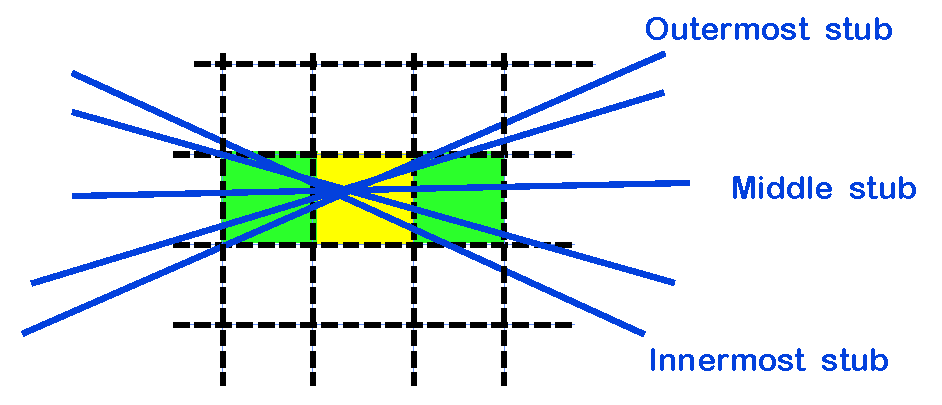
\includegraphics[width=0.80\textwidth]{figs/tk-upgrade/A50_algo.pdf}
% where an .eps filename suffix will be assumed under latex,
% and a .pdf suffix will be assumed for pdflatex; or what has been declared
% via \DeclareGraphicsExtensions.
\caption{Illustration of how duplicates are formed by the \rphi \HT.}
\label{fig:DR}
\end{figure}

A more detailed description of the firmware implementation of the \DR for the demonstrator system is discussed in~\cite{TMTT_JINST}.

\section{Simulation Studies}\label{sec:TmttSimStudies}
\editComment{Add legend to plots and reduce size of points on plots by half}
\editComment{Make tables fit on page!}
\editComment{Update axis labels (units too) and use same resolution definitions as the JINST paper + TDR}

During the development of the \emph{TMTT} demonstrator system both before and following the December 2016 review, the author was involved in a number of simulation studies, the more substantive of which are presented below.
All of the results discussed use a common set of definitions, as defined in Chapter~\ref{subsubsec:helixParameter}, and the track fitters discussed use digitised output from the \HT.

\subsubsection{Common definitions}\label{subsubsec:helixParameter}
A number of parameters and metrics are used to describe tracks and how well the track fitters have reconstructed them are used throughout this chapter and are given below.

\paragraph{Helix Parameters}

Five helix parameters are used to parametrise the helical path of a charged particle as it travels through the detector.
They are:

\begin{itemize}
\item $\mathbf{\frac{1}{R}}$ - the inverse radius of curvature of the track. As the magnetic field in the tracker is constant and the radius of curvature is proportional to the transverse momentum of the track, results are quoted in terms of $\frac{q}{\pT}$ (where q is the charge of the particle).
\item $\mathbf{\phi_{0}}$ - the track direction at the point of closest approach to the interaction point.
\item $\mathbf{z_{0}}$ - the z position of the helix at the point of closest approach to the interaction point.
\item $\mathbf{\tan(\lambda)}$ - the tangent of the \emph{dip} angle, related to $\eta$ by $\tan(\lambda) = \sinh (\eta)$ and expressed in terms of $\eta$ for the results presented.
\item $\mathbf{d_{0}}$ - the \emph{impact parameter}, \ie the distance of the track vertex from the interaction point in the $x-y$ plane. The \HT and track fitting algorithms discussed all assume that all tracks originate at the interaction point, \ie $d_{0} = 0$. As such, results involving this helix parameter are not given below.
\end{itemize}

\paragraph{Reconstructed Track Definition}
The common definitions of track reconstruction efficiency~\cite{TMTT_JINST} used for the three proposed L1 Track Finder systems are used for the results presented in this chapter:

\begin{itemize}
\item The reconstruction efficiency is measured relative to all generated charged particles from the primary interaction that produce stubs in at least four layers of the tracker and lies within $\pT > 3\GeV$, $|\eta| < 2.4$, $|z_{0}| < 30\cm$ and $d_{xy} < 1\cm$.
\item A track is a defined as being correctly reconstructed or \emph{matched} if the reconstructed track has stubs associated to the particle in at least four tracker layers.
\item Tracks which fail this matching criteria are known either as \emph{unmatched} or \emph{fake} tracks.
\item If all a reconstructed track's stubs originated from the same particle, the track is defined as being \emph{perfectly} reconstructed. 
This stricter latter definition is only used in quoting results from the entire chain (\ie all four components of the TFP discussed in Chapter~\ref{subsec:TFP}), as the presence of stubs incorrectly associated to a track is to be expected if only part of the TFP chain has been run.
\item If the reconstruction of a charged particle produces more than one track, these additional tracks are considered to be \emph{duplicates}.
\end{itemize}

\subsection{Linearised $\chi^{2}$ Track Fitter}\label{subsec:chi2}
Whilst the Kalman Filter was used as a track fitter for the December 2016 hardware demonstrator, a Linear Regression (LR)~\footnote{The LR fitter~\cite{TMTT_FLP} was developed as an alternative to the KF and exploits the fact that sufficiently high \pT tracks should form a straight line in the \emph{\rphi} and \emph{r-z} planes to perform independent fits in each planes.} and a Linearised $\chi^{2}$ fitting algorithms were also explored.

The studies into a linearised $\chi^{2}$ track fit were initially motivated by the \emph{TMTT} project anticipating potential time and resource pressures in developing all the components of a complete track finding system that could be implemented in hardware due to the project being formed significantly after the other two L1 track finder projects.
Following discussions with both the \emph{tracklet} and \emph{AM} projects, it was decided that the use of a linearised $\chi^{2}$ fit based off the one proposed by the \emph{tracklet} project would be investigated.
The general form of the $\chi^{2}$ fit and the derivation of the track derivatives required by the algorithm were provided in a private communication~\cite{CMS_DN-14-043} and were used to produce our own implementation of the track fitting algorithm.

A linearised $\chi^{2}$ fit makes use of residuals between the stubs and the seeded track that minimise $\chi^{2}$ of the fit in order to calculate improved helix parameters for the track candidate.
The general form of the $\chi^{2}$ fit describing how these hit residuals are used to obtain a fit of a track's helix parameters is detailed in Chapter~\ref{subsubsec:chi2maths}.
A discussion of the development and outcomes of the software implementation of the fitting algorithm are given in Chapters~\ref{subsubsec:chi2software,subsubsec:chi2outlook}.
The calculation of the track derivatives for the barrel layer and endcap disk hits used by the algorithm, including a correction factor for $\phi$ in the outer disks to account for the fact that these modules do not point directly towards the interaction point, are given in full in Appendix~\ref{app:chi2}.

All the results presented involve the use of a \emph{Seed Filter} (SF) stage which was run following the \HT stage for both the Linear Regression and Linearised $\chi^{2}$ fitting algorithms.
This process remove stubs in a \HT cell which are inconsistent with a straight line in the \emph{r-z} plane and filters out both fake tracks and stubs incorrectly assigned to tracks (also referred to as \emph{fake} stubs).

\subsubsection{General Form of a $\chi^{2}$ Fit}\label{subsubsec:chi2maths}
For the general form of a $\chi^{2}$ fit for a track, $f$, described by its helix parameters, $\overrightarrow{h}$, and 
the position of its $i$ hits (\ie stubs) given at $s_{i}$, we initially linearly expand the projection of the track, $f_{i}$, around the estimate of the helix parameters $\overline{h}$:

\begin{equation}
f_{i}(\overrightarrow{h} ) = f_{i}(\overrightarrow{h} + \delta \overrightarrow{h}) \;
                           = f_{i}(\overline{h} + \delta \overrightarrow{h} \frac{\partial f_{i}}{\partial \overrightarrow{h}} + \mathcal{O}(\delta \overrightarrow{h}^{2}) \;
\label{eq:chi1}
\end{equation}

The $\chi^{2}$ of such a track is expressed as:

\begin{equation}
\begin{split}
\chi^{2} &= \sum_{ij} \big(f_{i}(\overrightarrow{h}) - s_{i} \big) V^{-1}_{ij}  \big(f_{j}(\overrightarrow{h}) - s_{j} \big)  \\
         &= \sum_{ij} \big( f_{i}(\overline{h})  - s_{i} + \delta \overrightarrow{h} \frac{\partial f_{i}}{\partial \overrightarrow{h}} \big) V^{-1}_{ij}  \big( f_{j}(\overline{h})  - s_{j} + \delta \overrightarrow{h} \frac{\partial f_{j}}{\partial \overrightarrow{h}} \big)  \\
         &= \sum_{ij} \big( \delta f_{i} + \delta \overrightarrow{h} \frac{\partial f_{i}}{\partial \overrightarrow{h}} \big) V^{-1}_{ij}  \big( \delta f_{j} + \delta \overrightarrow{h} \frac{\partial f_{j}}{\partial \overrightarrow{h}} \big)
\end{split}
\label{eq:chi2}
\end{equation}

where $\delta f_{i} \equiv f_{i}(\overline{h}) - s_{i}$ are the residuals between the expected position of the track (given by the seed helix parameters) and the position of the track given by the stub, and $V^{-1}_{ij} = diag(\sigma^{2}_{ii})$ is the variance matrix which describes the uncertainty associated to the measurement of the stubs.

By is minimising $\chi^{2}$, $\delta h$ can be determined:

\begin{equation}
0 = \frac{\partial \chi^{2}}{\partial \delta \overrightarrow{h_{k}}} = \sum_{ij} \frac{\partial f_{i}}{\partial \delta \overrightarrow{h_{k}}} V^{-1}_{ij} ( \delta f_{j} + \delta \overrightarrow{h} \frac{\partial f_{j}}{\partial \overrightarrow{h}} ) + \sum_{ij}	( \delta f_{i} + \delta \overrightarrow{h} \frac{\partial f_{i}}{\partial \overrightarrow{h}} ) V^{-1}_{ij} \frac{\partial f_{j}}{\partial \delta \overrightarrow{h_{k}}}  \;
\label{eq:chi3}
\end{equation}

By defining the matrices $D_{ij} = \frac{\partial f_{i}}{\partial h_{k}}$ and $M = D^{T} V^{-1} D$, equation~\ref{eq:chi3} can be rewritten and solved for $\delta h$:

\begin{equation}
0 = D^{T} V^{-1} \delta f + M \delta h \Rightarrow \delta h = - M^{-1} D^{T} \delta f \;
\label{eq:chi4}
\end{equation}

Therefore equation~\ref{eq:chi4} provides a simple linear form for how the track helix parameters should be updated for a set of residuals with respect to the seed track candidate.

Similarly the $\chi^{2}$ of the fit can also be expressed in a linear form:

\begin{equation}
\begin{split}
\chi^{2} &= (\delta f + D \delta h)^{T}(\delta f + D \delta h) \\
         &= (\delta f - DM^{-1}D^{T}\delta f)^{T} (\delta f - DM^{-1}D^{T}\delta f) \\
         &= \delta f^{T} (1- DM^{-1}D^{T}) (1- DM^{-1}D^{T}) \delta f \\
         &= \delta f^{T} (1- DM^{-1}D^{T}) \delta f \\
         &= \delta f^{T} \delta f - \delta f^{T} DM^{-1}D^{T} \delta f \\
         &= \chi^{2}_{seed} + \delta f^{T} D \delta \overrightarrow{h} 
\end{split}
\label{eq:chi5}
\end{equation}

As the linear forms of equations~\ref{eq:chi4} and~\ref{eq:chi5} consist of repeated addition and multiplication operations of the matrices involved, they are naturally suitable for implementation on an FPGA.

For whilst FPGAs can easily perform such operations, potential complications arise when considering the calculation of the track derivatives that form the elements of $D$ which would not trivial given the presence of a large number divisions and trigonometric functions for the endcaps' derivatives.
Therefore, any implementation in firmware for an FPGA will require the use of lookup tables containing the precomputed values of the derivatives in order to quickly update a track's helix parameters without exceeding latency budgets.

\subsubsection{Software Results}\label{subsubsec:chi2software}
\editComment{Results in this subsub section have been made with 100 ttbar+pu200 events. 
This is due to several bugs being discovered in the final version of the TMTT code for the flat geometry used to produce these results, which was not present during the development of this algo.
As the bug had a LARGE impact on the results, a low stats run has been done in order to not to delay the completion of this chapter draft any longer than it already has been!
The larger stats (~1000 to 5000 events) runs are currently in progress.}

From equations~\ref{eq:chi4} and~\ref{eq:chi5} and the track derivatives derived in Appendix~\ref{app:chi2}, a software implementation of the linearised $\chi^{2}$ track fit algorithm was developed.
Initially this implementation used exact floating point mathematics in order to validate the algorithm, before a version using approximated expressions of the track derivatives was developed.
The motivation behind this was to reduce the number of variables that the matrix of derivatives would depend on in order to simplify (and reduce resources required for) any future tabulation of the matrix.

\begin{table}[htbp]
\topcaption {Track finding performance on simulated \ttbar events at a \PU of 200, after the \HT and the full chain for  both the exact floating point and approximated calculations of the track derivatives used by the $\chi^{2}$ track fit.
The track finding efficiencies following each stage are given using the efficiency definitions given in Chapter~\ref{subsubsec:helixParameter}, along with the mean number of tracks and the fraction of those tracks which are either fake or duplicate tracks.
\editComment{Ermm ... get table to fit onto page!}
}

\label{tab:chi2-exactVsApprox}
  \centering
\resizebox{\textwidth}{!}{
% This increases column spacing.
  \addtolength{\tabcolsep}{1ex}
% This right-aligns numbers in column, but centers them under column title.
  \begin{tabular}{ccr@{\hspace{4ex}}r@{\hspace{4ex}}r@{\hspace{4ex}}r@{\hspace{4ex}}r@{\hspace{4ex}}r@{\hspace{4ex}}}
   \hline
   \bf{Stage} & \bf{Efficiency [\%]} & \bf{``Perfect'' Efficiency [\%]} & \multicolumn{1}{r}{\bf{Mean \# of tracks}} & \multicolumn{1}{r}{\bf{\% of fakes}} & \multicolumn{1}{r}{\bf{\% of duplicates}}  \\
        \hline
   HT &  97.0 & 43.1 & 351.2 & 43.9 & 37.0 \\  
   \hline
   $\chi^{2}$+DR & 95.0 & 85.8 & 86.4 & 15.7 & 9.5 \\
   (floating point) & & & & & \\
   \hline
   $\chi^{2}$+DR & 94.9 & 85.6 & 87.4 & 15.5 & 10.9 \\  
   (approximated) & & & & & \\   
%   \hline
%   KF+DR & 94.1 & 94.1 & 82.1 & 21.1 & 4.5 \\
   \hline
   
 \end{tabular}}
 \addtolength{\tabcolsep}{-1ex}
\end{table}

Table~\ref{tab:chi2-exactVsApprox} shows how the tracking performance compares between the floating point maths and ``approximated'' maths versions of the algorithm compare against each other and from the raw track finding output from the \HT.
It can be seen that whilst the \HT finds tracks with high efficiency, over half have at least one incorrectly associated stub and a significant number of the tracks found are fake or duplicated tracks.
Both floating point and approximated maths implementations give comparable results, indicating that the approximations made are acceptable.
The $chi^{2}$ track fit increases the purity of the reconstructed tracks by a factor of two and eliminating the majority of the fake tracks, whilst the \DR algorithm removes the majority of the duplicates.

Figure~\ref{fig:chi2HelixParametersResVsEtaApproxVsExact} shows that resolutions of the four track parameters as a function of $\eta$ from primary tracks in \ttbar events at \PU of 200 for both maths implementations of the algorithm.
The resolutions compare well not just between the two implementation of the algorithm's mathematics, but also with those obtained with offline track reconstruction~\cite{P2TrackerTDR}.
As offline reconstruction is able to use more sophisticated reconstruction techniques using all information from the detector, this guarantees that the tracks found will be useful to the L1 trigger.


\begin{figure}[htb]
\centering
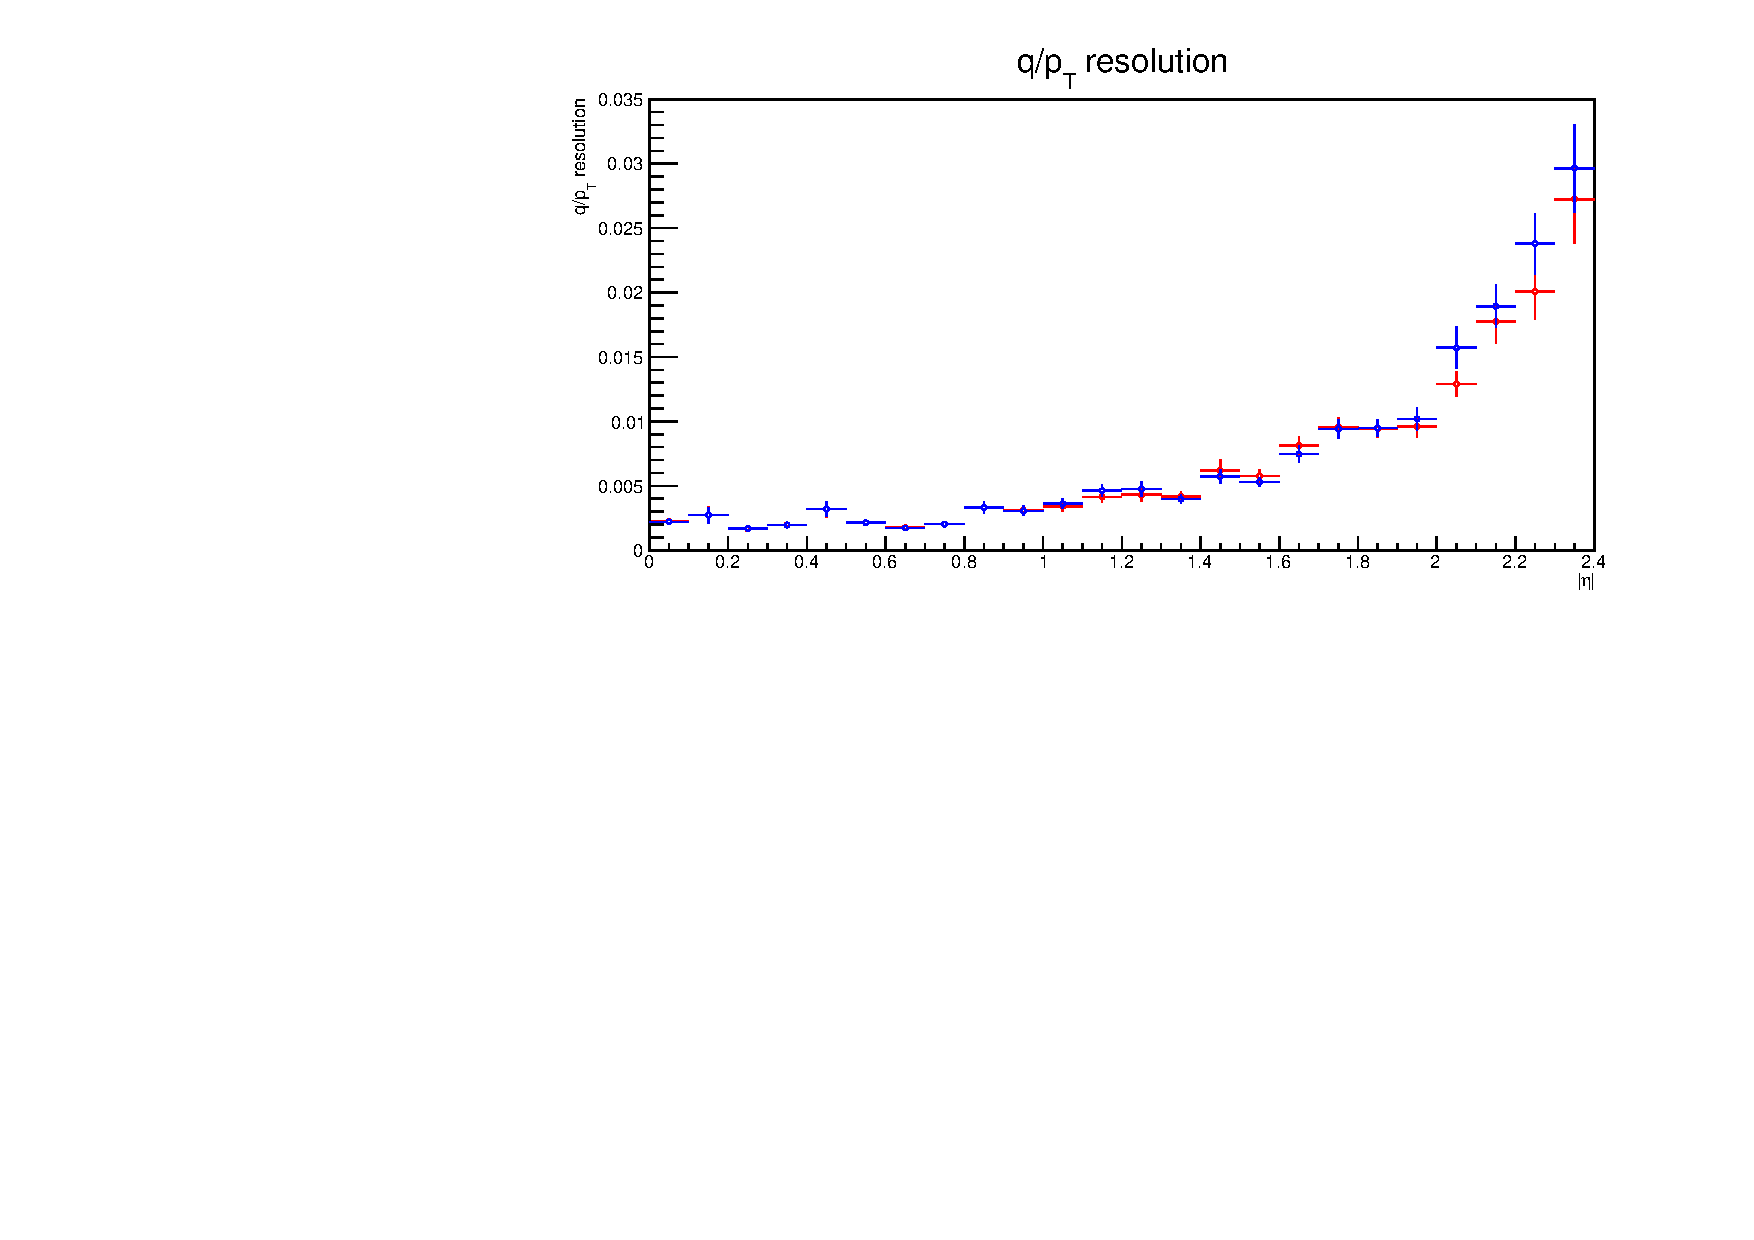
\includegraphics[width=0.47\textwidth]{figs/tk-upgrade/results-chi2fitter/qOverPtResVsEta_It_1_ApproxVsExact.pdf}
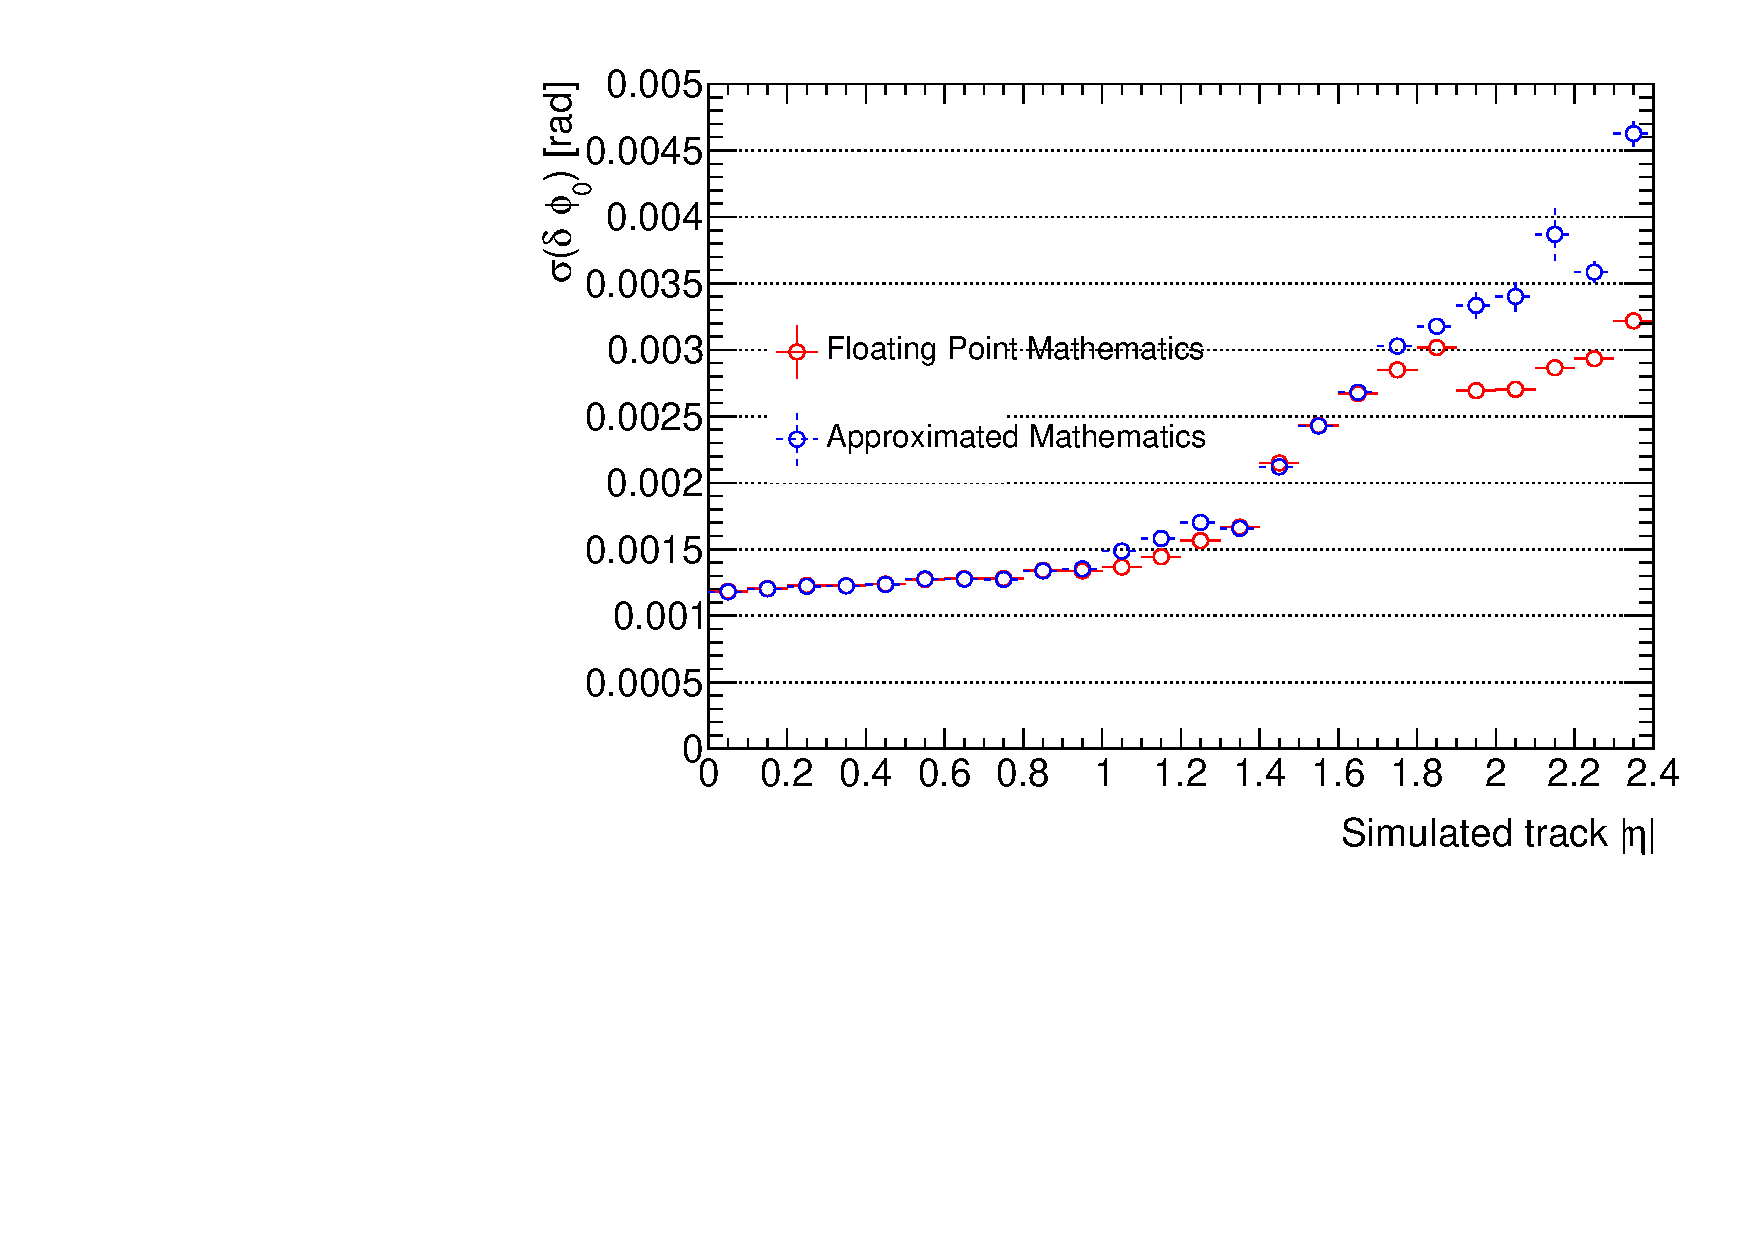
\includegraphics[width=0.47\textwidth]{figs/tk-upgrade/results-chi2fitter/phi0ResVsEta_It_1_ApproxVsExact.pdf}
\\
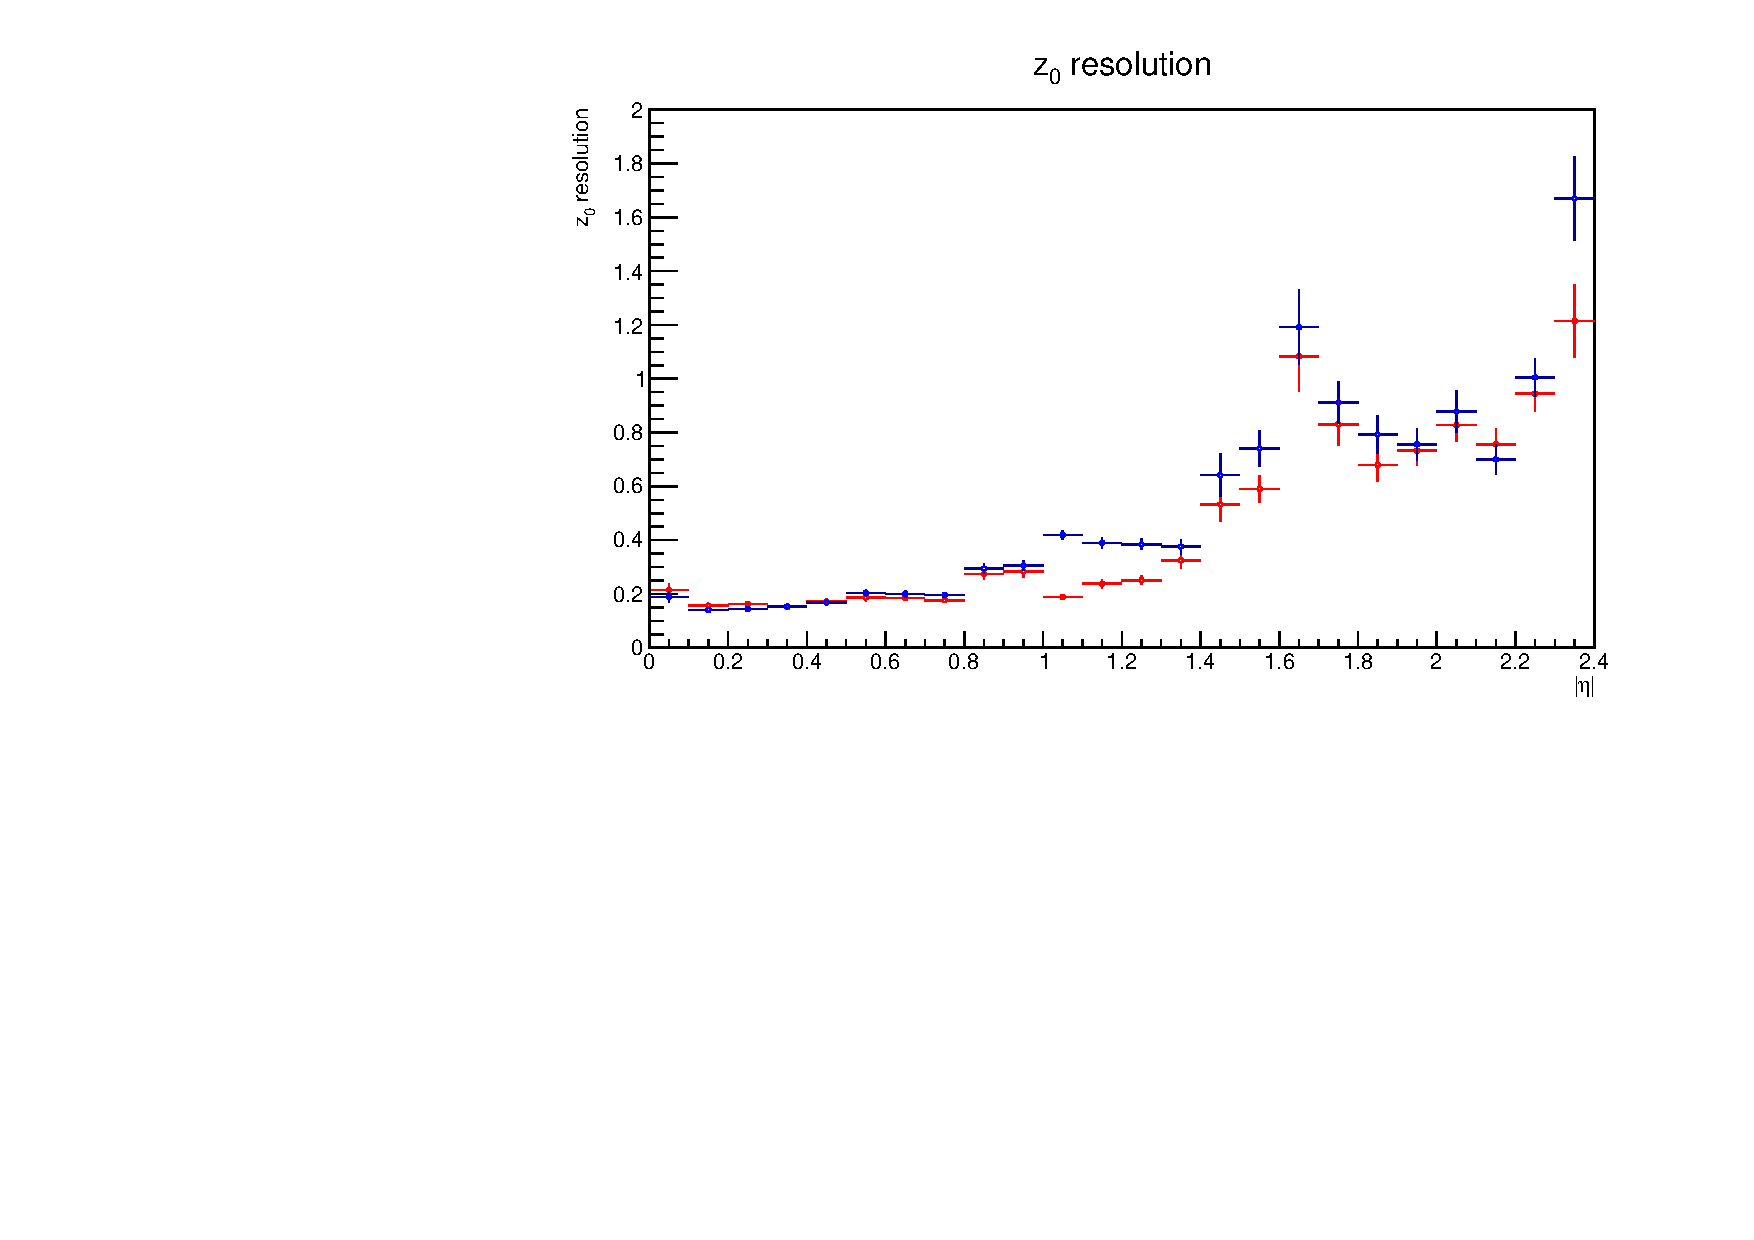
\includegraphics[width=0.47\textwidth]{figs/tk-upgrade/results-chi2fitter/z0ResVsEta_It_1_ApproxVsExact.pdf}
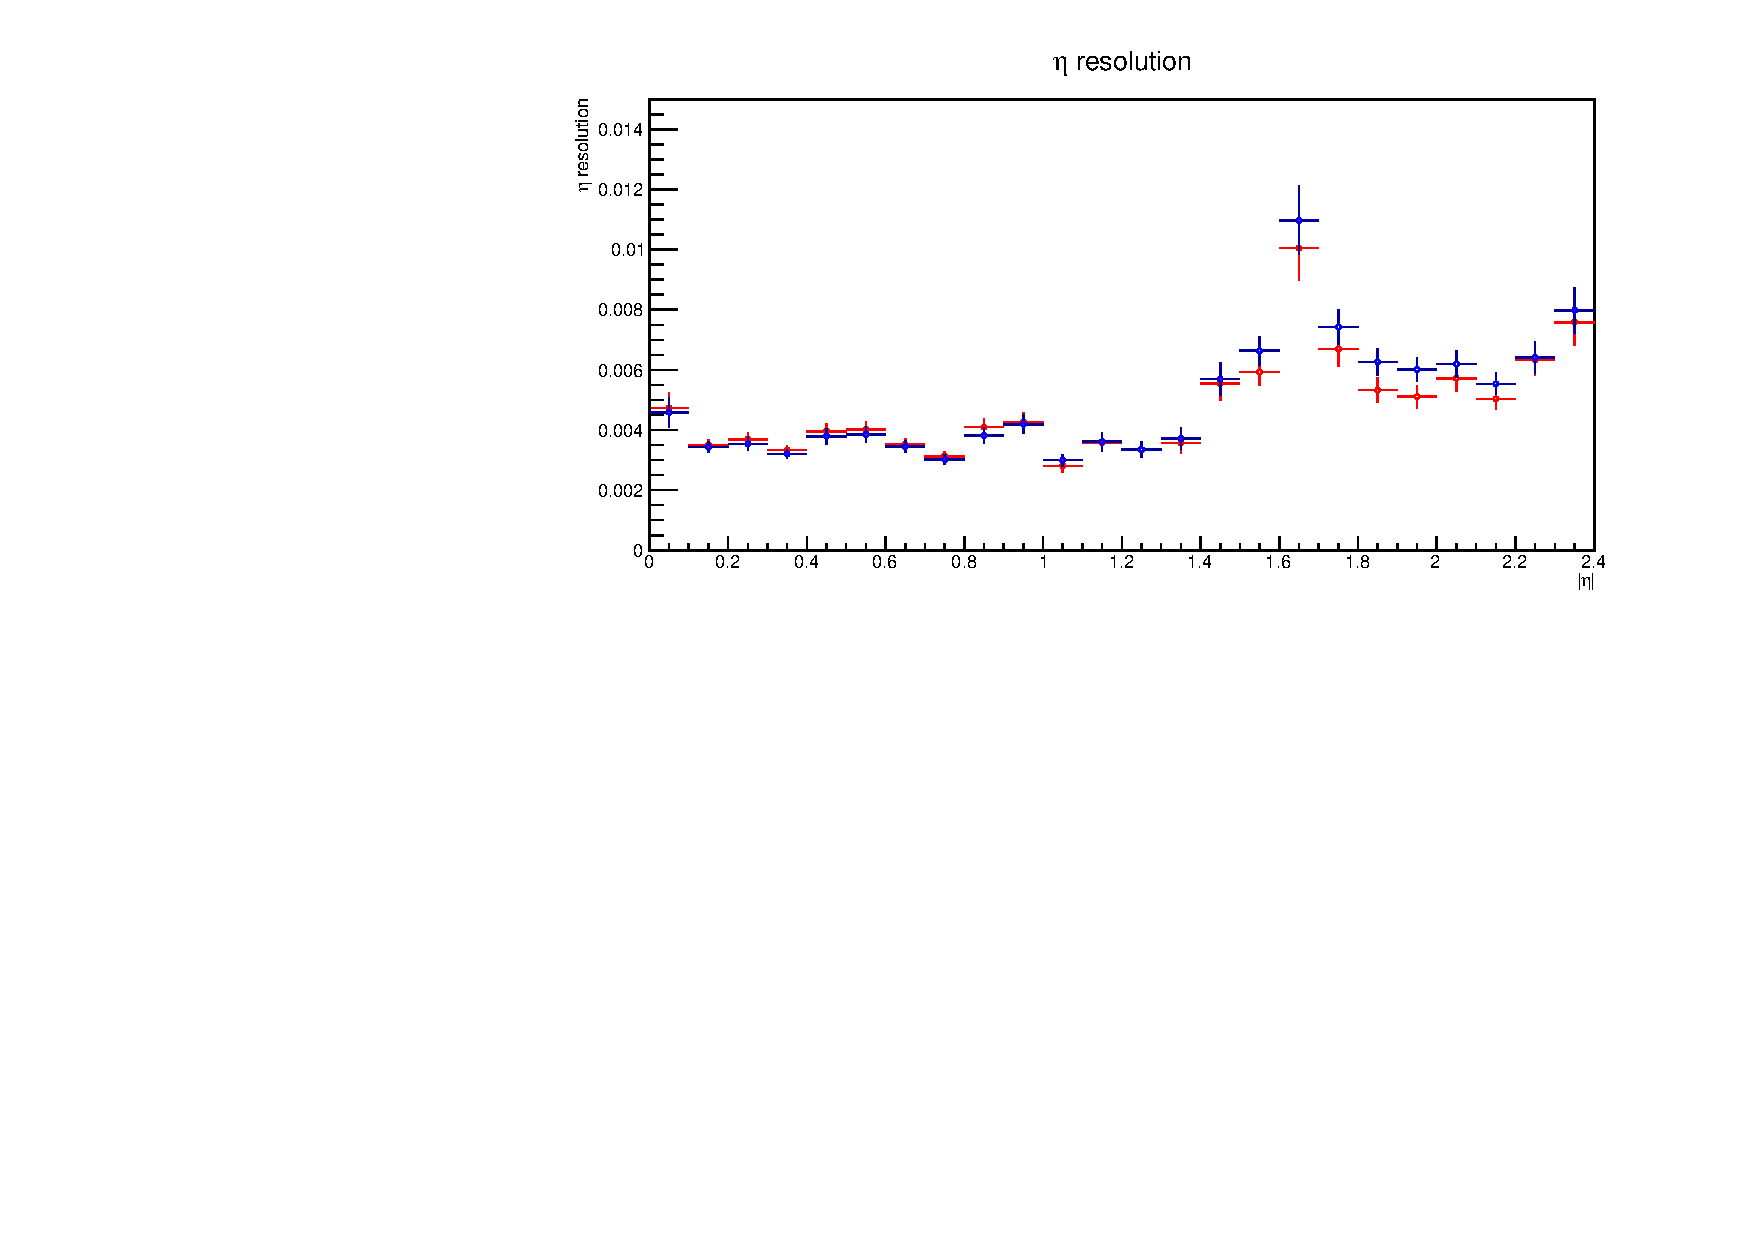
\includegraphics[width=0.47\textwidth]{figs/tk-upgrade/results-chi2fitter/etaResVsEta_It_1_ApproxVsExact.pdf}
\caption{
\pt resolution, $\phi$ resolution, $z_{0}$ resolution and $\eta$ resolution measured for primary reconstructed tracks in simulated \ttbar events at \PU of 200 for the floating point (red) and approximated maths (blue) implementations of the linearised $\chi^{2}$ fit algorithm for a single fitting iteration.
\editComment{Make plots bigger!}
\editComment{Increase stats from 100!}
}
\label{fig:chi2HelixParametersResVsEtaApproxVsExact}
\end{figure}

\editComment{Note numbers when higher stats runs are complete}

%Running multiple iterations of the fitting algorithm had been previously been considered in the context of improving upon the resolution of a fitted track's helix parameters, but had been shown to produce only marginal improvements.

As shown in table~\ref{tab:chi2-exactVsApprox}, a significant proportion of the tracks reconstructed by the linearised $\chi^{2}$ fit contain either at least one incorrect stub, resulting in the values for the two tracking efficiency definitions being not equal.
In order to filter out these incorrectly assigned stubs from matched tracks, and also remove fake tracks, the residuals calculated for each stub following the fit were considered.
As such ``fake'' stubs are expected have large residuals compared to stubs correctly associated to genuine tracks or stubs belonging to a fake track.

Therefore, in order to increase the fake rate and matched track purity:
\begin{itemize}
\item the stub with the worse/largest residual is found;
\item this stub is compared against a configurable cut;
\item the stub is removed from the track if its residua exceeds the cut value;
\item the track is refitted with using its remaining stubs;
\item and the process is repeated until the latency budget is exceeded/no further stubs are removed, with no further consideration of the remaining stubs' residuals following the final cut.
\end{itemize}

During the optimisation of the cut for this stub quality check, it was found that a track could end up with having fewer than the minimum of four stubs required to be considered track candidate - thus potentially discarding a matched track by mistake!
To avoid this happening whilst retaining the improved matched track purity and reduced rate of fake tracks, a looser residual cut was applied for tracks only comprised of four stubs.

\begin{table}[htbp]
\topcaption {Track finding performance on simulated \ttbar events at a \PU of 200, for the $\chi^{2}$ track fit using approximated calculations of the track derivatives for when one to four fitting iterations are undertaken. 
The results of further fitting iterations are not shown as they no further improvement by any metric.
The track finding efficiencies following each stage are given using the efficiency definitions given in Chapter~\ref{subsubsec:helixParameter}, along with the mean number of tracks and the fraction of those tracks which are either fake or duplicate tracks.
\editComment{Ermm ... get table to fit onto page!}
}
\label{tab:chi2_iterations}
  \centering
% This increases column spacing.
  \addtolength{\tabcolsep}{1ex}
% This right-aligns numbers in column, but centers them under column title.
  \begin{tabular}{ccr@{\hspace{4ex}}r@{\hspace{4ex}}r@{\hspace{4ex}}r@{\hspace{4ex}}r@{\hspace{4ex}}r@{\hspace{4ex}}r@{\hspace{4ex}}}
   \hline
   \bf{Track Fitting Algo} & [\#] of iterations & \bf{Efficiency [\%]} & \bf{``Perfect'' Efficiency [\%]} & \multicolumn{1}{r}{\bf{Mean [\#] of tracks}} & \multicolumn{1}{r}{\bf{[\%] of fakes}} & \multicolumn{1}{r}{\bf{[\%] of duplicates}}  \\
   \hline
   $\chi^{2}$ & 1 & 94.9 & 85.6 & 87.4 & 15.5 & 10.9 \\  
   & 2 & 93.8 & 91.0 & 73.8 & 6.6 & 7.7 \\
   & 3 & 93.1 & 91.0 & 71.4 & 5.3 & 6.9 \\
   & 4 & 93.0 & 91.0 & 71.1 & 5.2 & 6.8 \\
   \hline
   KF+DR & - & 94.1 & 94.1 & 82.1 & 21.1 & 4.5 \\
   \hline
   
 \end{tabular}
 \addtolength{\tabcolsep}{-1ex}
\end{table}

Table~\ref{tab:chi2-exactVsApprox} and figure~\ref{fig:chi2HelixParametersResIterationsComparison} illustrate how the tracking performance and helix parameter resolution changes between one and four fitting iterations, which allows for the removal of zero and up to three stubs respectively, 
\editComment{Comment on results once these are made - low stats runs aren't clear enough and the old buggy ones cannot be trusted!}
Further fitting iterations were found to yield no further improvement in terms of increasing the matched track purity, reducing the fake rate and the resolution of the track parameters.
By contrast, whilst a greater number of fake tracks survive the Kalman Filter's filtering, none of the matched tracks reconstructed contain any incorrect stubs. 
This suggests that if a more sophisticated method of removing bad quality stubs were used in the $\chi^{2} fit$, then  not many matched tracks would be discarded whilst their purity would be increased.
Although such an improvement may come at the expense of a low fake rate, such tracks can be potentially cleaned further downstream but tracks which aren't reconstructed are lost forever.

\begin{figure}[htb]
\centering
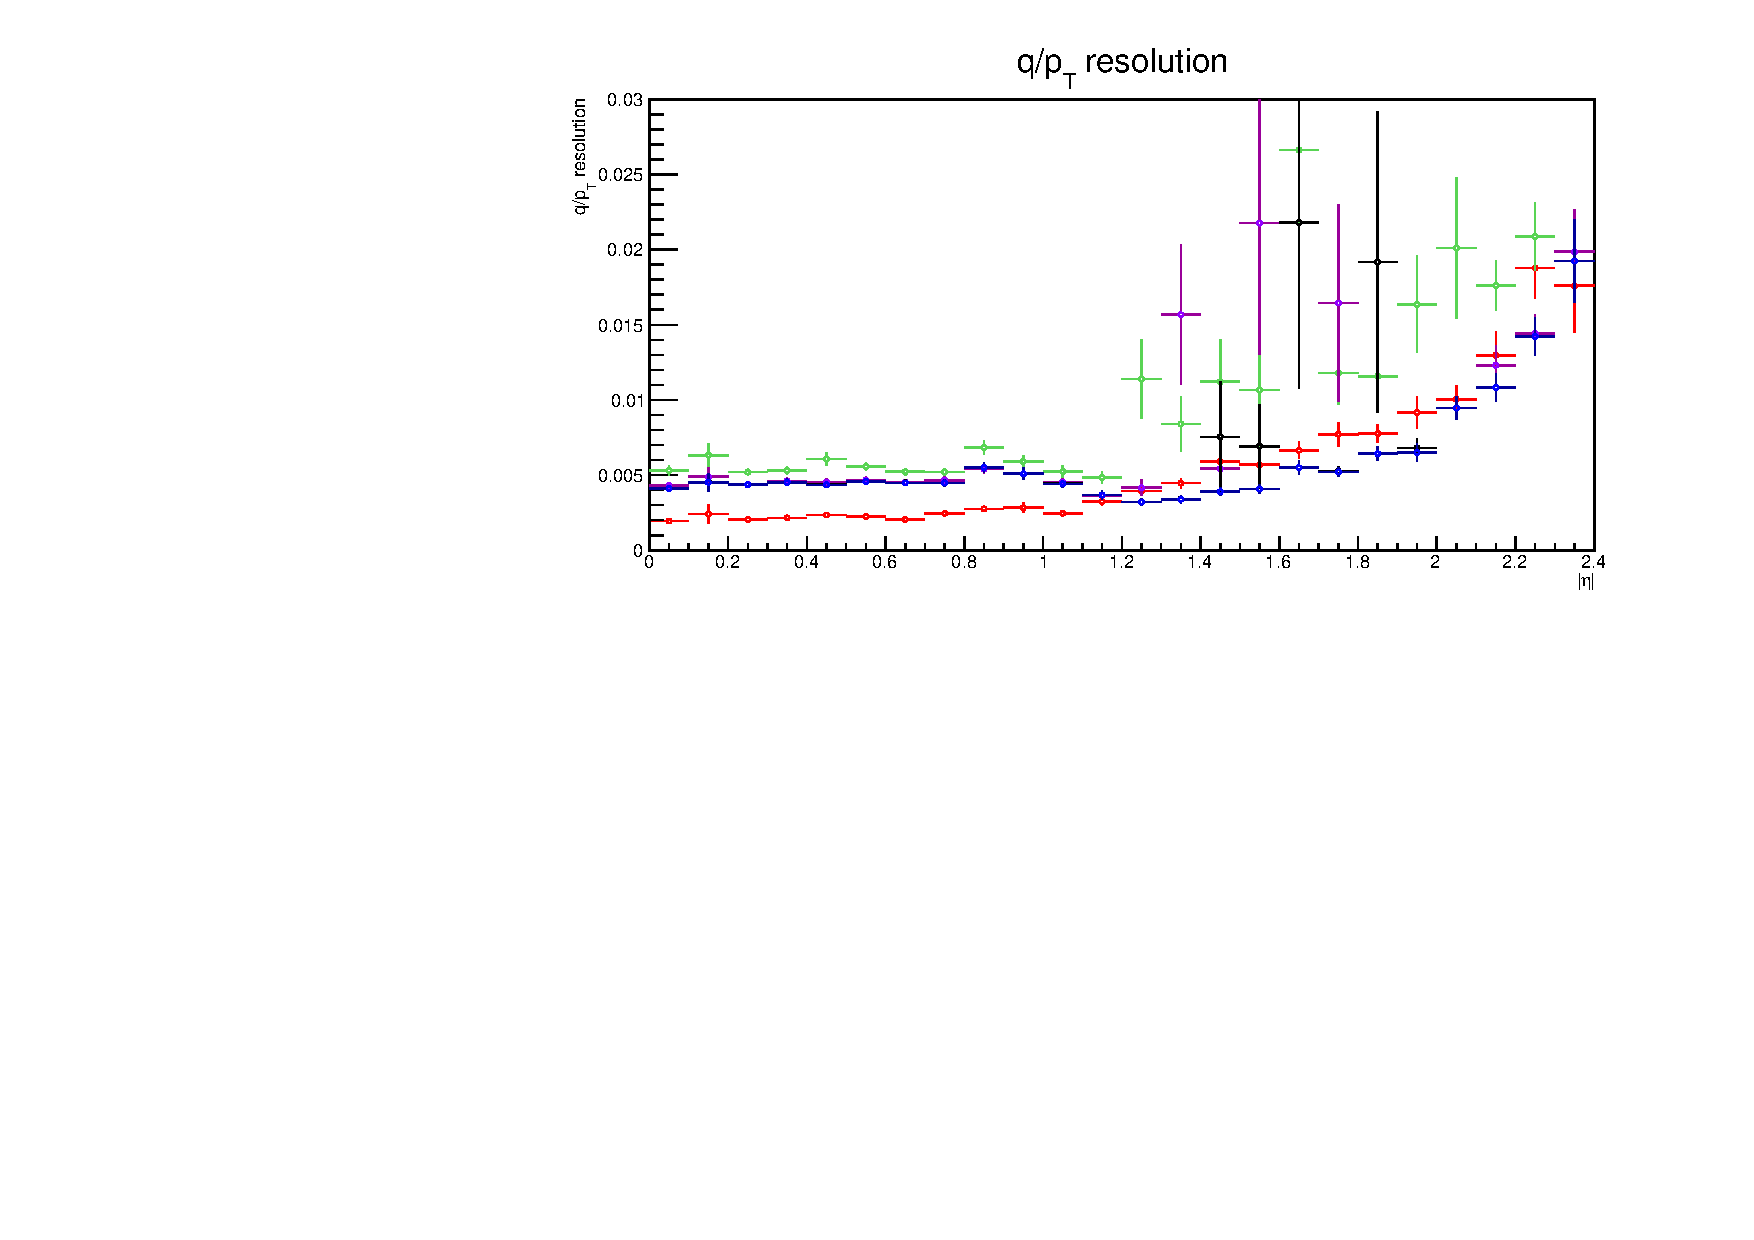
\includegraphics[width=0.47\textwidth]{figs/tk-upgrade/results-chi2fitter/qOverPtResVsEta_IterationComparison.pdf}
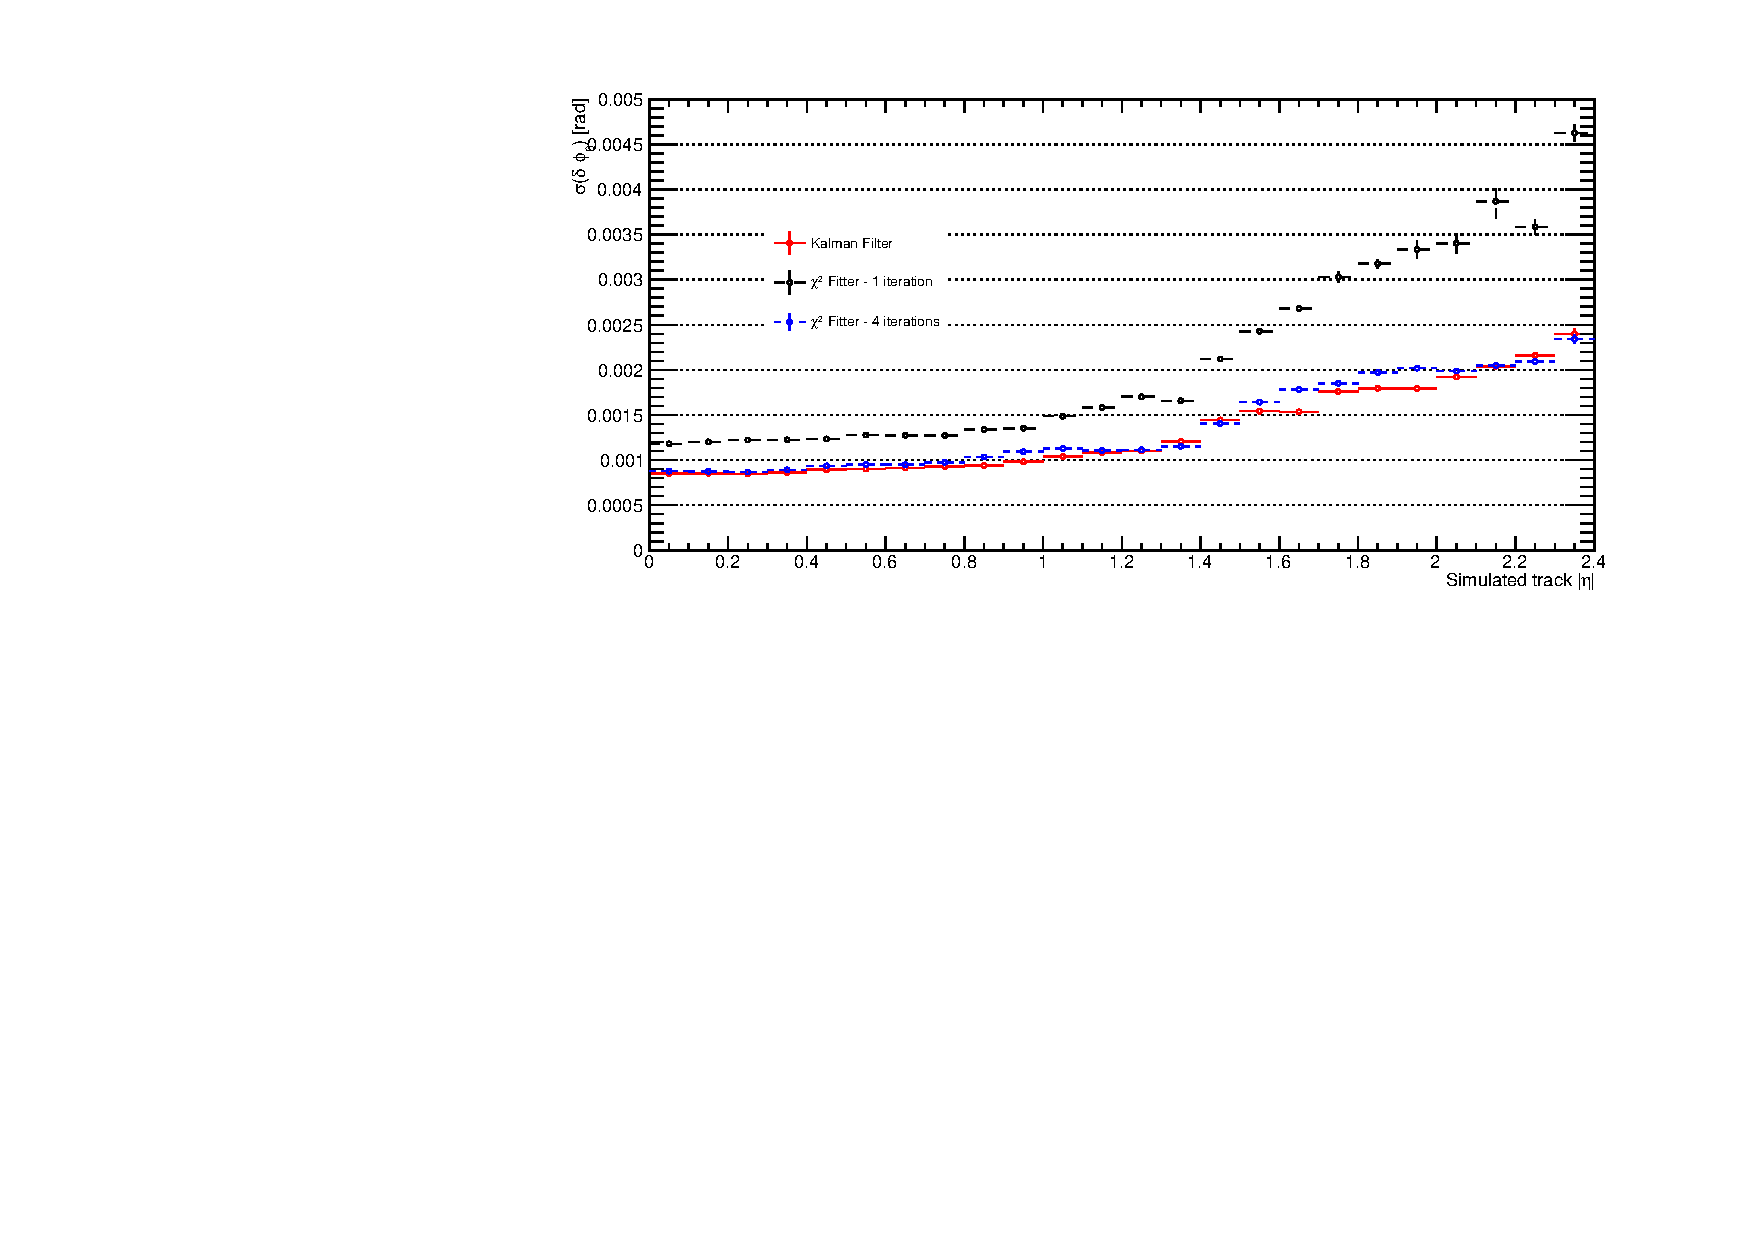
\includegraphics[width=0.47\textwidth]{figs/tk-upgrade/results-chi2fitter/phi0ResVsEta_IterationComparison.pdf}
\\
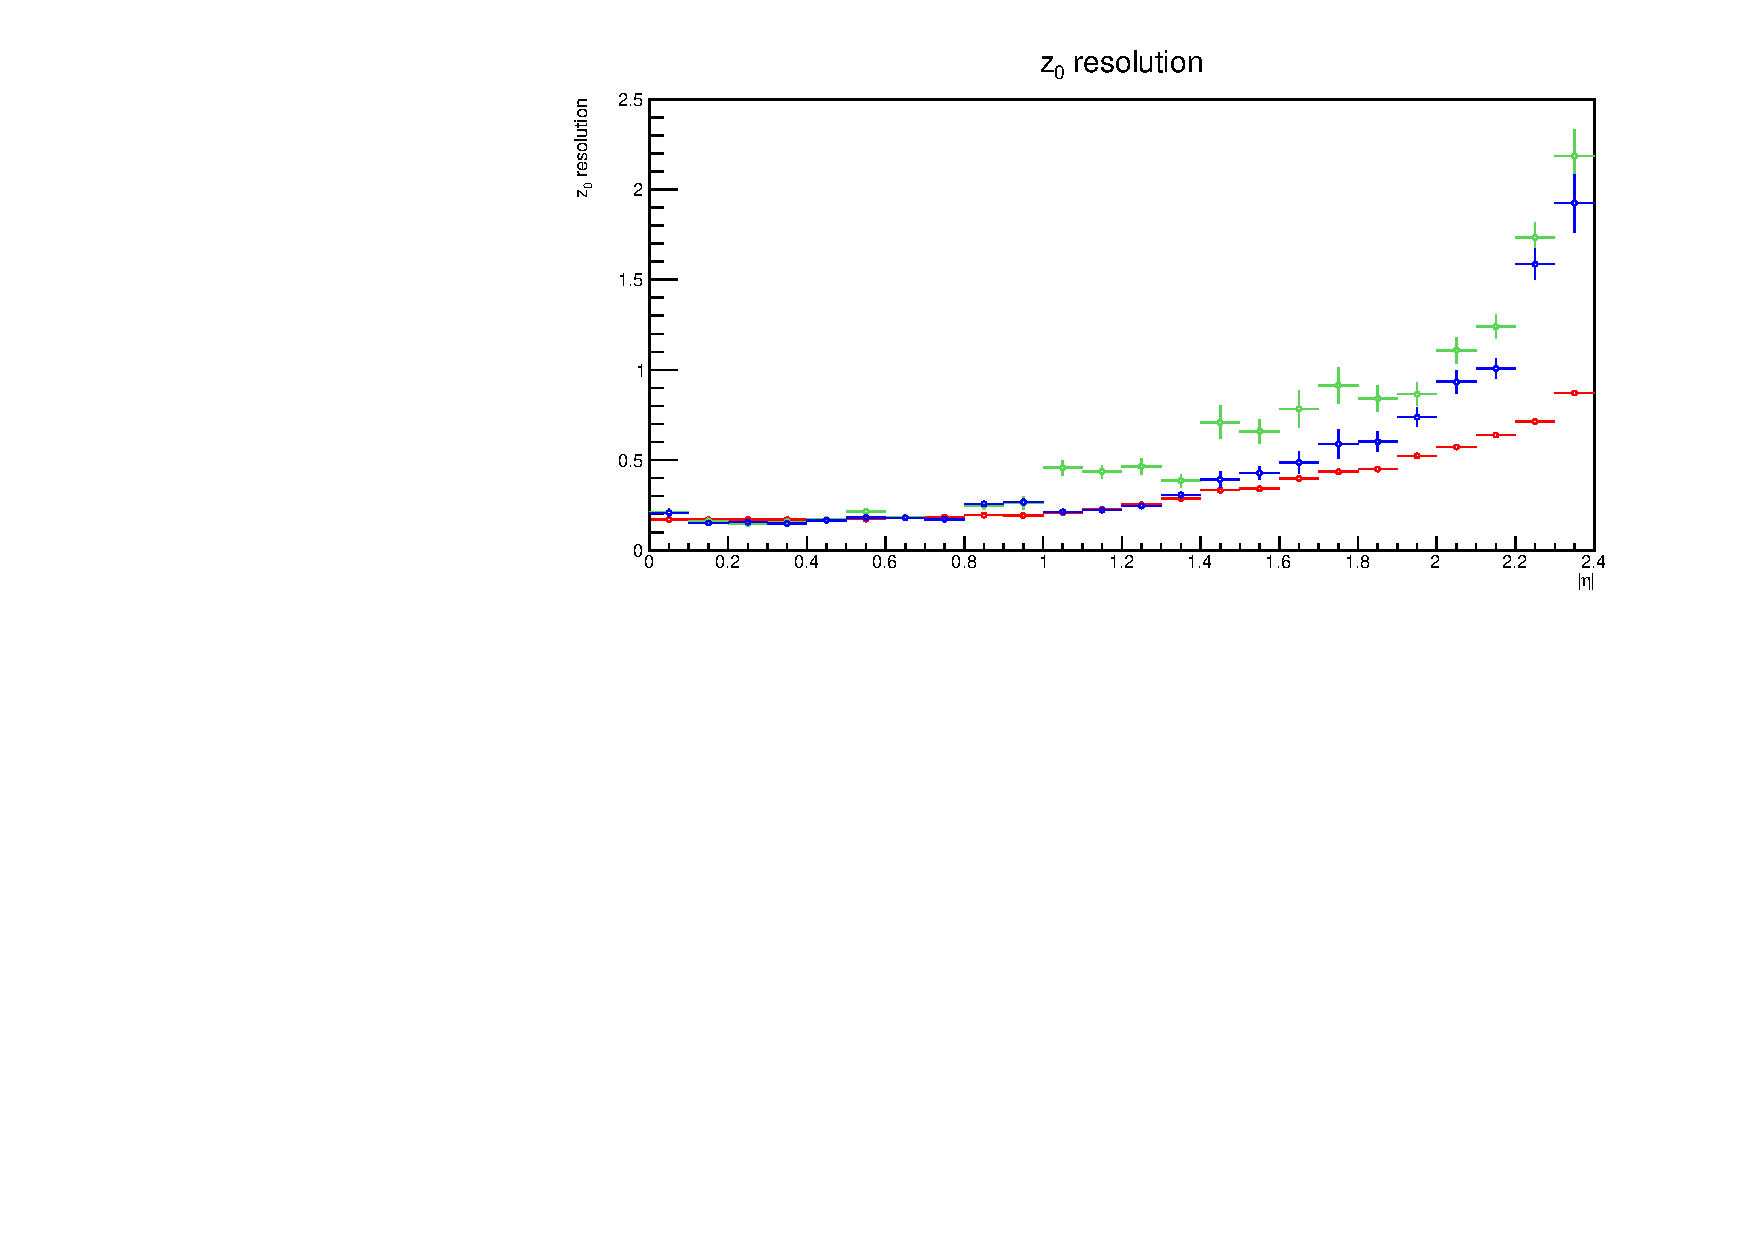
\includegraphics[width=0.47\textwidth]{figs/tk-upgrade/results-chi2fitter/z0ResVsEta_IterationComparison.pdf}
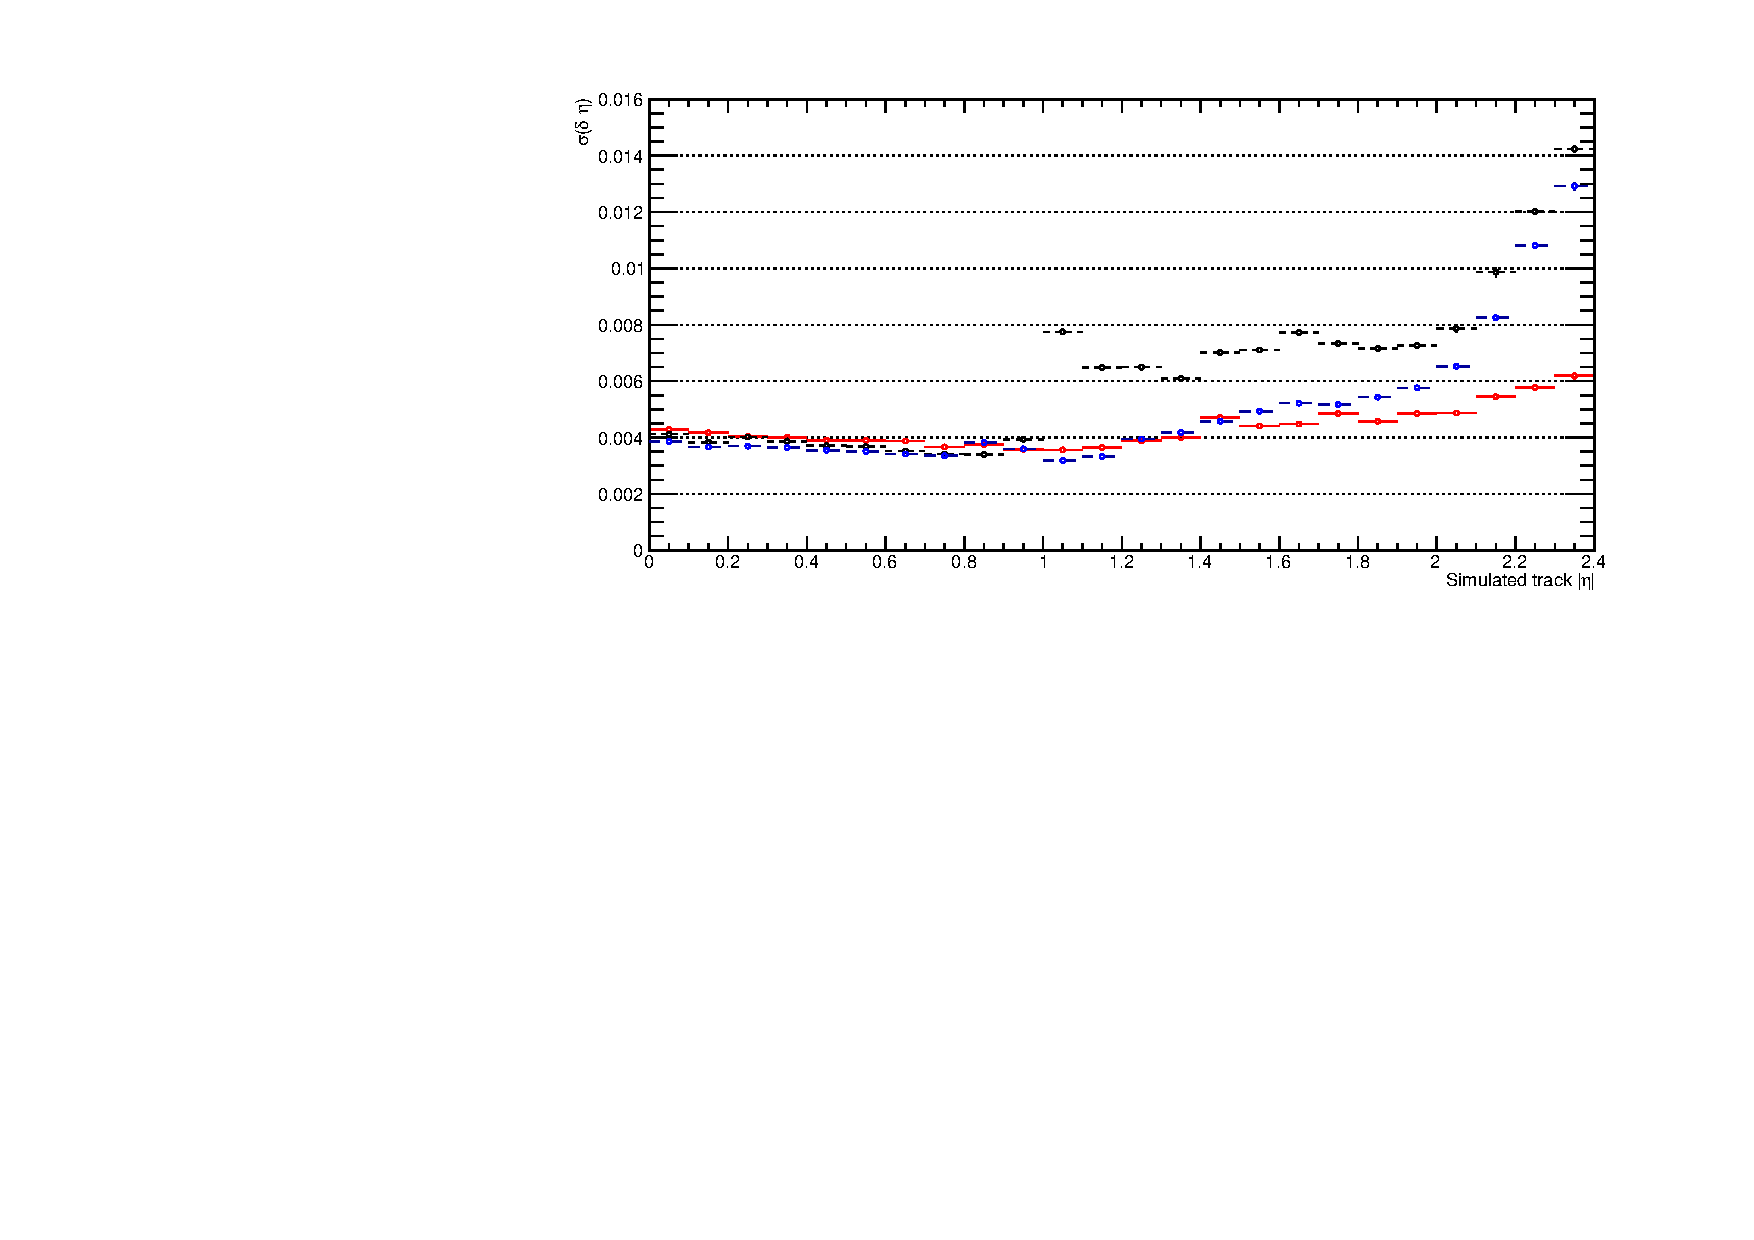
\includegraphics[width=0.47\textwidth]{figs/tk-upgrade/results-chi2fitter/etaResVsEta_IterationComparison.pdf}
\caption{
\pt resolution, $\phi$ resolution, $z_{0}$ resolution and $\eta$ resolution measured for primary reconstructed tracks in simulated \ttbar events at \PU of 200 for the approximated maths implementation of the linearised $\chi^{2}$ fit algorithm for one (green), two (purple), three (black) and four (blue) fitting iterations. The \KF (red) is also included for comparison.
\editComment{Make plots bigger!}
\editComment{Increase stats from 100!}
\editComment{Too cluttered perhaps?}
}
\label{fig:chi2HelixParametersResIterationsComparison}
\end{figure}

\subsubsection{Outlook}\label{subsubsec:chi2outlook}
Following the parallel development of both the linearised $\chi^{2}$ track fit and the \KF, it was decided that development on the former would be discontinued in favour of focussing resources on the latter.
The motivations behind this decision was that the \KF was capable of achieving a higher track finding efficiency with 100.0\% purity for matched tracks and considerable progress had been made with an implementation in firmware.
In contrast, the linearised $\chi^{2}$ track was not competitive in terms of track reconstruction ability, especially with respect to the stricter tracking efficiency definition, and there were also concerns over the potential feasibility of tabulating all (or the most frequently used) track derivatives in the endcap disks for FPGAs which were commercially available at the time.

\subsection{Tracking at low transverse momenta}\label{subsec:Tmtt2GeV}
The flexibility to reconstruct tracks down to a lower \pT threshold of 2\GeV may be desirable if the trigger requirements demand it and the impact of this potential requirement on the proposed proposed track-finder system was studied.
These studies were initially undertaken as part of the the robustness studies required for the December 2016 demonstrator review, focussing on recovering tracking efficiency below 3\GeV with the \HT, and were subsequently built upon with modifications to the \KF algorithm after 2016.
The results relating to \HT modifications were produced prior to the conclusion of the demonstrator review and were produced using the flat barrel geometry, and the results for the \KF improvements produced with the tilted barrel geometry.

\subsubsection{Hough Transform Optimisation}\label{subsubsec:lowPtOptHT}
Lowering the \HT \pT threshold from 3\GeV to 2\GeV required modifying the GP and HT configuration parameters to ensure adequate duplication in $\phi$ and increasing the number of the \qpt columns by 50\% to take into account the increased \pt range whilst maintaining the same precision, respectively.
The increased number of \qpt columns has the impact of increasing the required FPGA resources by 50\% and the output data rate from the \HT by a factor of 2.2.

Without any further modifications, there is a considerable degradation in the track reconstruction efficiency by the \HT in the range $2 < \pt < 2.7$\GeVc, due to these low momentum tracks being dominated by multiple scattering.
This results in stubs not always intersecting within a single \HT cell and thus failing to exceed the threshold criteria and generate track candidates.
To mitigate against such track reconstruction efficiency losses, using a preexisting feature which had been separately implemented in firmware, the precision of the \HT cells along \qpt and $\phi_{T}$ for the range $2 < \pt < 2.7$\GeVc was reduced by a factor of two (\ie $2 \times 2$ cells were merged).
Additionally, the \KF state $\chi^2$ cuts for this low \pT range were optimised to reflect the increased hit position uncertainty resulting from the decreased precision of the hits in these \HT cells and thus reduce the number of duplicate and fake tracks as far as possible without impacting on the \HT track reconstruction efficiency.
Figure~\ref{fig:2GeVFlatEff} shows how the tracking efficiency improves following the use of the variable precision \HT with and without optimised \KF state cuts after both the \HT and the full demonstrator chain. 

\begin{figure}[tbp]
\centering
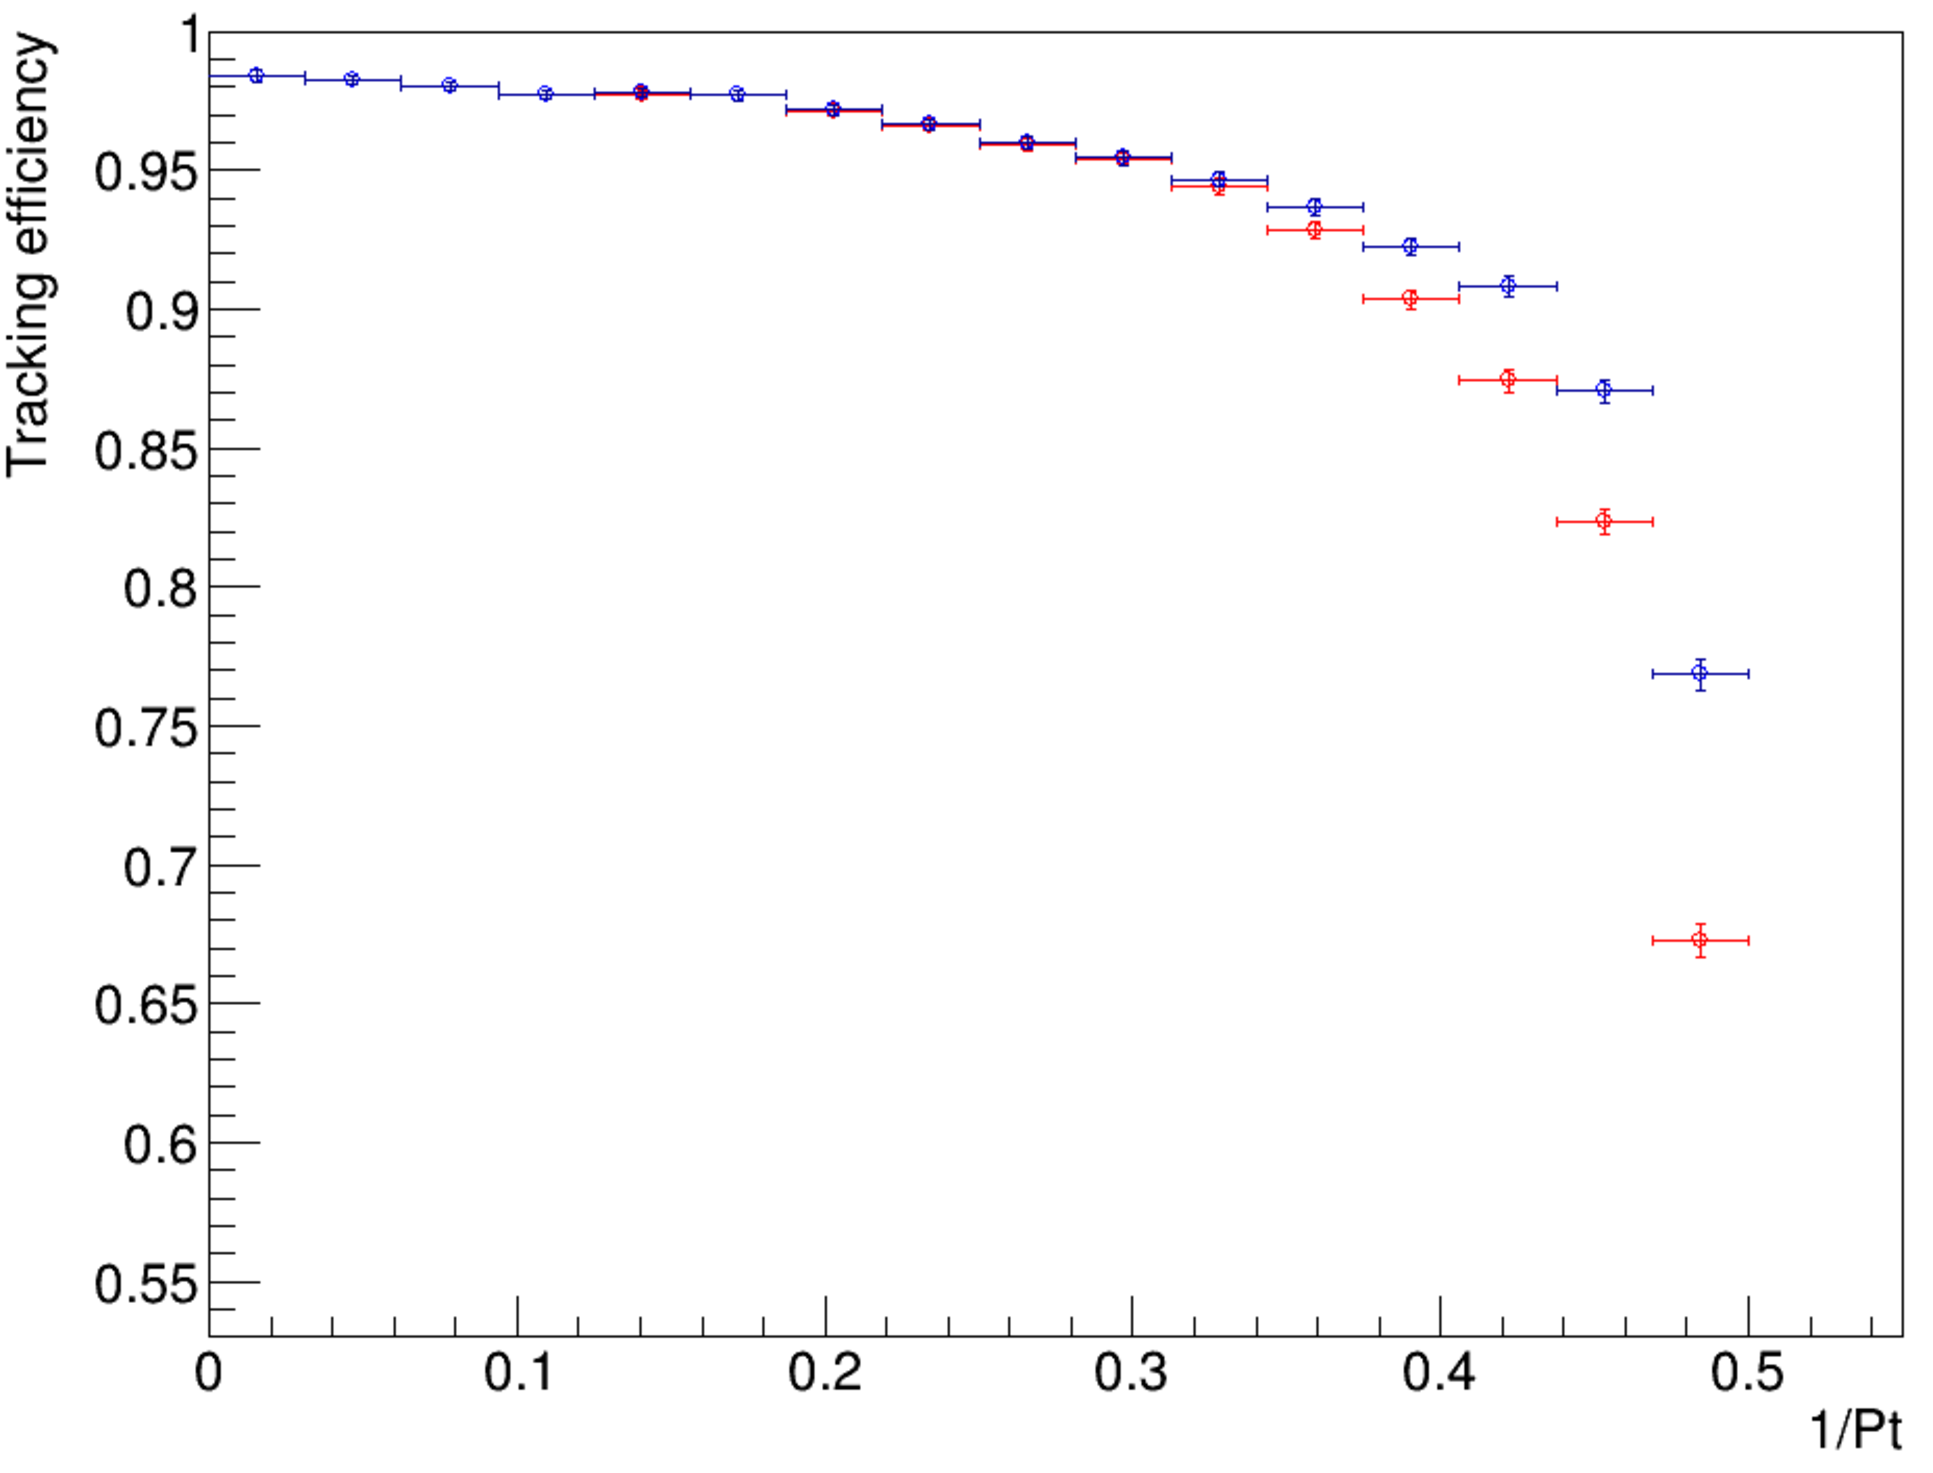
\includegraphics[width=0.47\textwidth]{figs/tk-upgrade/results-lowPtTracking/htTrackingEffVsInvPtFlatGeometry_5000.pdf}
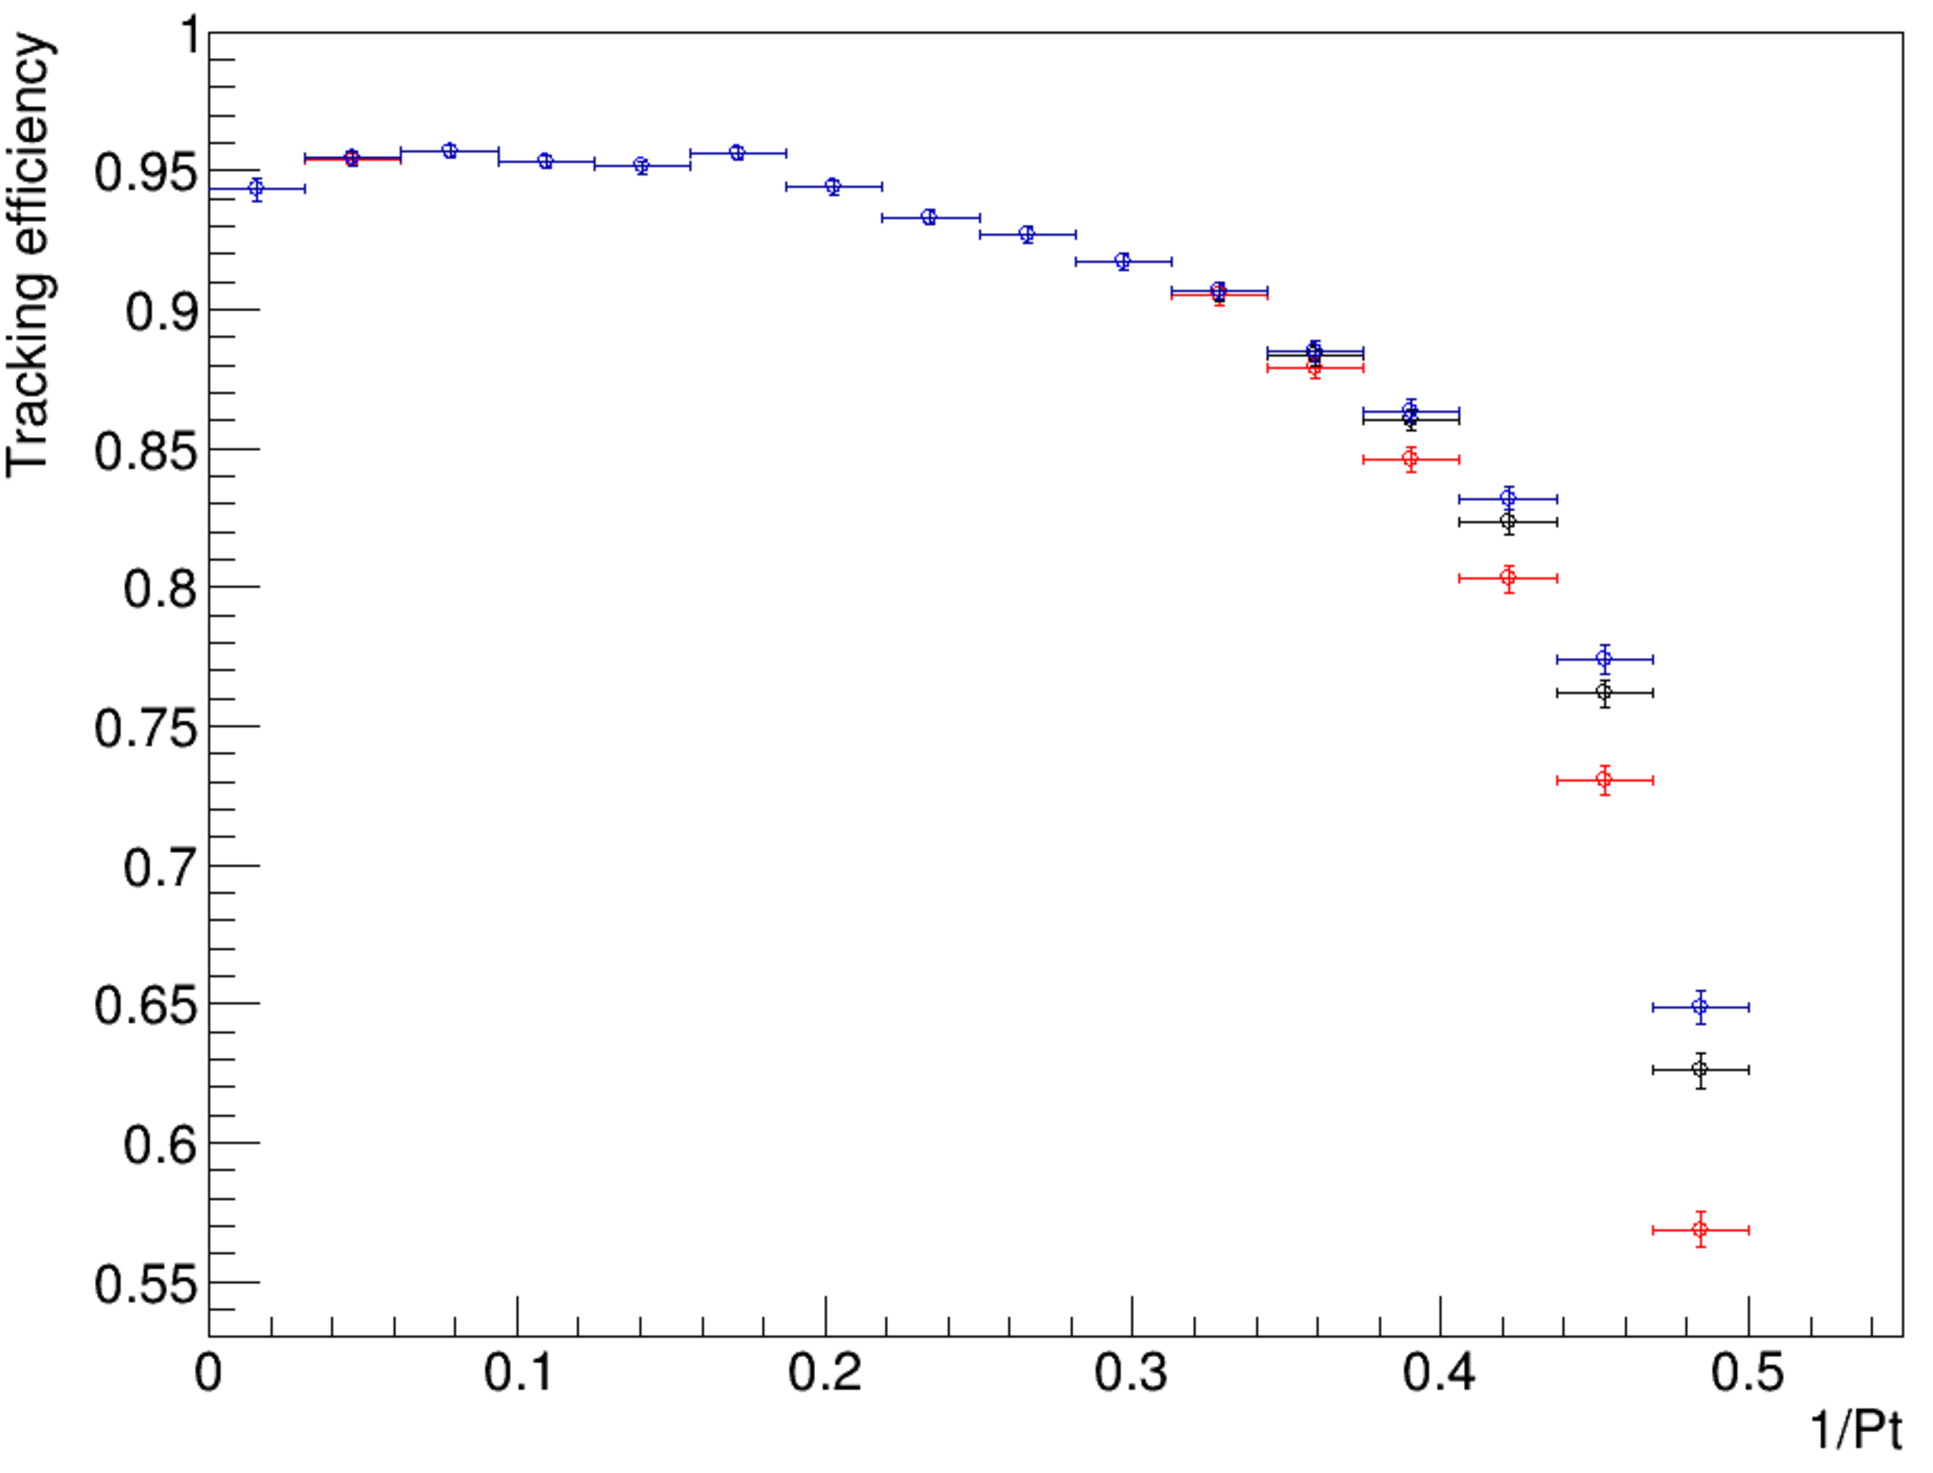
\includegraphics[width=0.47\textwidth]{figs/tk-upgrade/results-lowPtTracking/kfTrackingEffVsInvPtFlatGeometry_5000.pdf}
\caption{Plots post-\HT (left) and post-\KF (right) showing tracking efficiency in low pT range with only the number of \qpt columns increased (red) and with the increased number of columns, HT cell merging and \KF state cuts optimisation(blue) for \ttbar events at \PU of 200.
\editComment{Plots require legend and removal of black coloured data points!}
}
\label{fig:2GeVFlatEff}	
\end{figure}

%%% Disucss table here
Table~\ref{tab:trackFindingPerformance2GeVHT} shows the impact that the decreased precision \HT cells and optimised \KF state cuts have on tracking performance both following the \HT and the full chain.
It is clear that whilst the merging of adjacent \HT cells recovers  tracks which did not previously intersect within a single \HT cell, the tracking efficiency following the full chain is significantly less than that post-\HT.
As shown in Figure~\ref{fig:2GeVFlatEff}, these losses occur for tracks where the particle's transverse momenta is less than 3\GeV, as the \KF does not take the effects of \MS into account.
This shortcoming of the \KF also accounts for it not being as efficient at removing fake tracks, with an observed increase of 5\% in the fraction of fakes reconstructed.
The duplicate removal algorithm however, remains effective at removing almost all the duplicates.

\begin{table}[htbp]
\topcaption {Track finding performance on simulated \ttbar events at a \PU of 200, after the \HT and the full chain  for the configurations of only increasing the number of \qpt columns (\emph{Default}), additionally using \HT cell merging and the optimised \KF state cuts (\emph{Optimised}).
The track finding efficiencies following each stage are given using the efficiency definitions given in Chapter~\ref{subsubsec:helixParameter}, along with the mean number of tracks and the fraction of those tracks which are either fake or duplicate tracks.
\editComment{better to quote non-integer numbers and fractions of duplicates/fakes?}.
\editComment{Ermm ... get table to fit onto page!}
}
\label{tab:trackFindingPerformance2GeVHT}
  \centering
% This increases column spacing.
  \addtolength{\tabcolsep}{1ex}
% This right-aligns numbers in column, but centers them under column title.
  \begin{tabular}{ccr@{\hspace{4ex}}r@{\hspace{4ex}}r@{\hspace{4ex}}r@{\hspace{4ex}}r@{\hspace{4ex}}r@{\hspace{4ex}}}
   \hline
   \bf{Configuration} & \bf{Stage} & \bf{Efficiency [\%]} & \multicolumn{1}{r}{\bf{Mean \# of tracks}} & \multicolumn{1}{r}{\bf{\% of fakes}} & \multicolumn{1}{r}{\bf{\% of duplicates}}  \\
        \hline
    Default & \bf{HT}     & 93.6 & 713.2 & 34.0 & 44.5 \\  
    & \bf{Full chain}     & 89.2 & 193.9 & 21.1 & 5.1 \\      
%   \hline
%    Merge & \bf{HT}     & 94.6 & 799.2 & 40.5 & 39.7 \\  
%    & \bf{Full chain}     & 89.8 & 206.5 & 25.4 & 3.9 \\      
    \hline
    Optimised & \bf{HT}     & 94.6 & 799.2 & 40.5 & 39.7 \\  
    & \bf{Full chain}     & 90.0 & 210.4 & 26.3 & 3.8 \\      
   \hline
   
 \end{tabular}
 \addtolength{\tabcolsep}{-1ex}
\end{table}

The point made about \MS not being properly accounted for in the \KF is nicey illustrated by figure ~\ref{fig:2GeVFlatChi2Ndf} which shows the distributions of $\chi^{2} \div \text{number of degrees of freedom}$ ($\frac{\chi^{2}}{ndf}$) as a function of $\frac{1}{\pT}$ in figure~\ref{fig:2GeVFlatChi2Ndf} for genuine tracks produced by the \KF.
If all uncertainties were accounted for, the ideal distribution of $\frac{\chi^{2}}{ndf}$ would be unity for all \pT, in contrast to the dramatic increase above approximately 3\GeV from the approximately flat distribution at order unity.

\begin{figure}[tbp]
\centering
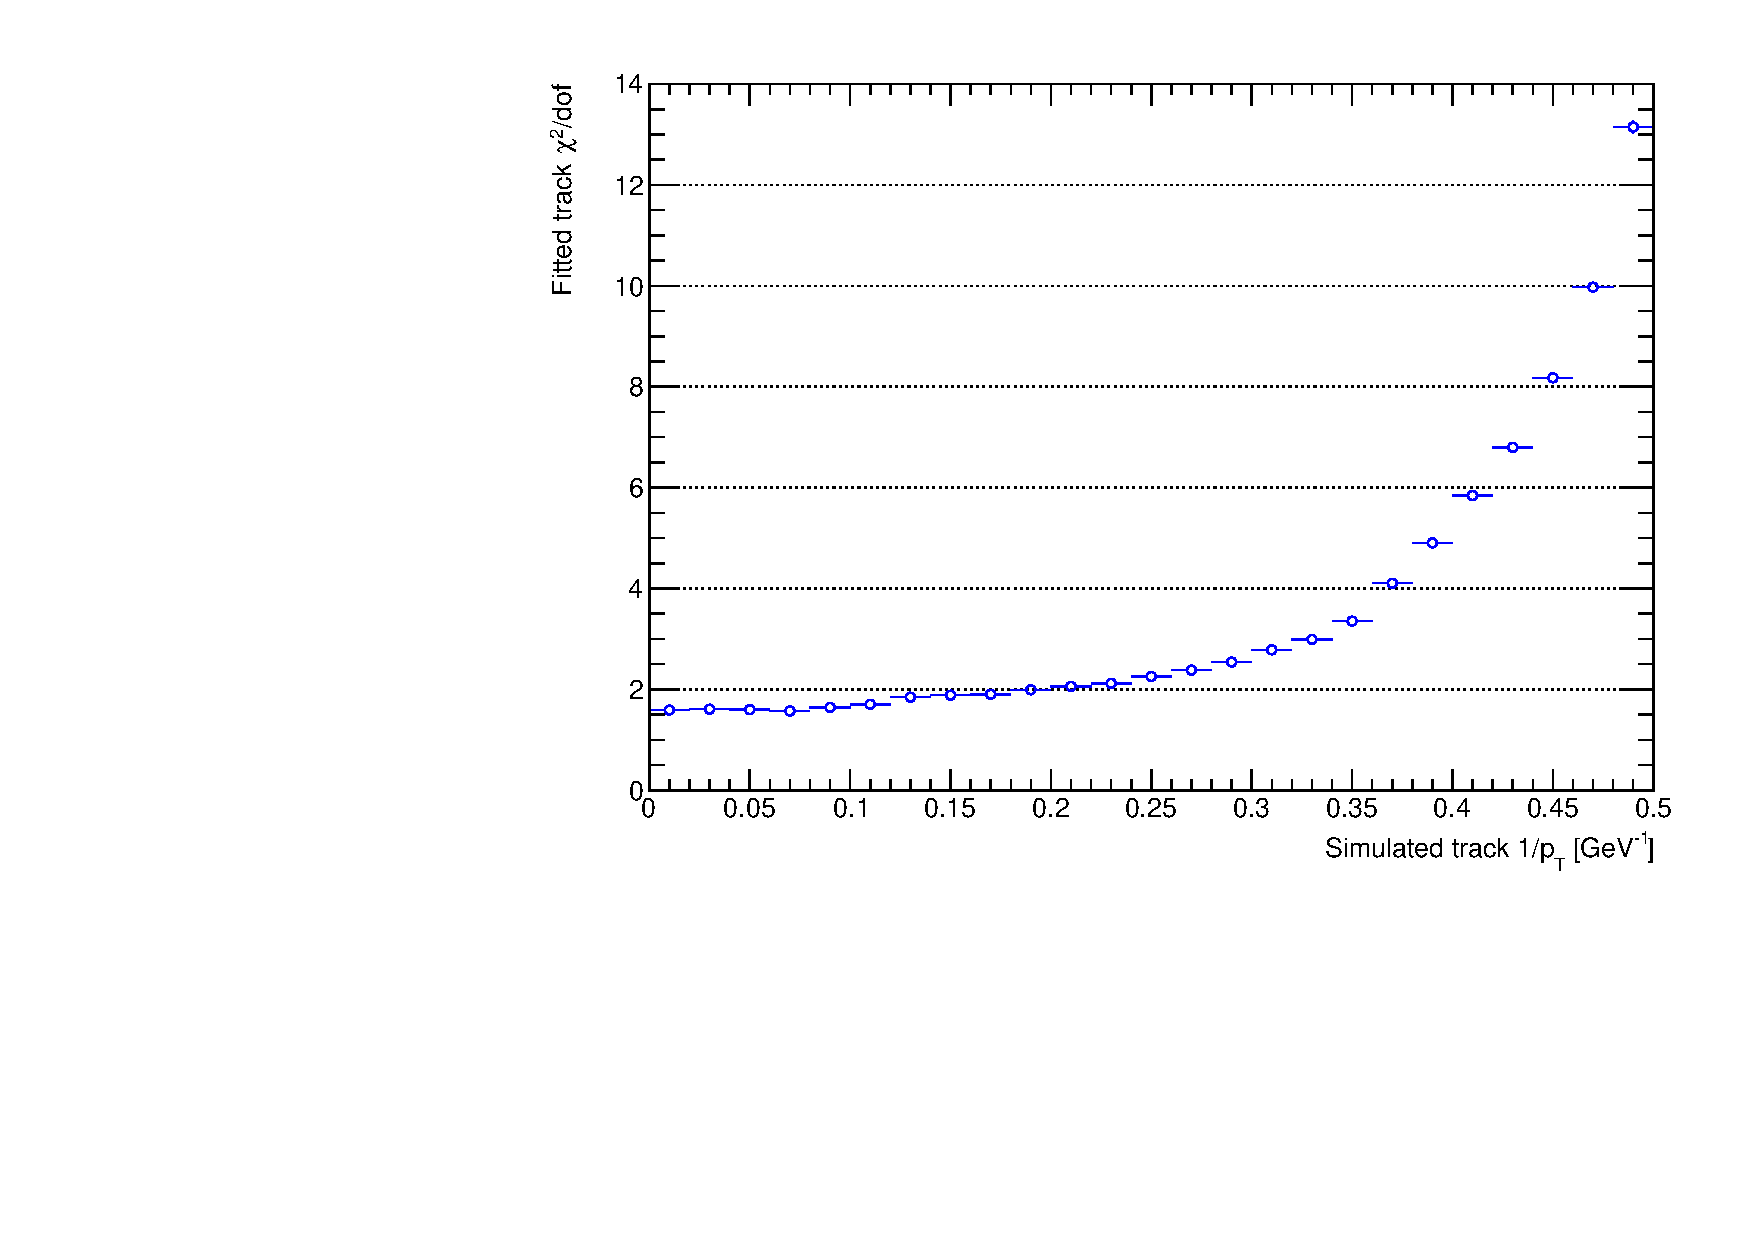
\includegraphics[width=\textwidth]{figs/tk-upgrade/results-lowPtTracking/kfChi2NdfVsInvPtFlatGeometry_5000.pdf}
\caption{Plot of $\frac{\chi^{2}}{ndf}$ as a function of $\frac{1}{\pT}$ for genuine tracks produced by the \KF.}
\label{fig:2GeVFlatChi2Ndf}
\end{figure}

%% Discuss the resolution plots here
Figure~\ref{fig:htHelixParametersResVsInvPt} shows the resolutions of the track parameters as a function of transverse momenta in simulation for tracks originating from the primary interaction in \ttbar events at \PU of 200 following fitting by the \KF for both before and after optimising the \HT for tracking at low transverse momenta.
The resolutions are comparable for $\pT < 3\GeV$, with slight a degradation in the $\phi_{0}$ resulting from the decreased precision coordinates from the \HT and small improvements in the $z_{0}$ resolution due to decreased precision \HT reconstructing more correct stubs, which provides the \KF with more (and potentially better) stubs to chose from during the filtering and fitting process.

\begin{figure}[htb]
\centering
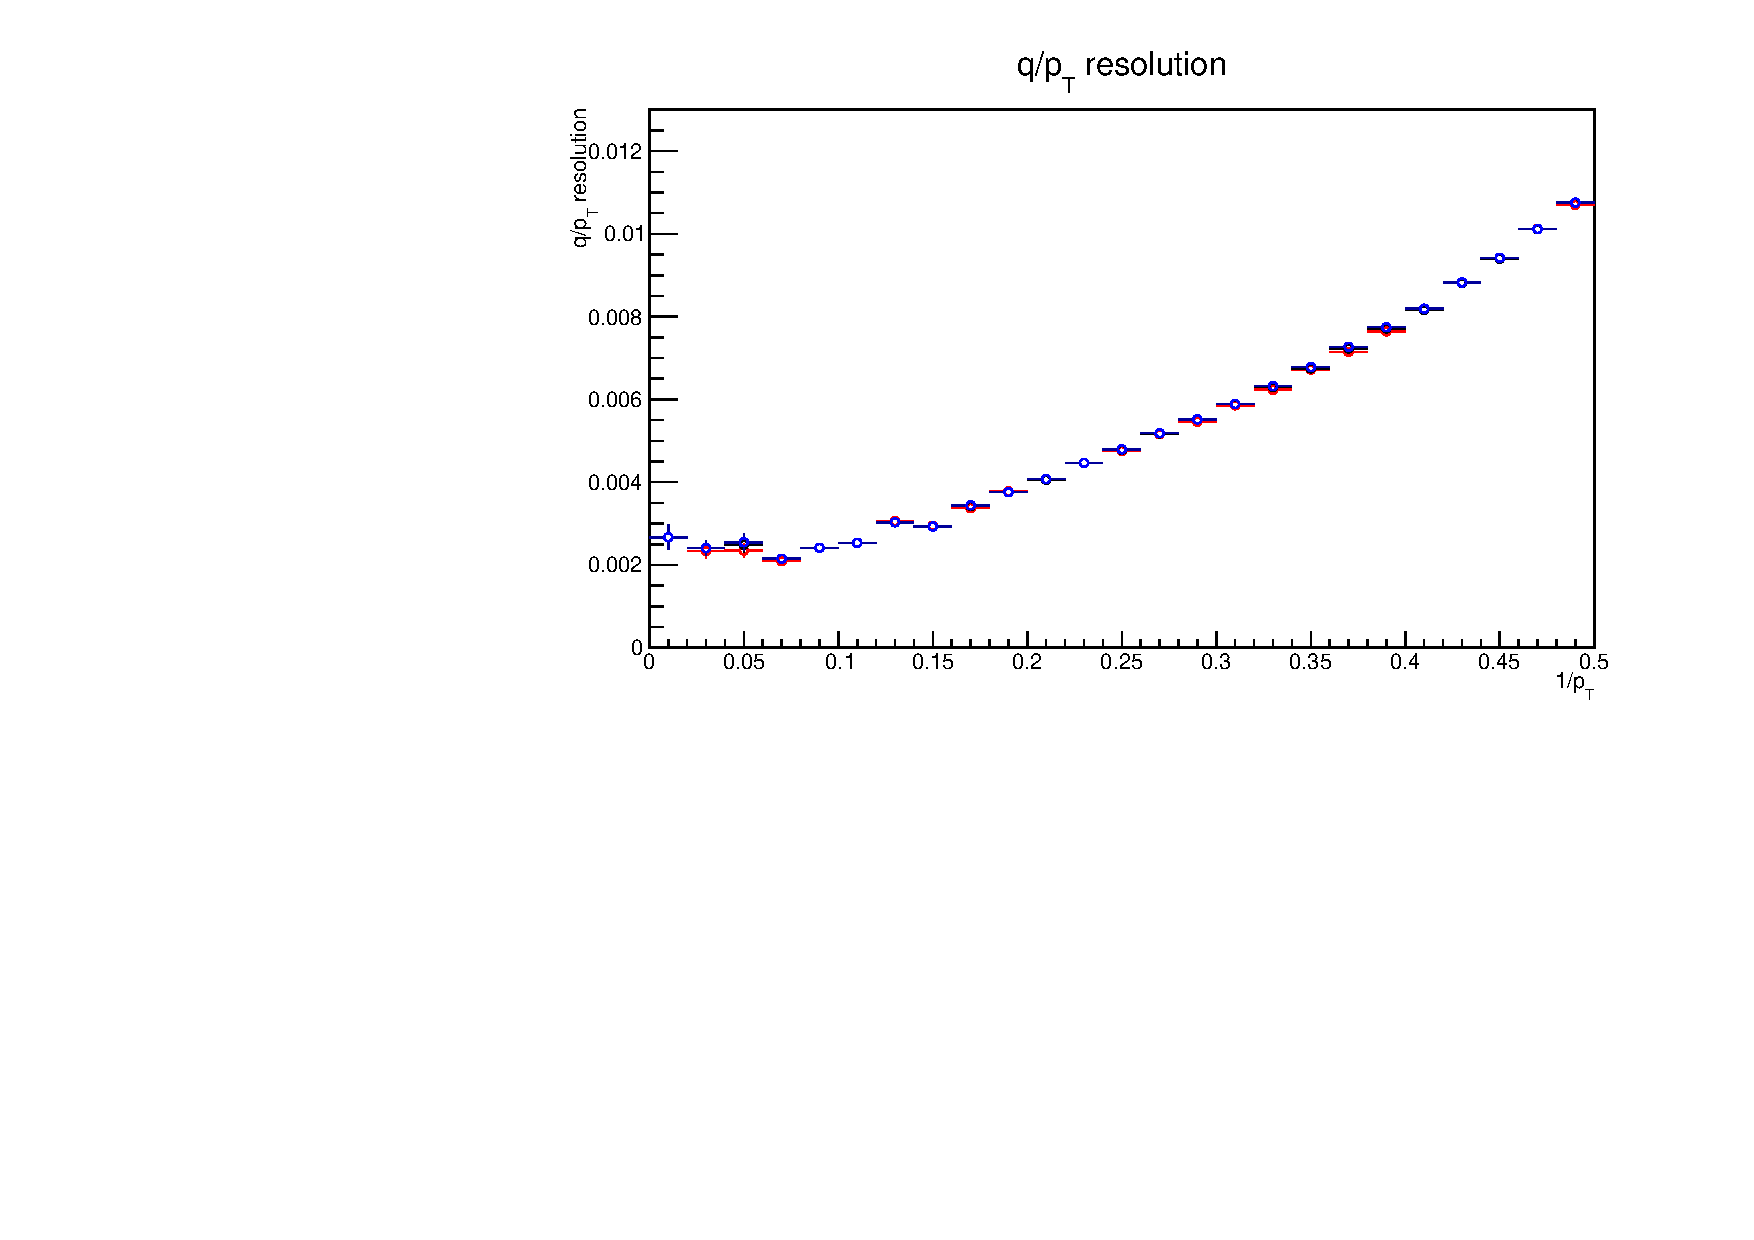
\includegraphics[width=0.47\textwidth]{figs/tk-upgrade/results-lowPtTracking/qOverPtResVsInvPtFlatGeometry_5000.pdf}
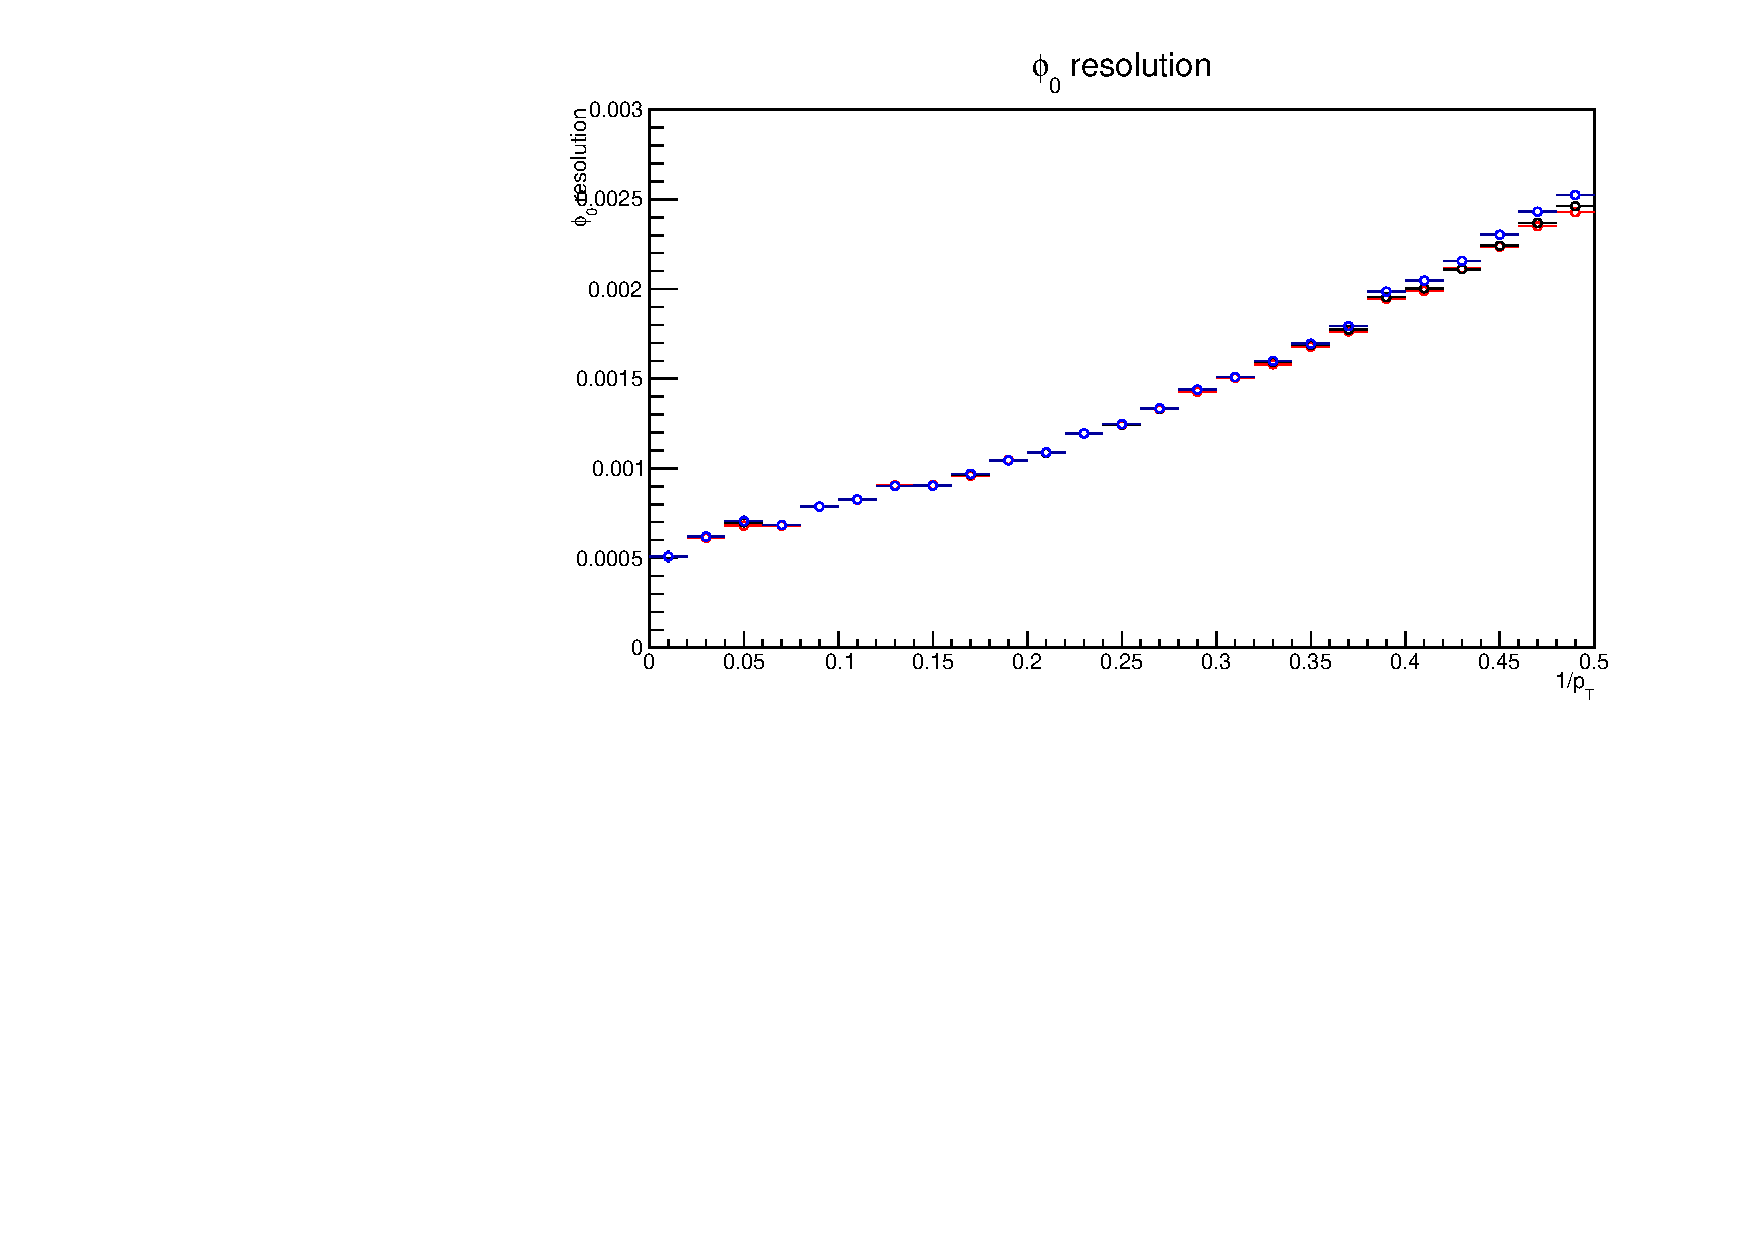
\includegraphics[width=0.47\textwidth]{figs/tk-upgrade/results-lowPtTracking/phi0ResVsInvPtFlatGeometry_5000.pdf}
\\
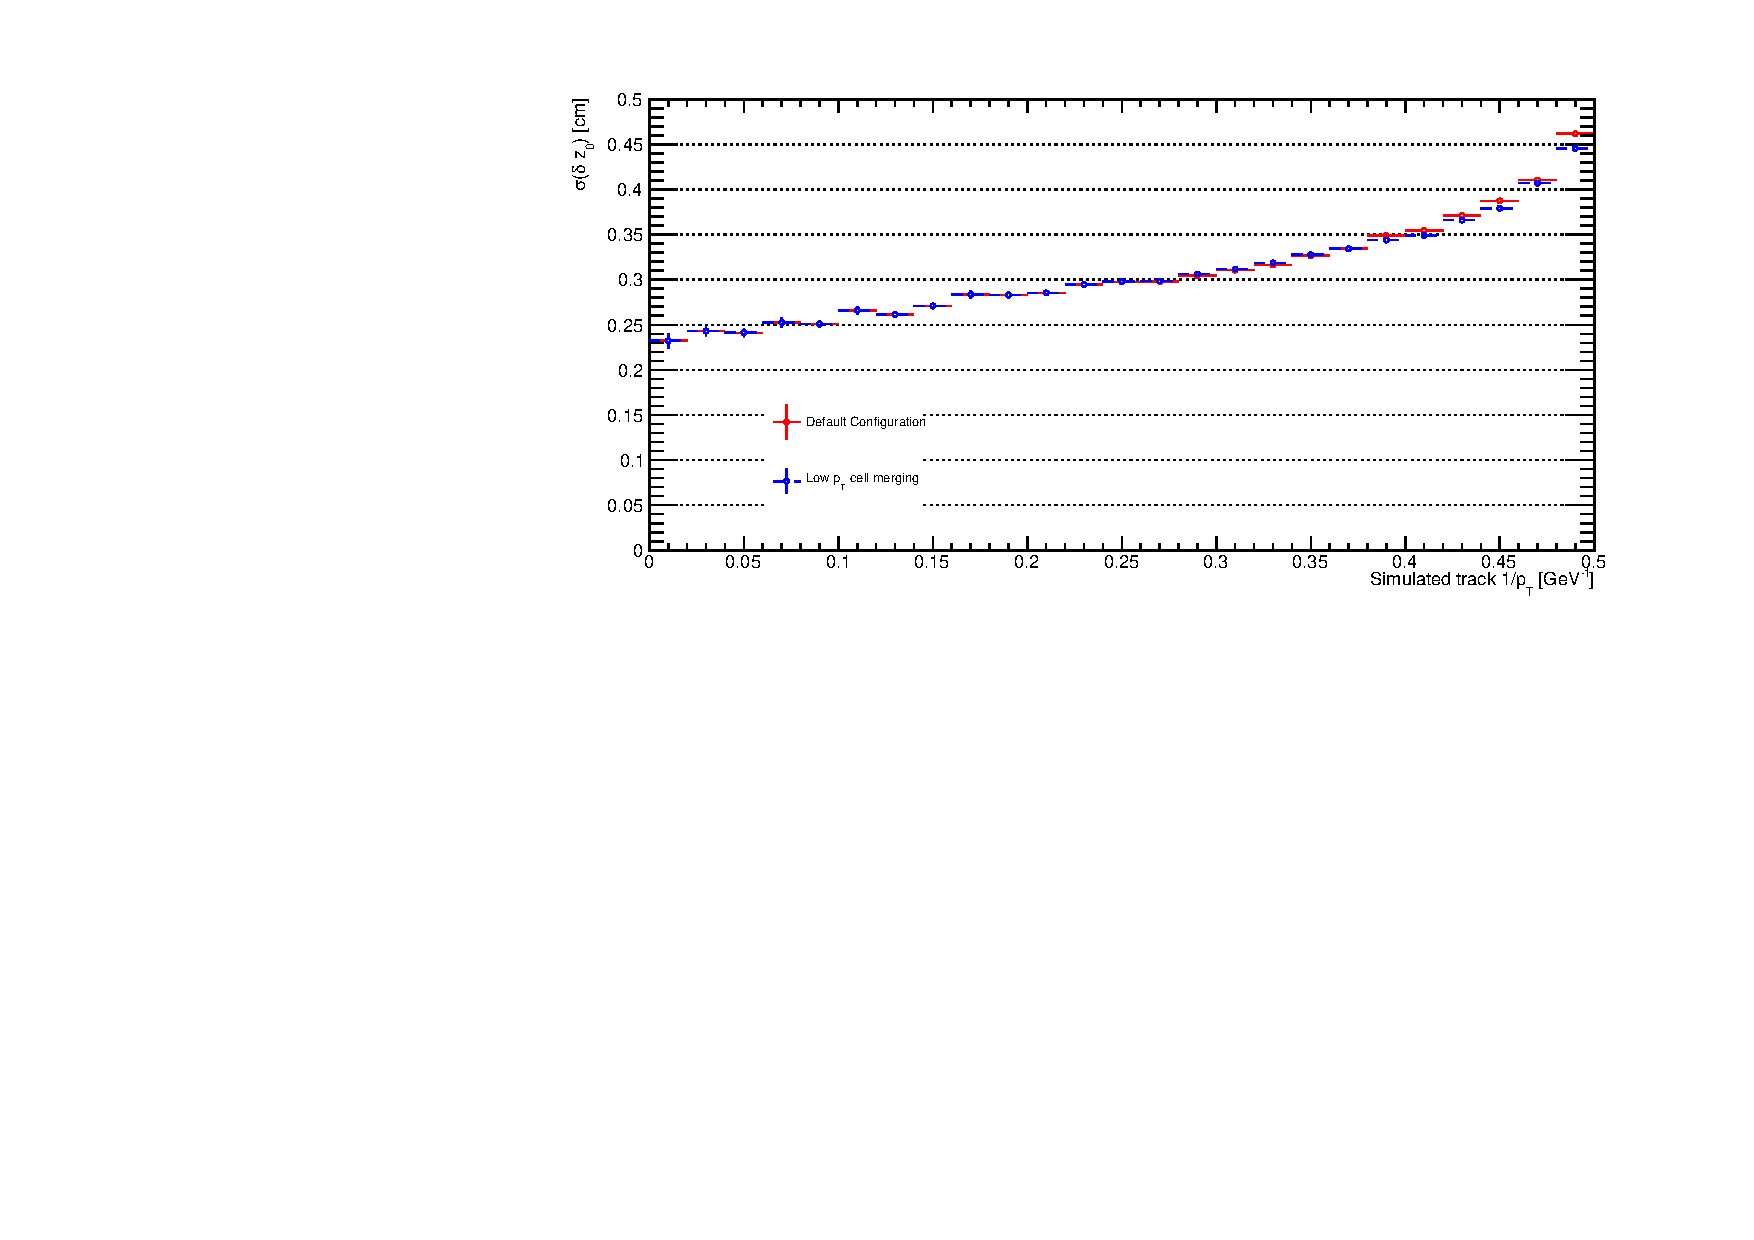
\includegraphics[width=0.47\textwidth]{figs/tk-upgrade/results-lowPtTracking/z0ResVsInvPtFlatGeometry_5000.pdf}
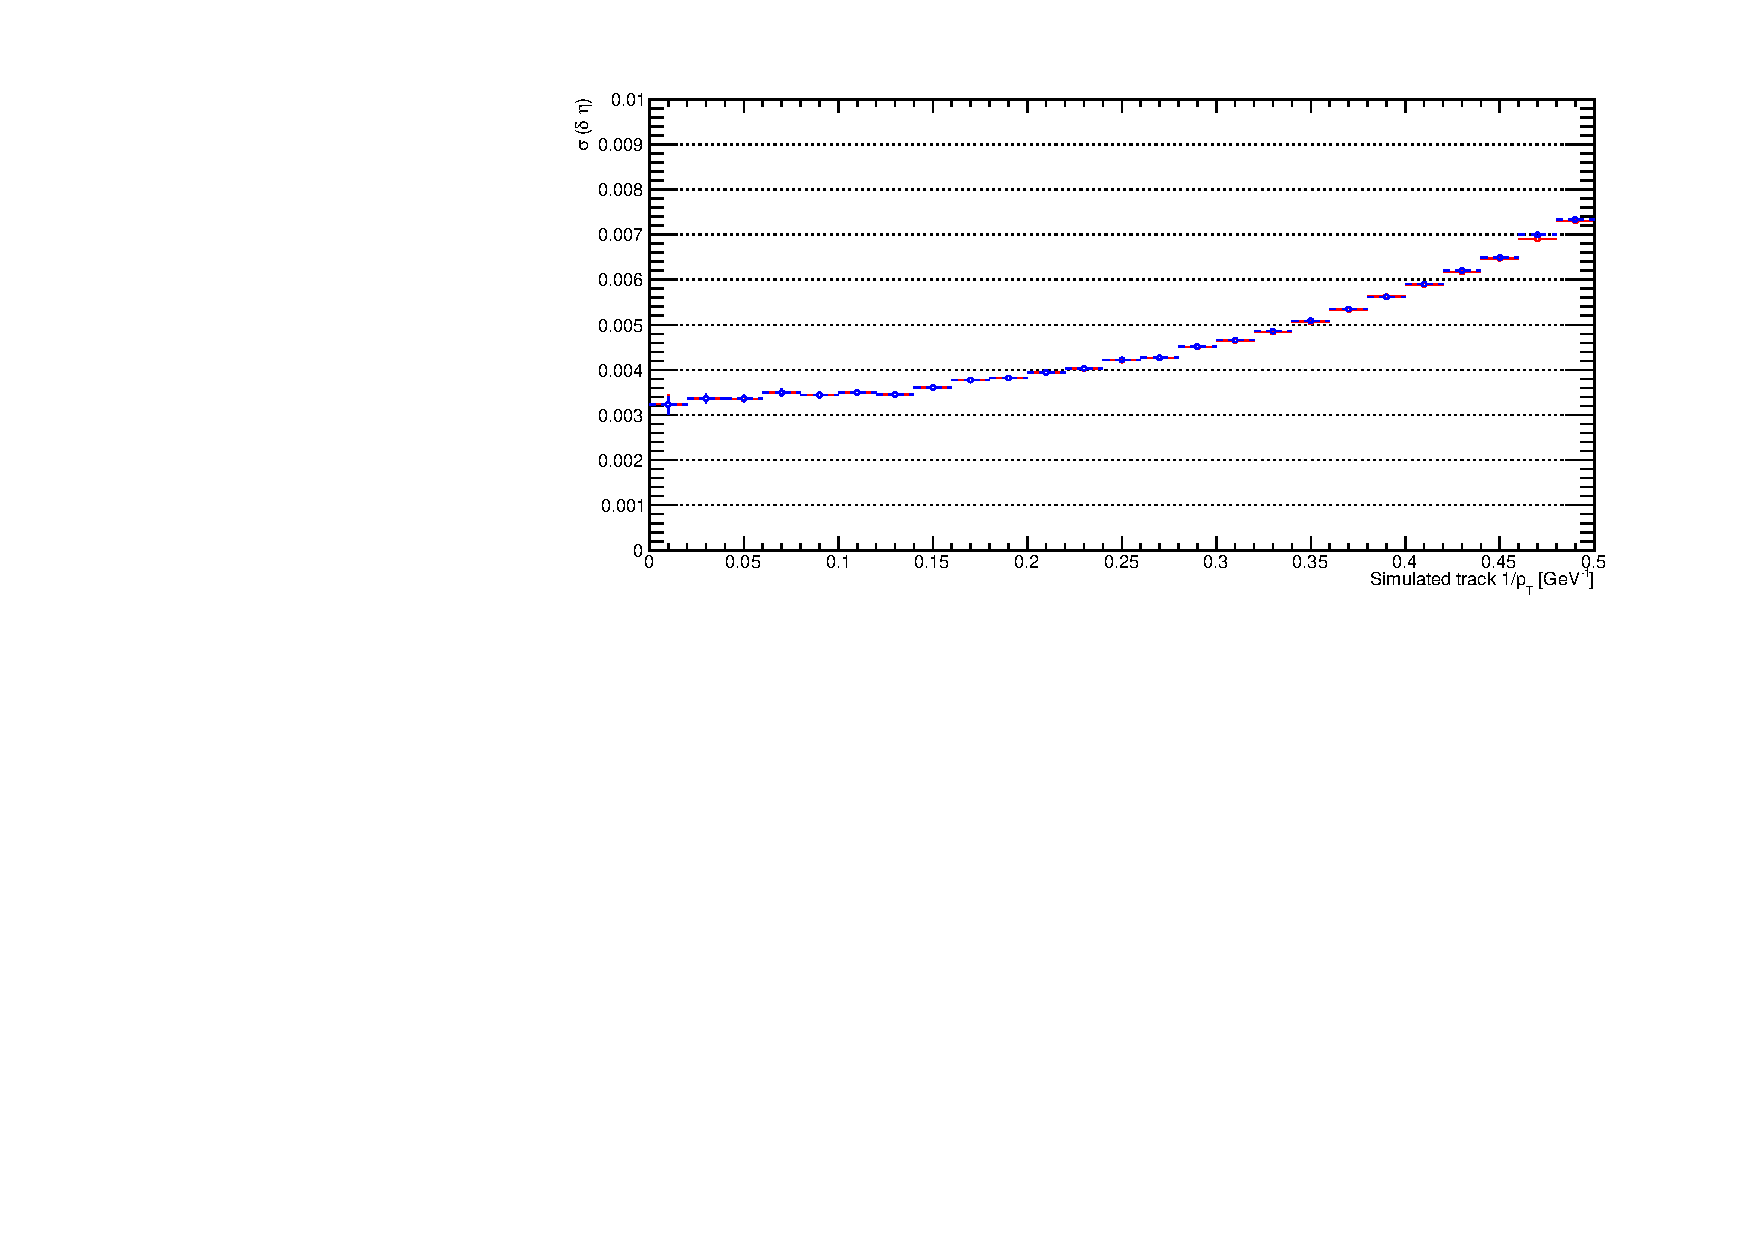
\includegraphics[width=0.47\textwidth]{figs/tk-upgrade/results-lowPtTracking/etaResVsInvPtFlatGeometry_5000.pdf}
\caption{
\pt resolution, $\phi$ resolution, $z_{0}$ resolution and $\eta$ resolution measured for primary reconstructed tracks in simulated \ttbar events at \PU of 200.
\editComment{Make plots bigger!}
\editComment{Best to express resolution in terms of $\pT$ or $\frac{1}{\pT}$?}
}
\label{fig:htHelixParametersResVsInvPt}
\end{figure}

\subsubsection{Kalman Filter Optimisation}\label{subsubsec:lowPtOptKF}
\editComment{Plan to use these emph phrases in the revised KF section above}
Incorporation of \MS into the \KF involved including a \emph{process noise} term, namely the variance of the multiple scattering angles, to the \emph{measurement noise} (\ie measurement error) term already present in the \KF covariance matrix.
In this updated form, the \KF now can consider stubs which are compatible with those that have undergone \MS, allowing tracks with previously discarded stubs to be reconstructed and the resultant more accurate $\chi^{2}$ values that can be used to better discriminate against fake track states.

For small deflection angles and relativistic particles, $\sigma_{\theta}$ for a each layer is given by~\cite{Lynch:1990sq}~:

\begin{equation}
\sigma_{\theta} = \frac{13.6\MeV}{\beta c p} q \sqrt{\frac{x}{X_{0}}} [1 + 0.088 \log_{10}{\frac{x}{X_{0}}}]  \;
\label{eq:scatter1}
\end{equation}

where, the momentum, velocity, electrical charge of the incident particle and thickness of the scattering medium in radiation lengths are given by $p$, $\beta c$, $q$ and $\frac{x}{X_{0}}$ respectively and the result being good to better than 11\%.

With the particles involved having relativistic velocities (\ie $\beta c \cong 1$) and scattering in the r-z plane ignored as the impact of multiple scattering is considerably smaller hit position resolution in r-z, the multiple scattering contribution in the \rphi plane can be expressed as:

\begin{equation}
\sigma_{\theta} = \frac{k}{\pT}
\label{eq:scatter2}
\end{equation}

where $k$ is a coefficient.

From the simplified form of Eq.~\ref{eq:scatter2}, two alternative forms of the coefficient $k$, which should require minimal resources and latency, were investigated:

\begin{itemize}
\item \textbf{constant coefficient - } a constant coefficient of the order of the average anticipated scattering angle is used as the anticipated typical scattering angle for $2-3\GeV$ tracks is of the order of a milliradian.
\item \textbf{layer dependent coefficient -} the coefficient used is a function of the layer ID (\ie which layer the stub is found) in order to take into account the impact of repeated scattering from passing through multiple layers increasing the uncertainty associated of the hit position.
\end{itemize}

The initial layer dependent coefficients were obtained through experimentally determining in simulation the \MS contribution to the observed variance in $\phi$.
Both these initial layer dependent coefficients and the initial constant coefficient of a milliradian were subsequently further optimised in order to recover as much tracking efficiency as  possible.
Similarly, the \KF state $\chi^{2}$ cuts for both approaches were also tuned in order to reject the optimal number of fake and duplicate tracks without compromising on tracking efficiency.

During the comparative studies of these two approaches, as shown in fig~\ref{fig:2GeVfracDups} it was observed that following the \DR stage that the fraction of duplications present increases above circa $3\GeV$ in contrast to the trend of the fraction of duplicates decreasing as \pT decreases.
The presence of this trend in tracks produced by the \HT without any further stage applied, implies that the \HT produces more duplicates at low \pT is the cause of this rather than a shortcoming of the \DR algorithm.
As the fraction of duplicate tracks produced where decreased precision \HT cells are used is well controlled, the \pT threshold for the $2 \times 2$ merging of \HT cells was increased from $2.7\GeV$ to $3.5\GeV$.
Whilst an increase in the duplicate rate is observed between $3.2\GeV$ and $5\GeV$ in figure~\ref{fig:2GeVfracDups}, a decreased number of duplicates were produced below $3.5\GeV$ which lead to an overall reduction in the number of duplicates produced of circa 2.8\%.
The increased \pT threshold for \HT cell merging also had the additional benefit of recovering an additional 0.2\% of the tracks which were previously lost to \MS.
Consequently, this change was adopted by the project and all the results presented below for the two \MS coefficient forms were produced using this increased threshold. 

\begin{figure}[tbp]
\centering
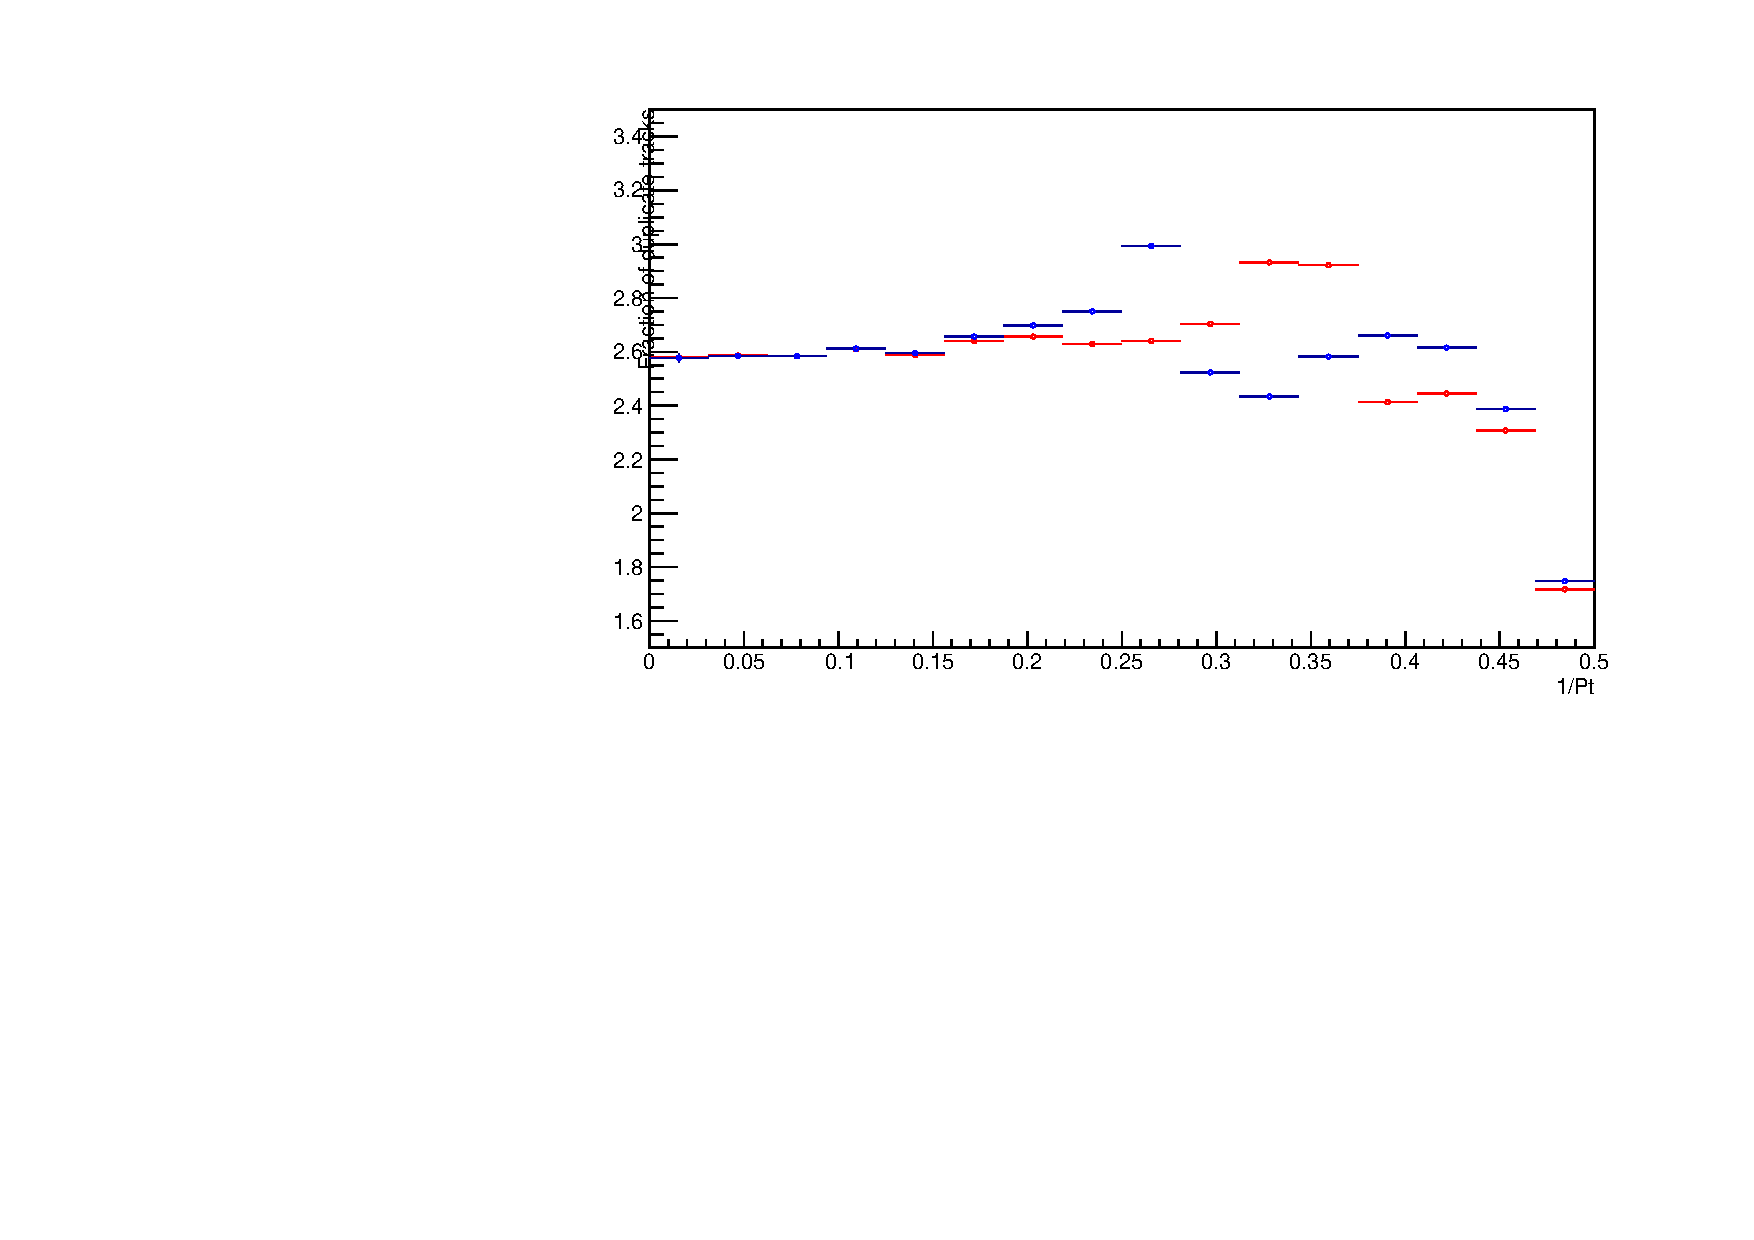
\includegraphics[width=0.47\textwidth]{figs/tk-upgrade/results-lowPtTracking/htFracDuplicatesVsInvPtTiltedGeometry_5000.pdf}
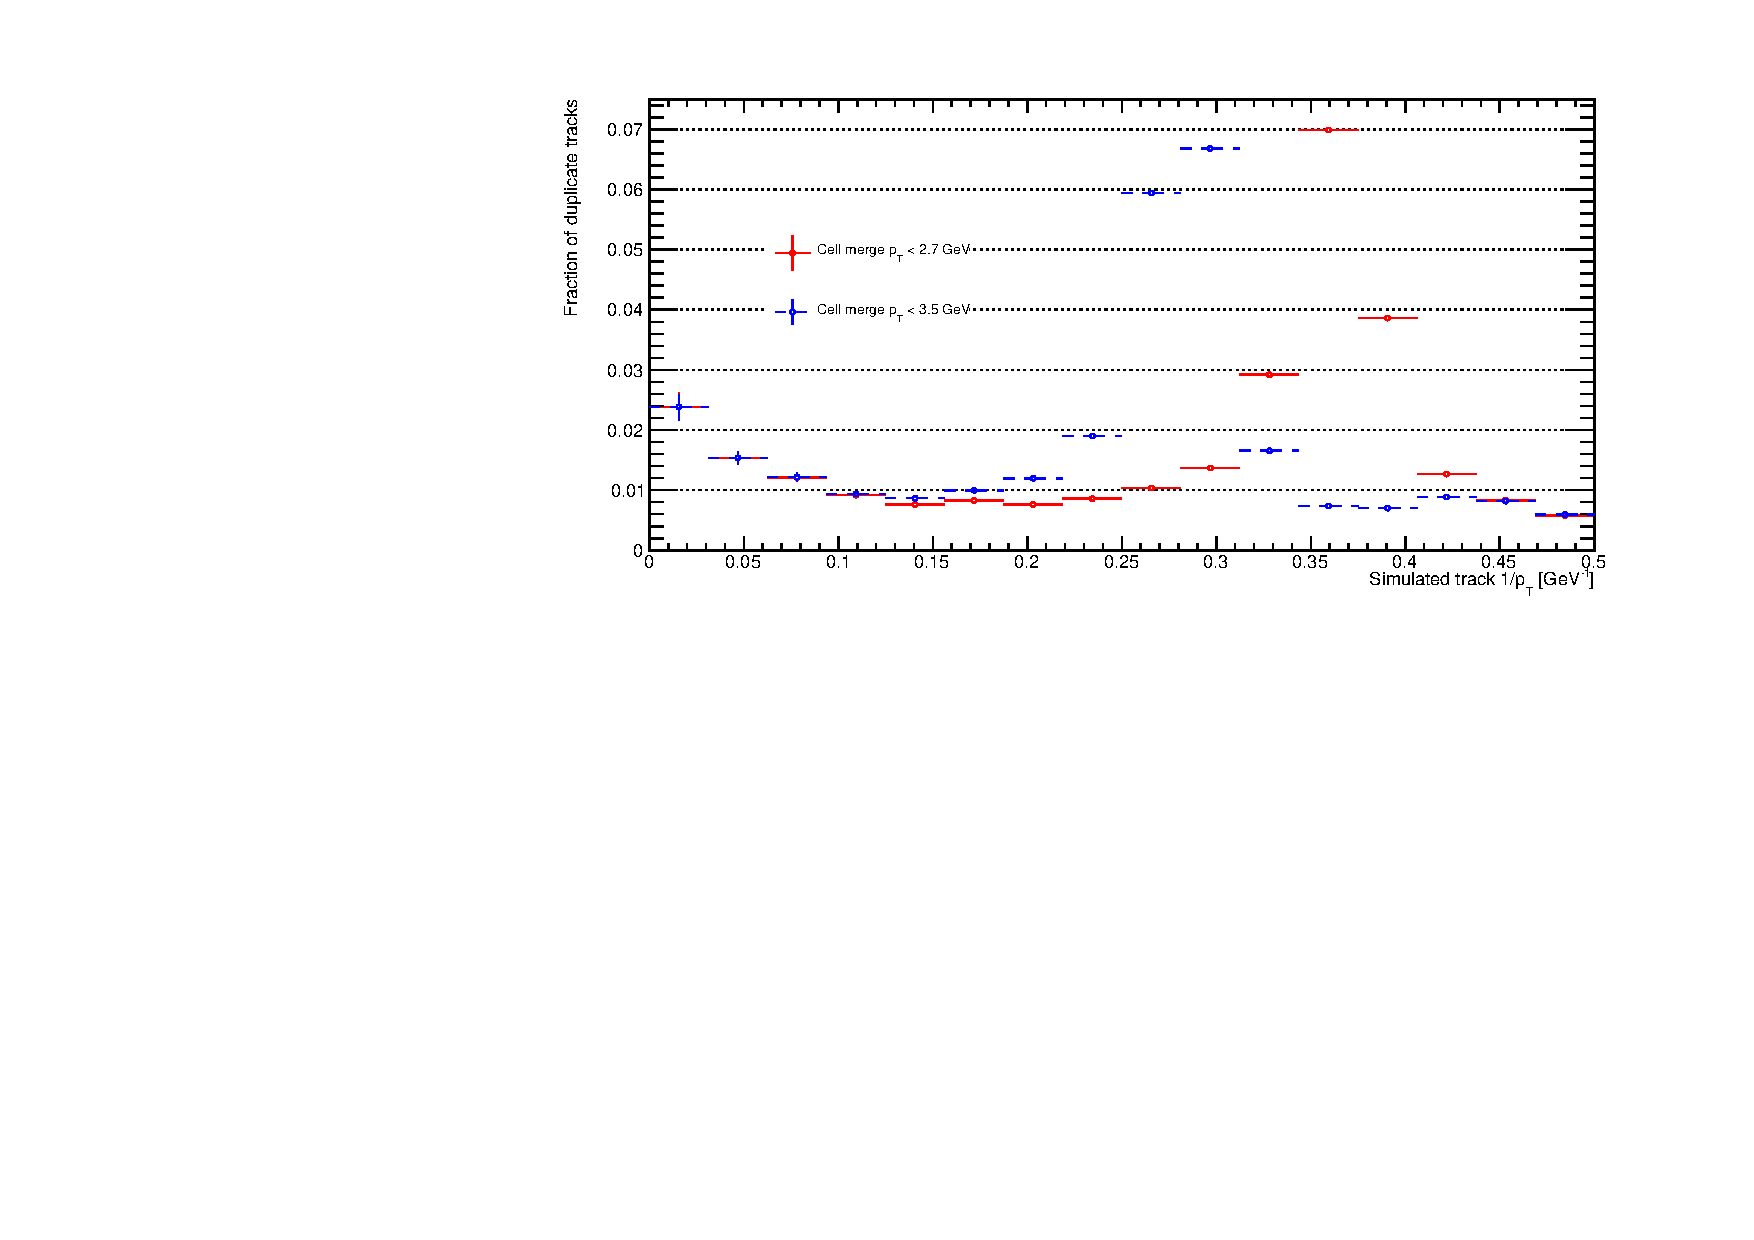
\includegraphics[width=0.47\textwidth]{figs/tk-upgrade/results-lowPtTracking/kfFracDuplicatesVsInvPtTiltedGeometry_5000.pdf}
\caption{The fraction of genuine tracks with duplicates as a function of $\frac{1}{\pT}$ following reconstruction by the \HT (left) and fitting and filtering by the \KF and \DR (right) for where the \HT cell merging \pT threshold is set to 2.7\GeV (red) and 3.5\GeV (blue). 
The constant coefficient for the \MS contribution was used for these \KF results.
\editComment{Resize plots!}
}
\label{fig:2GeVfracDups}
\end{figure}

\begin{figure}[tbp]
\centering
%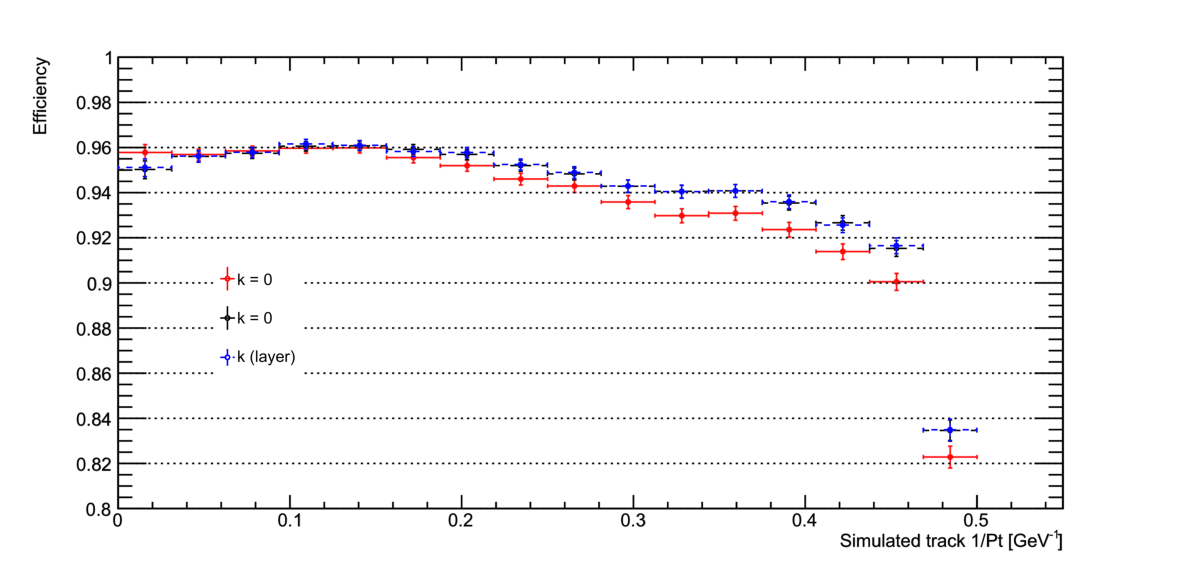
\includegraphics[width=\textwidth]{figs/tk-upgrade/results-lowPtTracking/kfTrackingEffVsInvPtTiltedGeometry_5000.pdf}
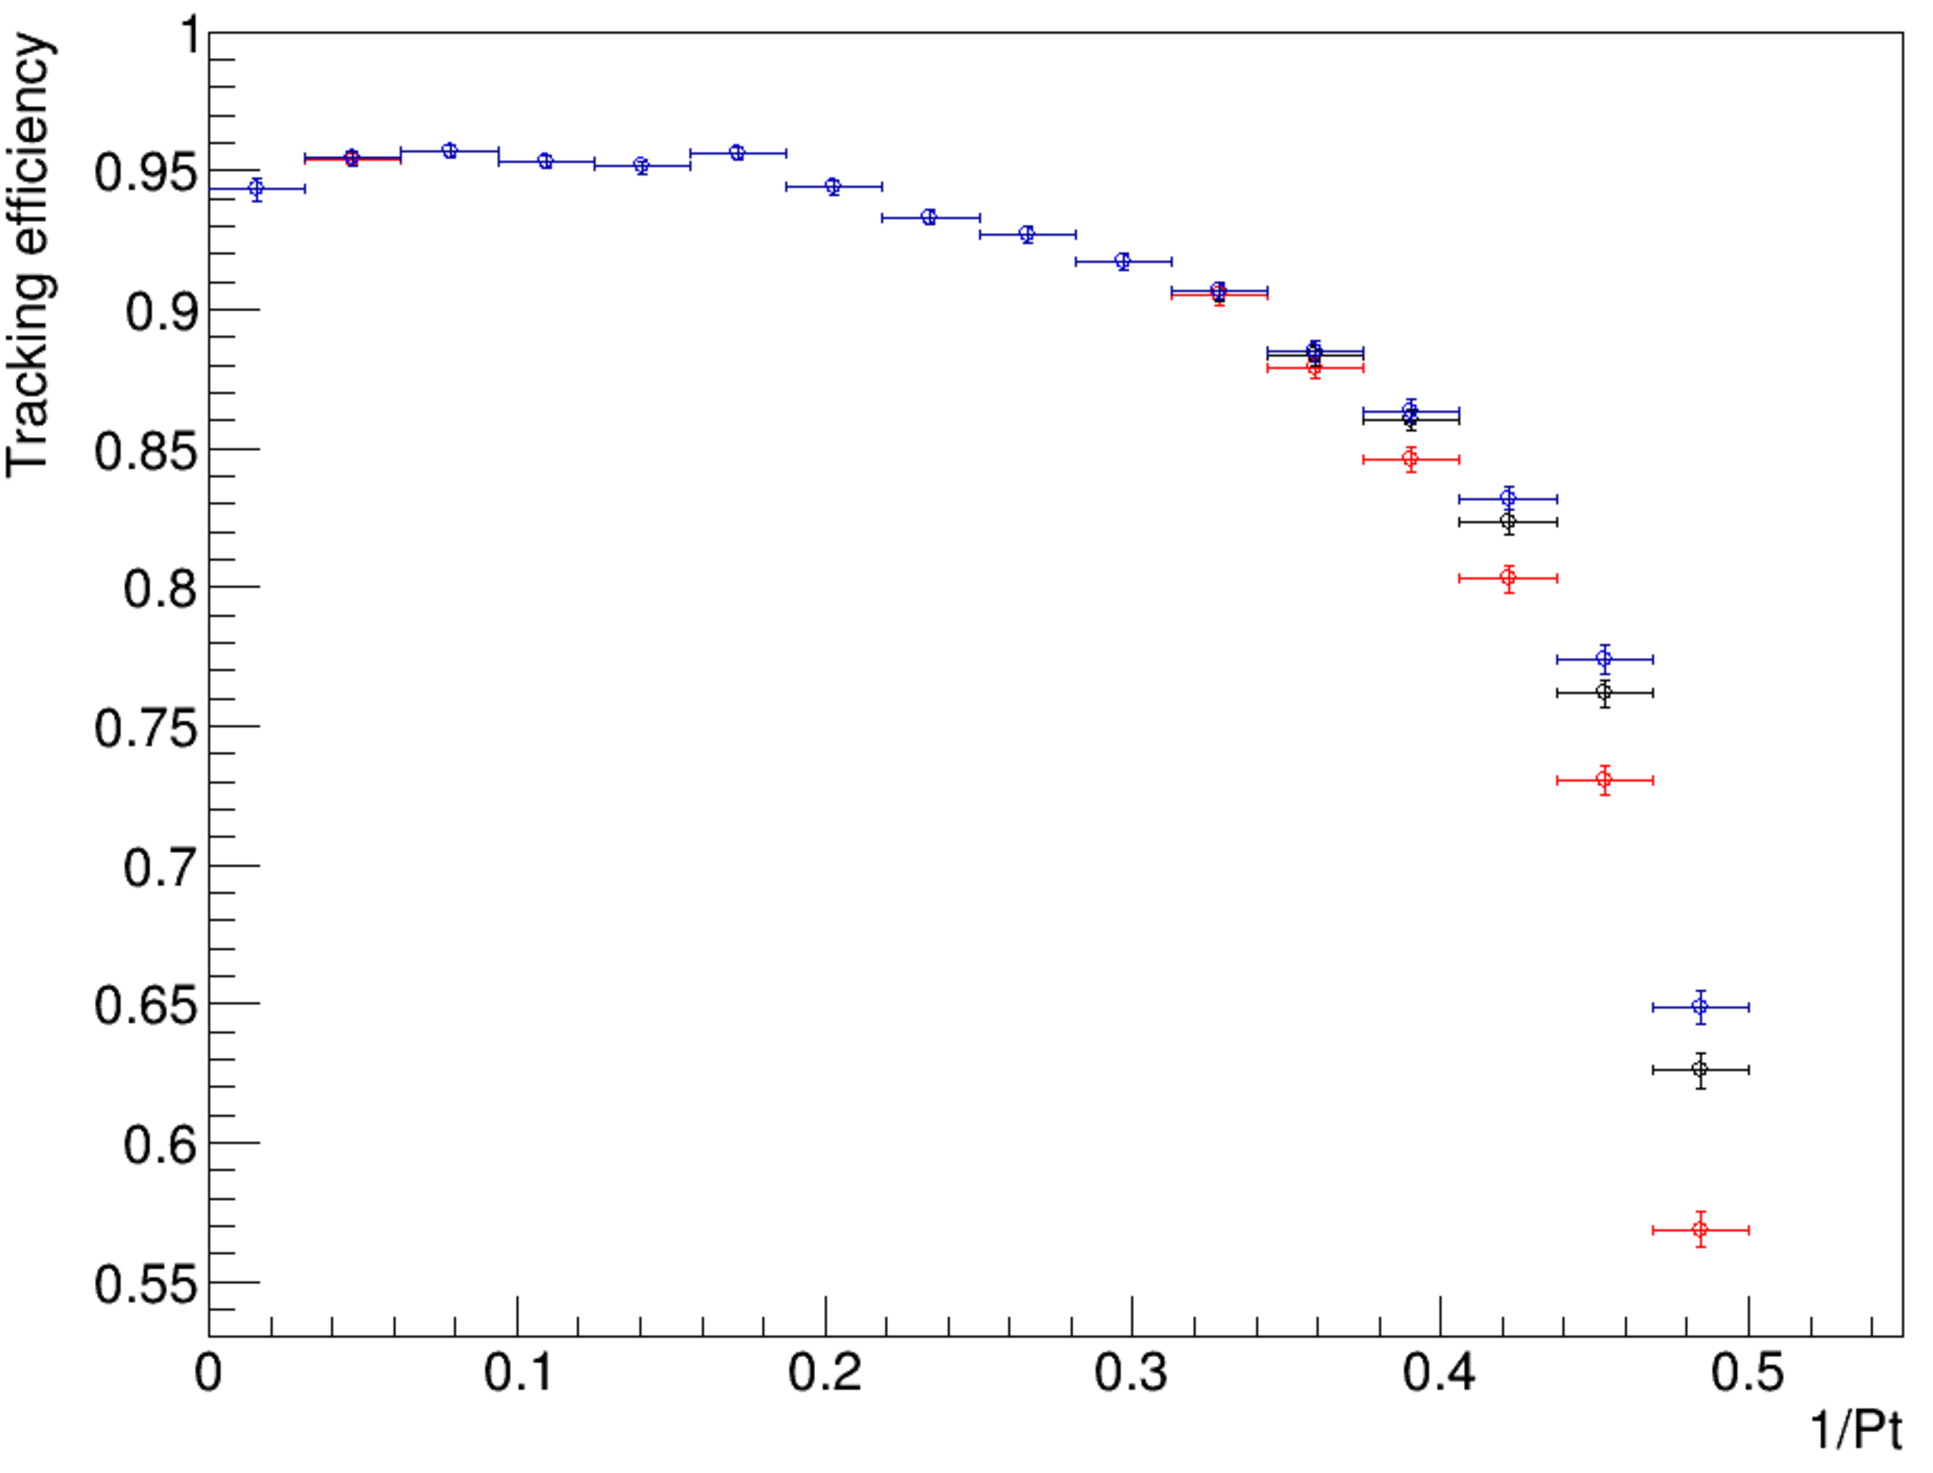
\includegraphics[width=\textwidth]{figs/tk-upgrade/results-lowPtTracking/kfTrackingEffVsInvPtFlatGeometry_5000.pdf}
\caption{Plots showing tracking efficiency as a function of $\frac{1}{\pT}$ for \ttbar events at \PU of 200 after the full chain has been run, where the \KF has not been modified to take \MS into account (red), a constant coefficient for \MS is used (black) and a layer dependent coefficient for \MS is used (blue).
\editComment{Figure needs updating.}
}
\label{fig:2GeVTiltEff}	
\end{figure}

Figure~\ref{fig:2GeVTiltEff} shows how the tracking efficiency for the whole chain improves when \MS is accounted for in the \KF.
The similar performance observed between the two coefficients in figure~\ref{fig:2GeVTiltEff} and table~\ref{tab:trackFindingPerformance2GeVKF} is due the amount of material traversed by a track not being constant for a single layer as the amount of material contributions in both the tracker and the prior contributions from the Inner Tracker, between the Inner and Outer Trackers and services varying as a function of $\eta$~\cite{P2TrackerTDR}.

Table~\ref{tab:trackFindingPerformance2GeVKF} also shows that compared to just the \HT optimisations alone, for both \MS  coefficients, the \KF is more capable at rejecting incorrectly reconstructed tracks by up to an additional 3-4\%.
In contrast, the duplicate increases for both coefficients by 3-5\% for the full chain, with the increase in duplicates occurring between $3.2\GeV$ and $5\GeV$, as shown in figure~\ref{fig:2GeVfracDups}, near the $3.5\GeV$ threshold for merging adjacent \HT cells.
At the time of writing this chapter, it is not understood how incorporating \MS into the \KF causes this, but it is suspected to be related to the use of the reduced precision of \HT cells.
\editComment{It is hoped that by the time of submission, someone (Ian ... ?) will have figured this out.}
%Tracks with \pt approaching the \pt threshold at which reduced precision of \HT cells are used are have the potential to be built out of both stubs from both the full and reduced precision \HT cells.

\begin{table}[htbp]
\topcaption {Track finding performance on simulated \ttbar events at a \PU of 200, after the \HT and the full chain (\HT + \KF + \DR) for the three differing \KF configurations where \MS is not considered (\emph{no \MS}), a constant \MS coefficient (\emph{$k$}) is used and a layer depedent \MS coefficient (\emph{$k(layer)$})is used. 
The track finding efficiencies following each stage are given using the efficiency definitions given in Chapter~\ref{subsubsec:helixParameter}, along with the mean number of tracks and the fraction of those tracks which are either fake or duplicate tracks.
\editComment{better to quote non-integer numbers and fractions of duplicates/fakes?}.
}
\label{tab:trackFindingPerformance2GeVKF}
  \centering
% This increases column spacing.
  \addtolength{\tabcolsep}{1ex}
% This right-aligns numbers in column, but centers them under column title.
  \begin{tabular}{ccr@{\hspace{4ex}}r@{\hspace{4ex}}r@{\hspace{4ex}}r@{\hspace{4ex}}r@{\hspace{4ex}}r@{\hspace{4ex}}r@{\hspace{4ex}}}
   \hline
   \bf{Configuration} & \bf{Stage} & \bf{Efficiency [\%]} & \multicolumn{1}{r}{\bf{Mean \# of tracks}} & \multicolumn{1}{r}{\bf{\% of fakes}} & \multicolumn{1}{r}{\bf{\% of duplicates}}  \\
   \hline
     & \bf{HT}     &  96.2 & 752.0 & 28.2 & 47.3 \\  
   No \MS  & \bf{Full Chain}     & 93.6 & 216.0 & 13.3 & 9.4 \\      
   \hline
   const $k$  & \bf{Full Chain}     & 94.2 & 216.3 & 10.3 & 11.2 \\      
   \hline
    $k(layer)$ & \bf{Full Chain}     & 94.2 & 222.1 & 10.8 & 12.3 \\  
   \hline
   
 \end{tabular}
 \addtolength{\tabcolsep}{-1ex}
\end{table}

Figure~\ref{fig:kfHelixParametersResVsInvPt} shows the resolutions of the track parameters as a function of transverse momenta in simulation for tracks originating from the primary interaction in \ttbar events at \PU of 200 for both \MS coefficients considered and for when \MS is not accounted for at all.
The resolutions of both \MS coefficients are superior across all \pt to when \MS is not considered at all, with the constant \MS coefficient typically providing more precise measurements than the layer dependent coefficient.  
As expected, lower transverse momenta tracks experience the greatest improvements given that \MS dominants at lower transverse momenta.
For both coefficients however, the \pt resolution resolution in the range $ 3.8 \GeV < \pt < 5.5\GeVc$ is worse than when \MS is not considered.
At the time of writing, this observation is still being investigated, but is suspected, like the increased duplicate rate in the same \pT range, to be related to the reduced precision of \HT cells.

\begin{figure}[htb]
\centering
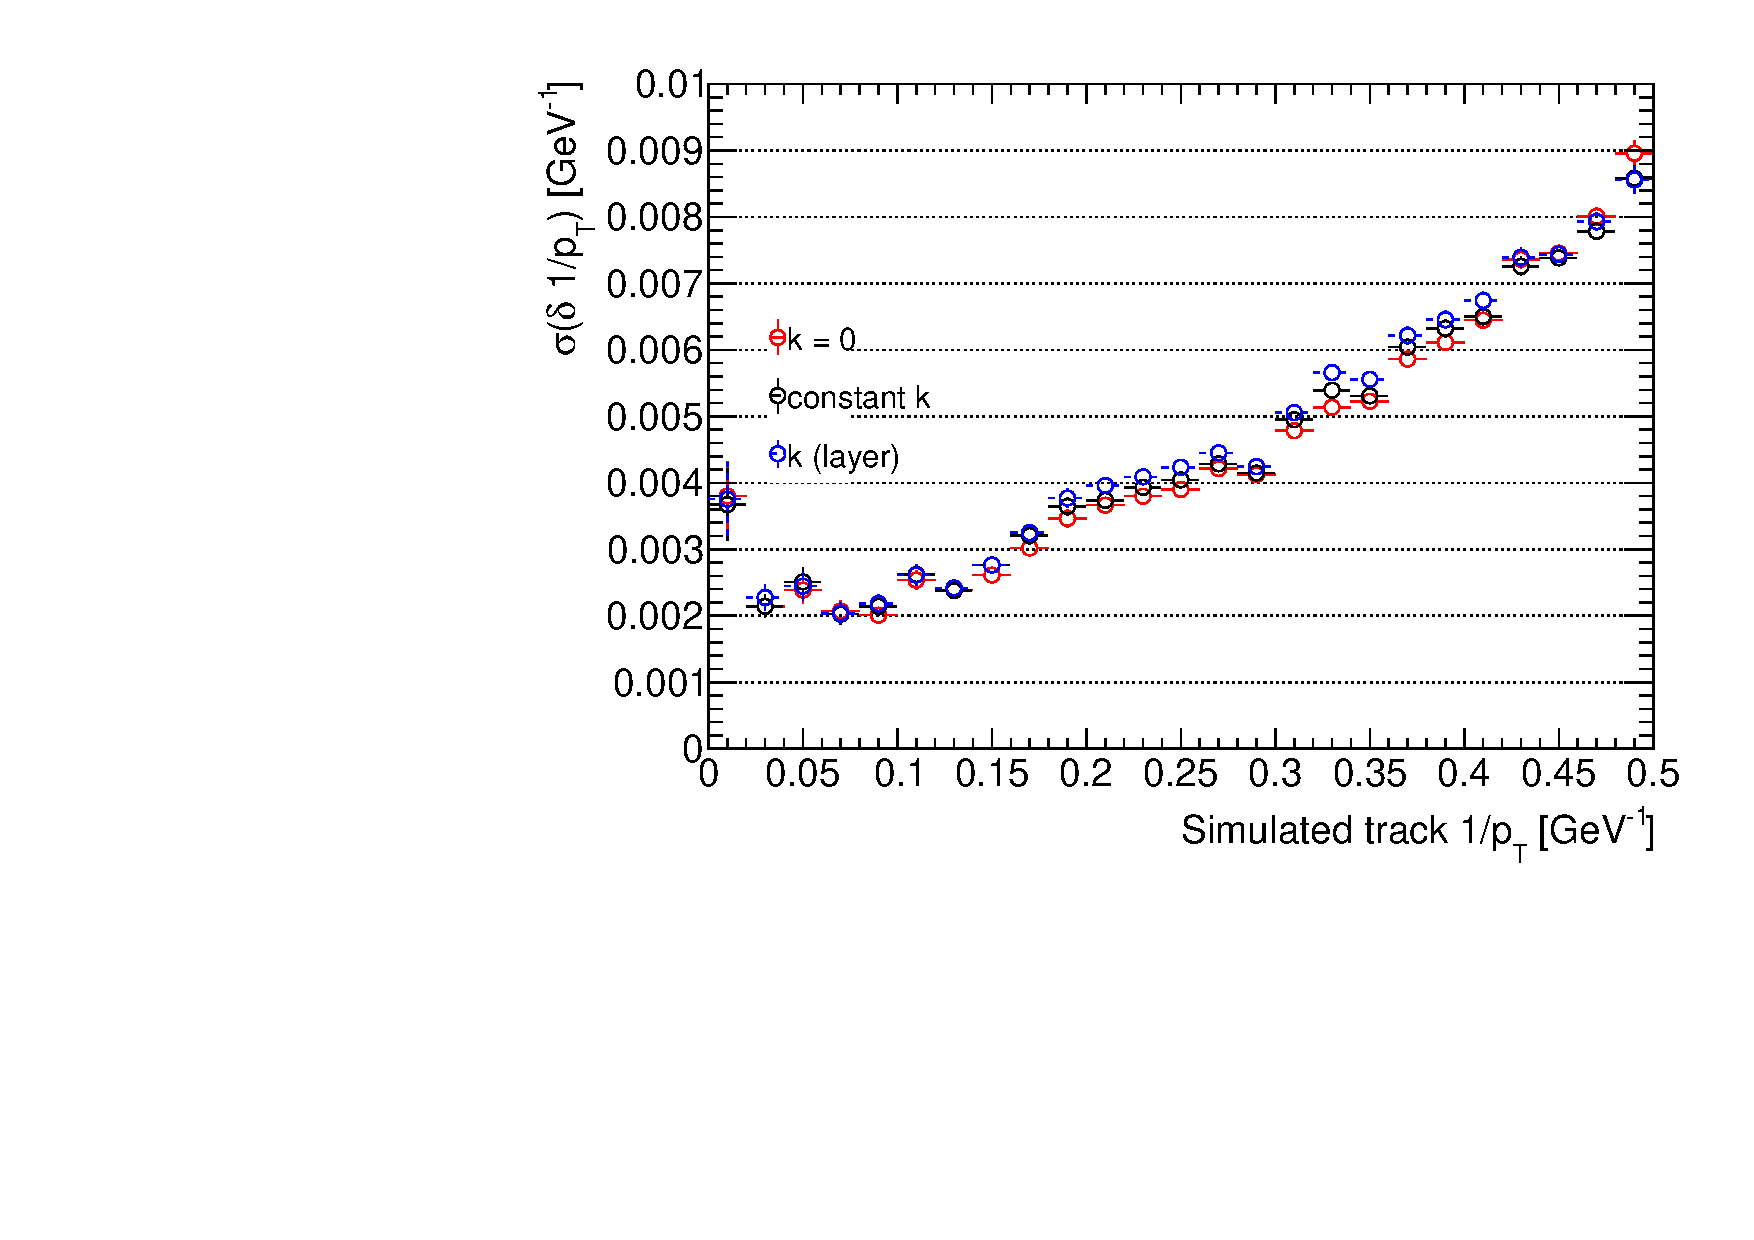
\includegraphics[width=0.47\textwidth]{figs/tk-upgrade/results-lowPtTracking/qOverPtResVsInvPtTiltedGeometry_5000.pdf}
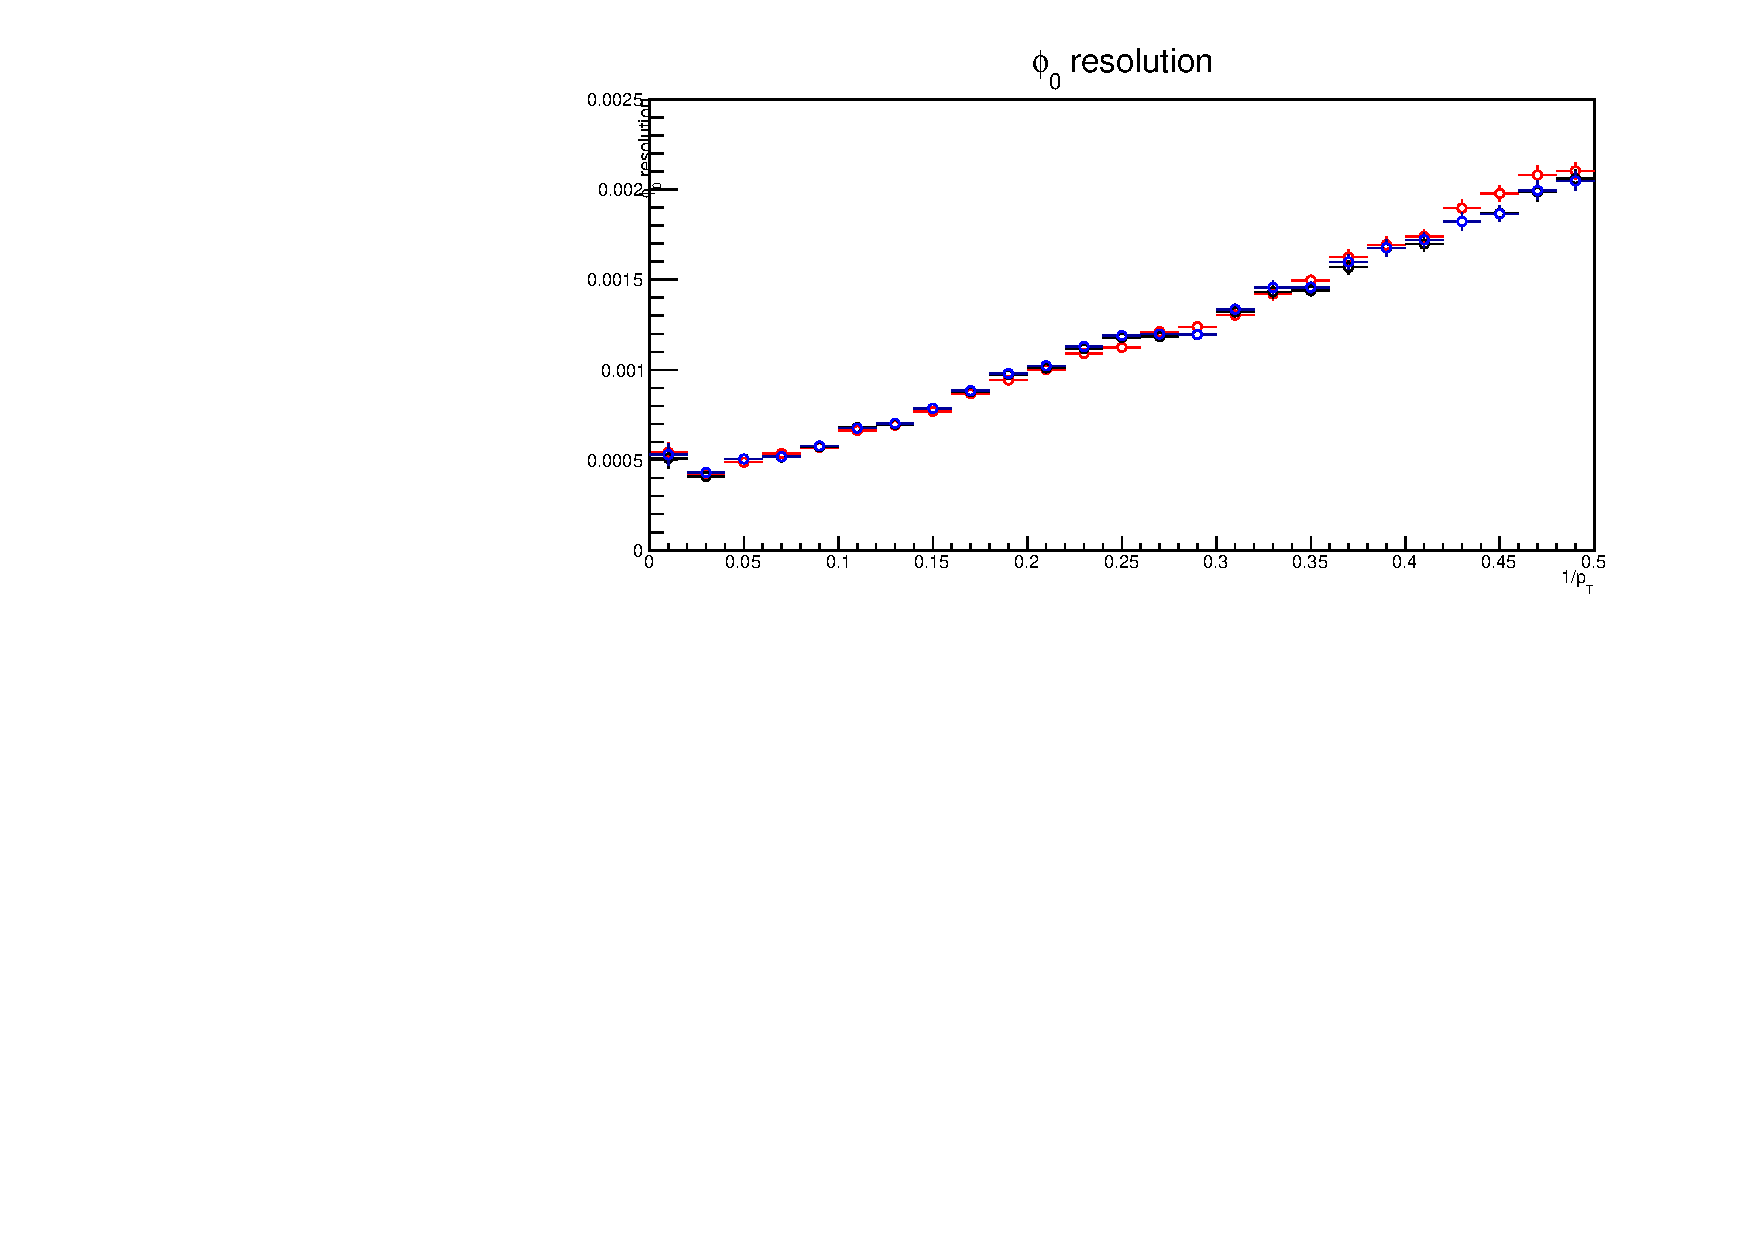
\includegraphics[width=0.47\textwidth]{figs/tk-upgrade/results-lowPtTracking/phi0ResVsInvPtTiltedGeometry_5000.pdf}
\\
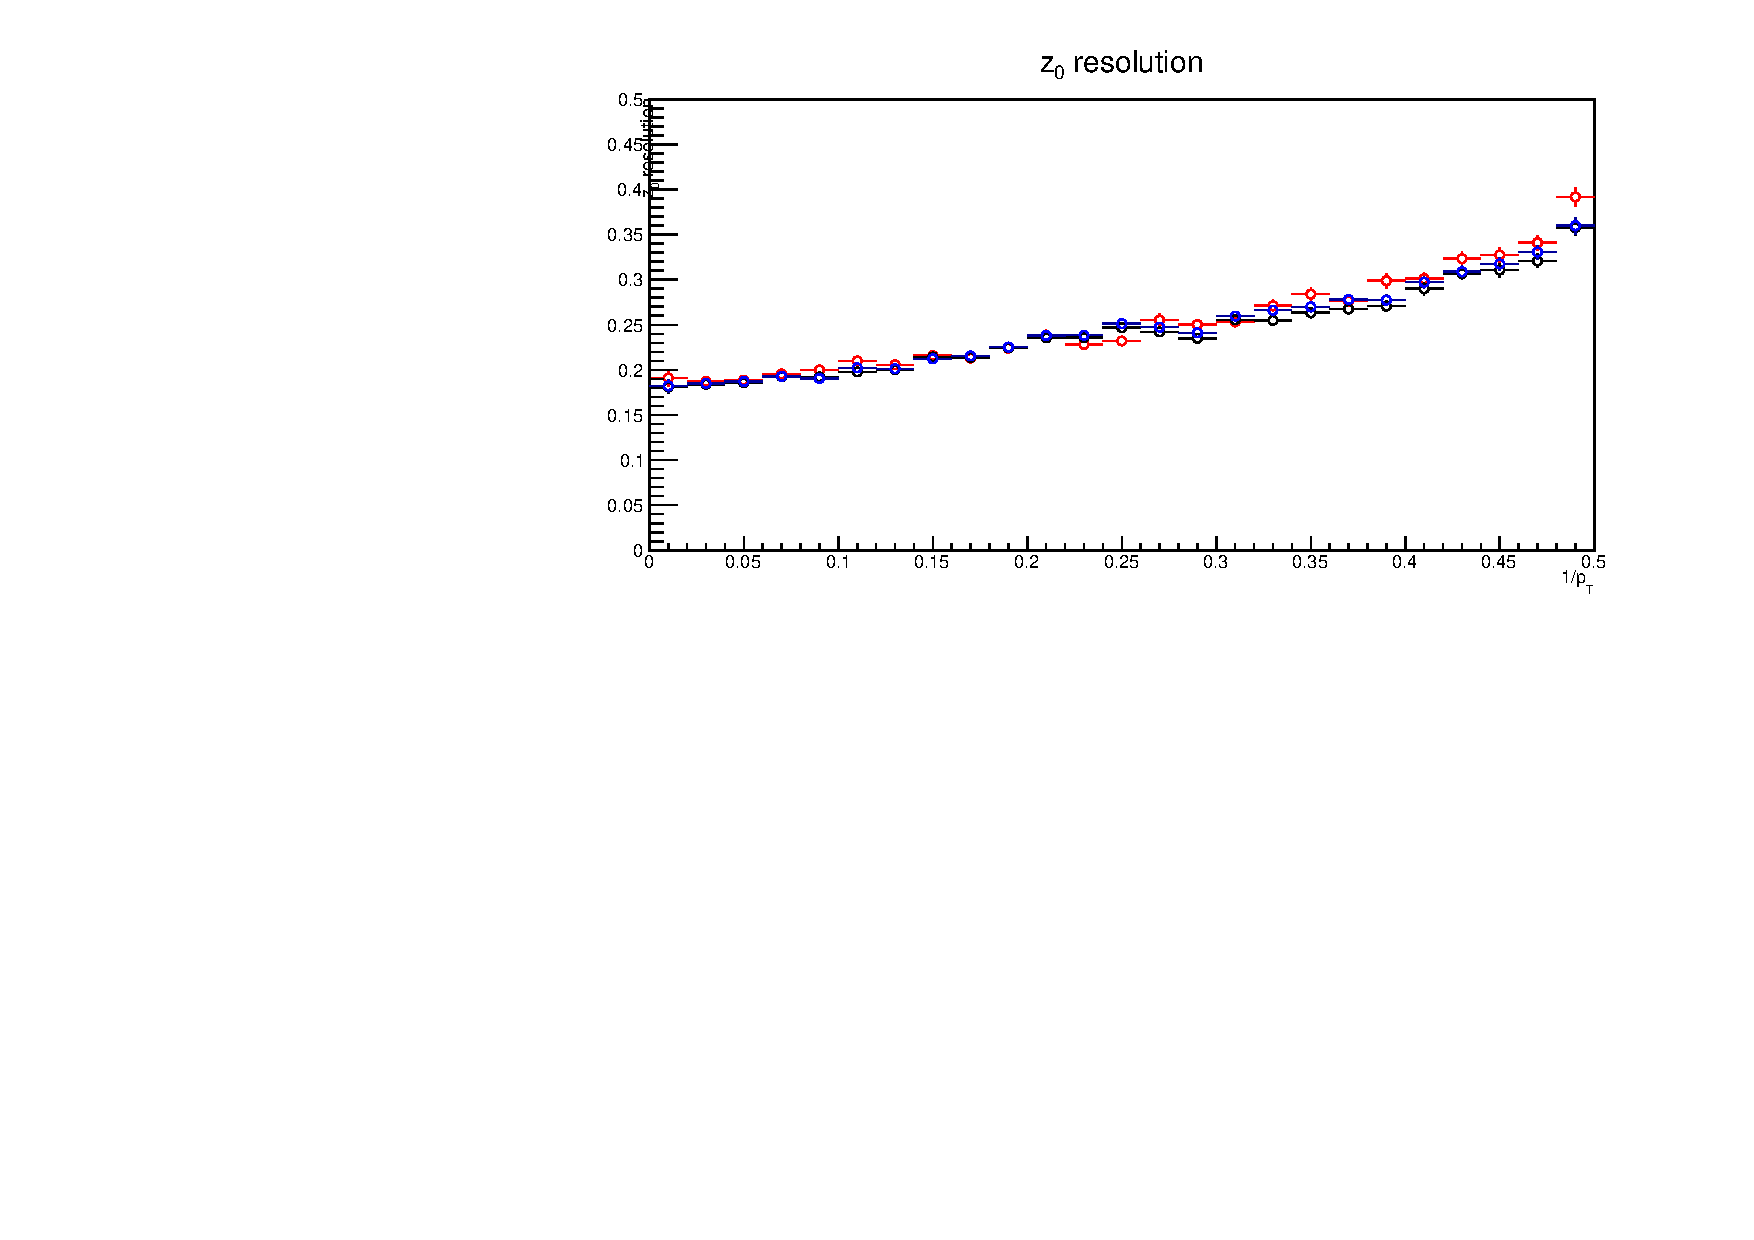
\includegraphics[width=0.47\textwidth]{figs/tk-upgrade/results-lowPtTracking/z0ResVsInvPtTiltedGeometry_5000.pdf}
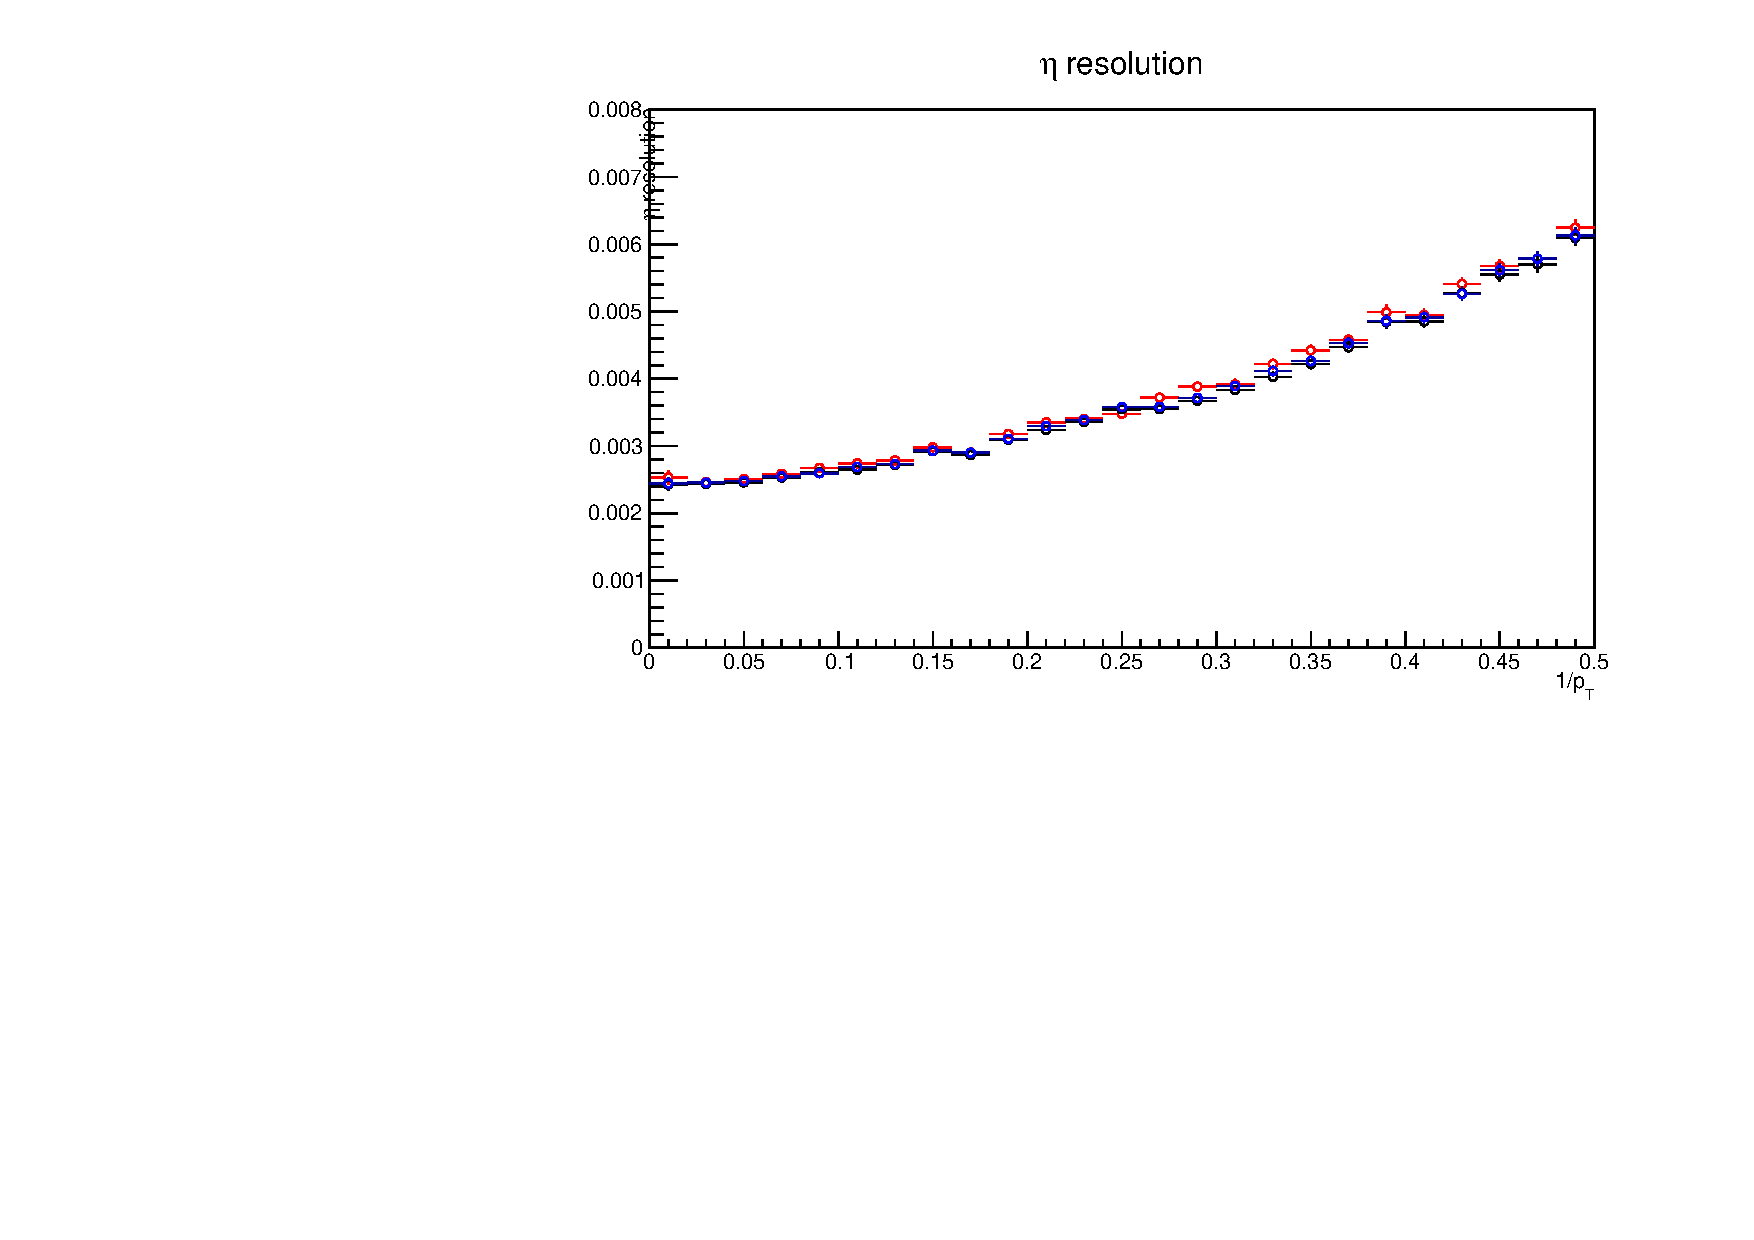
\includegraphics[width=0.47\textwidth]{figs/tk-upgrade/results-lowPtTracking/etaResVsInvPtTiltedGeometry_5000.pdf}
\caption{\pt resolution, $\phi$ resolution, $z_{0}$ resolution and $\eta$ resolution measured for primary reconstructed tracks in simulated \ttbar events at \PU of 200.}
\label{fig:kfHelixParametersResVsInvPt}
\end{figure}
